\chapter{Theoretical Background \& Fundamentals}
\label{chp:Background}
% \section{Relation to Chapter \ref{chp:Intro}}
In Chapter \ref{chp:Intro} the research regarding mitophagy is mentioned and the research to develop automated thresholding methods to streamline the data preparation process is detailed in terms of objectives and the proposed use case. Before detailing related research or the design of the proposed thresholding system an initial establishment of theoretical information regarding the mitophagy research use case will be presented. This theoretical information will regard the organelles being imaged for mitophagy analysis, the mitophagy process itself, the microscopy techniques employed for imaging, an overview of image preprocessing techniques that may be employed (noise removal, deconvolution, thresholding) and other particular techniques of interest to the thresholding system design.

\section{Mitophagy and involved organelles}\label{sec:mito_detail}
%In Section \ref{sec:background} the motivations for researching the Mitophagy process are raised including the stipulation of the organelles of interest for this Mitophagy research. To briefly reiterate these points, mitophagy as a process involves the recycling of overly damaged mitochondria to maintain mitochondrial health in cells where dysfunctional mitophagy has been observed in a number of illnesses. For the purpose of this proposed Mitophagy research, the cellular organelles involved with the mitophagy process that is being imagined will be discussed further in function and structure.
In Section \ref{sec:background} a number of potential applications of mitophagy research were presented. Of importance were the overview of the organelles involved in mitophagy, the purpose of these organelles and the importance of mitophagy with regard to these organelles. As these organelles and the mitophagy process will studied via visual and image analysis the function but also the structure will be discussed further in this section.
\subsection{Mitochondria}\label{sec:mitochondria}
Mitochondria are organelles found in plants, animals and many other multicellular organisms that are primarily responsible for supplying the energy required by the cell. The primary functions and mitochondria structure will be discussed in this section.
\subsubsection*{Functions}
The mitochondria perform a number of functions within the cell but the most notable function is the provision of fuel for the cell for the other contained organelles to play their role in maintaining the cell and executing their actions relative to the rest of the cells. This fuel is synthesized by the mitochondria in a molecule called adenosine triphosphate (ATP) which is an efficient fuel format accepted by all other energy-consuming organelles within the cell. This is crucial to the survival of cells as the many chemical and mechanical actions performed by cells can be energy expensive and the extraction of energy from food energy molecules is of a low yield with much of the desired energy remaining chemically trapped~\cite[p. 33, 35, 40]{cell_phys_book}. For this reason, mitochondria are dedicated to producing ATP which effectively yields energy when required and the number of mitochondria in cells ranges from hundreds to thousands depending on the cell functions. This is not the sole function of mitochondria as they are instrumental in the management of controlled cell death (apoptosis) which is employed when the cell itself is too damaged for repair deeming it to be of risk to the surrounding cells~\cite[p. 40-41]{cell_phys_book}.
\subsubsection*{Structure}
The structure of mitochondria is that of an oval-like structure with many cristae (internal folds) increasing the internal surface area and improving the efficiency of ATP synthesis process. A visualisation of this internal structure can be seen in Figure \ref{subfig:mito_folds} and these mitochondria coexist separately from each other in the cell in a formation called `punctate' or they can appear in a formation called a `reticulum'. A mitochondrial reticulum (shown in Figure \ref{subfig:mito_retic} is formed primarily in cells with a higher energy demand than usual such as skeletal muscle and this reticulum is akin to a connected branching structure. This branching allows mitochondria to support each other by sharing functional components as ATP production can cause wear to build up as a byproduct.
\begin{figure}
    \centering
    \subcaptionbox{Image of an individual mitochondria\label{subfig:mito_folds}}{\stackinset{r}{}{t}{}{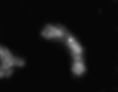
\includegraphics[width=0.1\linewidth, cframe=orange 1pt]{figs/ch2figs/Crop_punctate.png}}{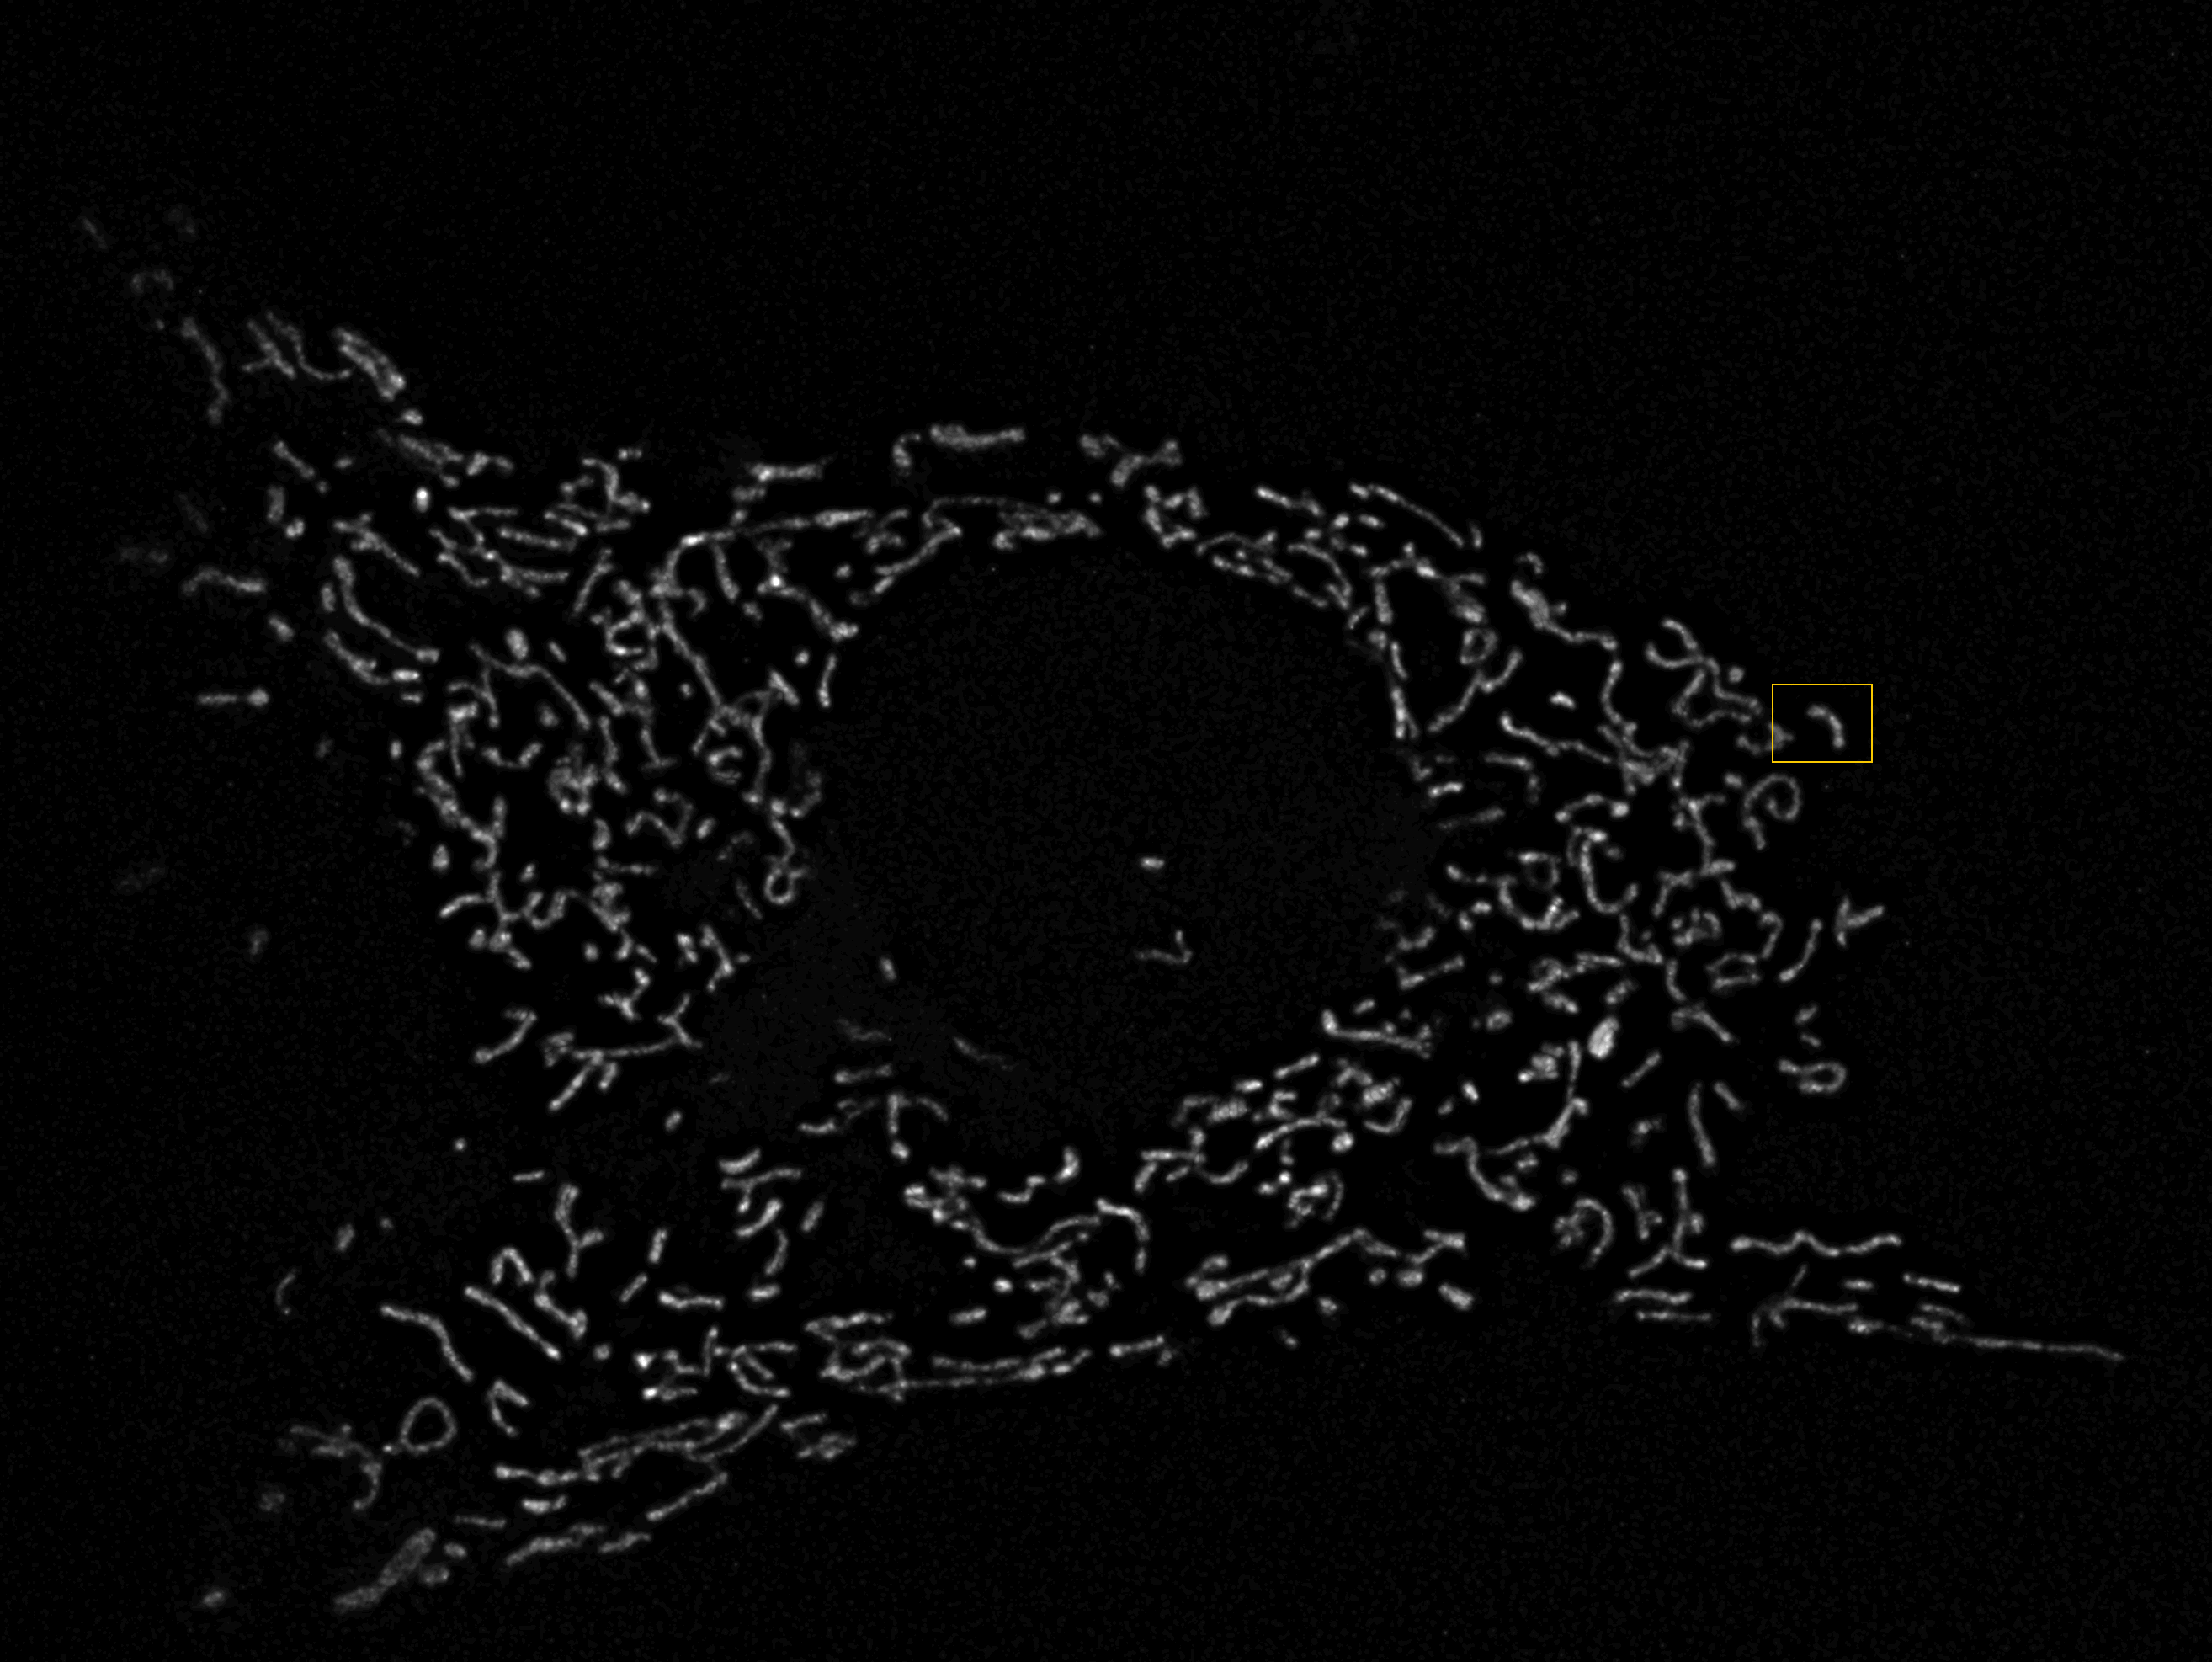
\includegraphics[width=0.49\linewidth]{figs/ch2figs/MAX_CCCP_1C=1T=0_punctate.png}}}
    \subcaptionbox{Image of the mitochondrial reticulum\label{subfig:mito_retic}}{\stackinset{r}{}{t}{}{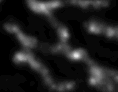
\includegraphics[width=0.1\linewidth, cframe=orange 1pt]{figs/ch2figs/Crop_branched.png}}{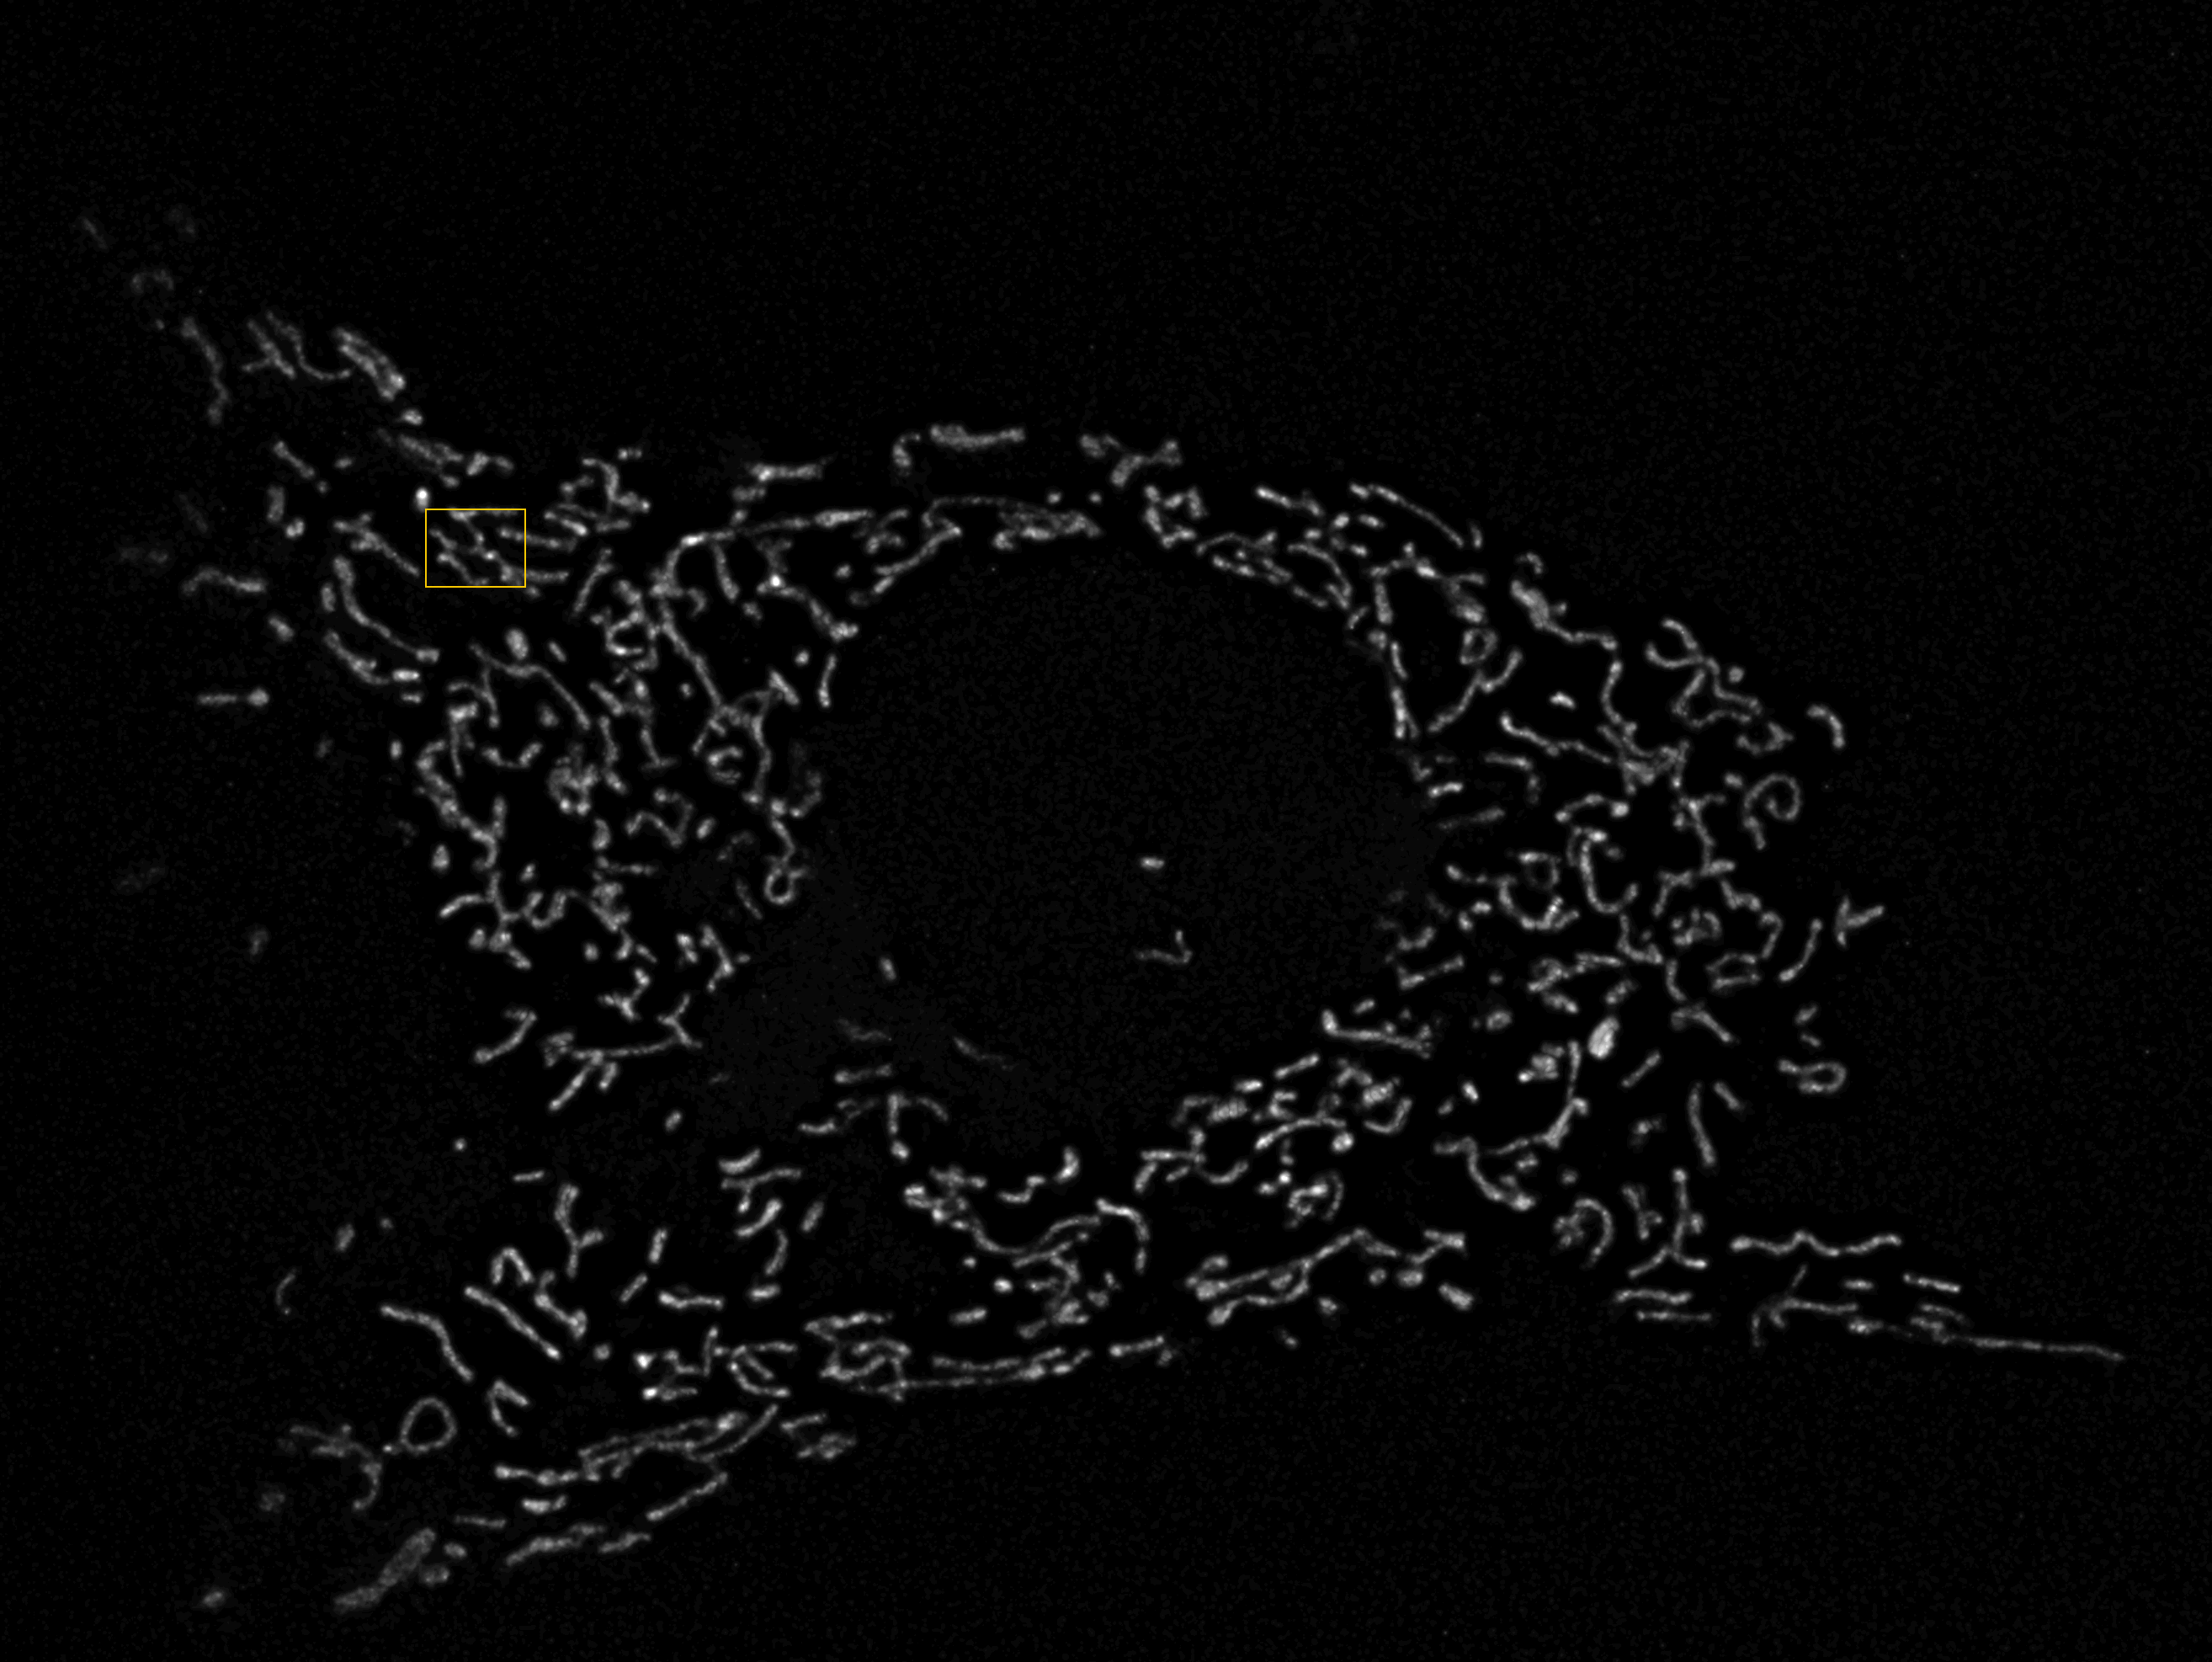
\includegraphics[width=0.49\linewidth]{figs/ch2figs/MAX_CCCP_1C=1T=0_branched.png}}}
    \caption[Comparison between punctate and branching mitochondria structures]{Comparison between mitochondria structure types with (\subref{subfig:mito_folds}) singular punctate mitochondria and (\subref{subfig:mito_retic}) branching mitochondria forming a reticulum}
    \label{fig:mito_struct}
\end{figure}
\subsection{Lysosomes}\label{subsec:lysosome}
Lysosomes are organelles involved with the recycling and degradation of compounds and organelles within the cell.
\subsubsection*{Function}
The purpose of lysosomes is to decompose compounds within the cell into the base components which can be used to synthesize new organelles or provide needed nutrients. The lysosome is a carrier of hydrolases (an enzyme that reacts with water to break down molecules) that break down specific compounds within the cell ranging from biomolecules absorbed from outside the cell such as proteins, carbohydrates and lipids; to invasive bacteria; and even damaged organelles. The breaking down of compounds absorbed from outside of the cell (through a process called endocytosis) is used to `digest' these compounds to provide a source of new nutrients. The decomposition of invasive bacteria and damaged organelles acts similarly to a defence response to maintain the health of the cell while also allowing the damaged organelles to be recycled to produce new organelles maintaining the population of healthy organelles~\cite{lyso_auto_relation, cell_phys_book}. The process of decomposing these compounds is called \textit{autophagy} and relies on autophagosomes to deliver the compounds, to be decomposed, to the lysosomes. The lysosome fuses with the autophagosome to become an \textit{autolysosome} where the contained compounds are introduced to hydrolase enzymes initiating decomposition~\cite{lyso_auto_relation}.
\subsubsection*{Structure}
Lysosomes are small structures of spherical bodies composed of a membrane-like structure containing the hydrolase enzymes~\cite{cell_phys_book}. This membrane structure is impermeable to most interfacing to prevent the unintentional release of the contained enzymes~\cite{lyso_auto_relation}.

\subsection{Autophagosomes}\label{subsec:autophagosome}
Autophagosomes are the name for the membrane structure that carries compounds to be decomposed by autophagy.
\subsubsection*{Function}
Autophagosomes are formed from phagophores (a cup-shaped membrane) that are located in the cytosol (cellular fluid) and stretch to engulf the compounds to be decomposed. Once the compounds have been engulfed the phagophore is referred to as an autophagosome which proceeds to carry the contents to a lysosome. An autophagosome is one of the organelles capable of interfacing with lysosomes to form an autolysosome. After fusing together the lysosome introduces the enzymes to the cargo of the autolysosome and autophagy begins~\cite{lyso_auto_relation}.
\subsubsection*{Structure}
An autophagosome is initially a single membrane called a phagophore which stretches and deforms into a cup-like shape when approaching biomolecules that are supposed to undergo autophagy. The phagophore continues to stretch around the biomolecules until they are fully engulfed at which point the edges of the cup-like shape join and fuse to form a double membrane. The phagophore is now referred to as an autophagosome with a complete double membrane which has an ovular/spherical shape.

\subsection{Mitophagy}
With the relevant organelles, and their functions, briefly covered a simple description of the mitophagy process can be presented. As mentioned in Section \ref{sec:background}, the dysfunction of mitophagy is associated with a number of diseases with neurodegenerative disorders (e.g. Parkinson's disease, Alzheimer's disease, etc.) of note. Mitophagy as a process refers to the isolation and subsequent decomposition of dysfunctional mitochondria. This is performed by the autophagosomes engulfing the mitochondria and transporting them to lysosomes as cargo. The autophagosomes fuse with the lysosomes introducing enzymes to the mitochondria and beginning the decomposition process. After the decomposition is completed the resultant molecular components of the mitochondria can be used by the cell in a number of ways such as synthesising new mitochondria.\par The reasons why mitochondria are degraded by autophagy is typically due to irreparable mitochondria dysfunction usually caused by either physical, chemical or oxidative damage. This damage to the mitochondria can affect a number of components (mitochondrial DNA, lipids, proteins, etc.) that are necessary for many mitochondrial functions and while this damage is below a certain threshold the impact of this damage on mitochondrial functions can be mitigated through fusion. This fusion entails the joining of mitochondria to share functional components to compensate for those that are damaged allowing mitochondrial functions, like ATP synthesis, to continue~\cite{MitoFus-2012}. Multiple fusions can occur between mitochondria allowing branching chains of mitochondria to form, mentioned in Section \ref{sec:mitochondria} as a mitochondrial reticulum, which is more frequently seen in cells undergoing high ATP demand such as activated skeletal muscle cells~\cite{cell_phys_book}. This makes the network of fused mitochondria robust to interference in ATP production when there are high energy demands.\par 
Previously it was mentioned that fusion could compensate for damage to the mitochondria given that the damage is below a threshold but what happens when this threshold is exceeded? When this occurs the mitochondria can be seen as irreparable and if present in a reticulum then the density of dysfunctional components could place undue strain on the fused mitochondrial collective. The first step in this process is mitochondrial fission where dysfunctional components are aggregated to a singular region within the mitochondria which are then split into two daughter mitochondria. The daughter mitochondria containing dysfunctional components can then be removed via autophagy while the healthy daughter can resume activities. In the case of a fused mitochondria network, this aggregation still occurs and only the localised region containing the dysfunctional components will be split from the network~\cite{MitoFus-2012}.\par With the dysfunctional mitochondria separated from the healthy a number of mitochondria-specific biochemical pathways (mechanisms), which will not be described further here, activate flagging the dysfunctional mitochondria. With the dysfunctional mitochondria flagged and located the phagophores can engulf the mitochondria, becoming an autophagosome, and transport it to a lysosome to begin decomposition~\cite{MitoMechan, MitoFus-2012} (described in Sections \ref{subsec:lysosome} and \ref{subsec:autophagosome}).

\section{Fluorescence Microscopy} \label{sec:fluorMicr}
%For cluster tracking and detection for cells: https://link.springer.com/article/10.1007/s40846-016-0216-y
As described in Section \ref{sec:background}, a particular method of studying mitophagy behaviours is to study the organelles involved in this process (detailed prior in Section \ref{sec:mito_detail}). There are a number of methods by which to analyse organelle behaviours whether visual or biochemical where each captures different ranges of traits describing these behaviours. For the study of mitophagy, it is not uncommon to employ a combination of visual and biochemical analysis but it is the visual analysis that is of interest to this particular research. This section will explore the high-level motivation behind fluorescence microscopy as opposed to traditional optical microscopy, the factors to consider for suitable fluorophore selection, the limitations of fluorescence microscopy, an overview of confocal fluorescence microscopy, and a brief breakdown of the relevant microscopy apparatus.

\subsection{Light microscopy and motivations for fluorescence microscopy}\label{sec:lightVsFluoro}
In the microscopy of both cellular and subcellular structures, there are numerous biochemical structures, biomolecules and intracellular processes that can be observed. For this research, organelles are the subcellular structures that are of interest and going forwards will be referred to simply as `structures'. A traditional, and still used, method to visually observe these structures is through the use of optical microscopy. 
\paragraph{Optical microscopy} exposes the biological specimen, placed on the microscope stage, to visible spectrum light illuminating the specimen allowing cells, organelles, and other biochemical structures to be seen. When imaging these specimens there are three obstacles to making accurate and clear observations of the specimen, particularly with subcellular objects. These are the resolution limit where optical microscopes struggle to resolve features (edges, gaps between structures, etc.) that are smaller than $0.2\mu$m~\cite[p.582]{GeneralMicroscop}; thick specimens reduce the level of clear detail at higher resolutions; and that these specimens are frequently composed of majority water thus structures and features may be indistinct if not nearly invisible~\cite[p.585]{GeneralMicroscop}. The challenge of thick specimens can be resolved by slicing the specimen and improving the clarity due to the high water contents can be resolved through the use of stains which bind to cell structures, bacteria and other microscopic organisms based on the stain's preferred conditions. This allows stains to be selected that will localise to specific structures or to specific cellular processes (e.g. metabolic) improving the contrast between these structures from the irrelevant surroundings. Despite this, there can still be visual interference from surrounding structures which can decrease the clarity at which fine structures or features can be discerned.\par 
\textcolor{red}{For the above paragraph, and in future, I use the paragraph{} command to head off new points in the subsubsection that is contained within the paragraph. I realise now, after going through a few sections, that there are extra spaces after the bolded paragraph heading. Do you think this looks fine, should I linebreak after the paragraph heading, or do you think I should bold text the first word (as I have done now) but without the space after which will use textbf and linebreak to replicate the effect.}
\paragraph{Fluorescence microscopy} is similar to optical microscopy except for the types of stains utilised and some adjustments to the microscope architectures. Fluorescence microscopy utilises fluorescent stains, called fluorophores, that are identical to the stains described prior except that they emit light of a specific wavelength (based on the fluorophore) when excited. This excitation of the fluorophores is likewise induced by exposing these fluorophores to the light of a fluorophore-specific wavelength allowing the selection of which structures are visible by constraining both the wavelength of light illuminating the specimen and the wavelength that is captured by the microscope. This wavelength selection for both the excitation and emission light is achieved through filters that reject wavelengths outside of the currently selected range allowing structures to be indicated by specific wavelengths~\cite{Sanderson-2014}. For this reason, fluorescent stains can be referred to as indicators and fluorescently stained structures can be referred to as `indicated' where post-imaging different colours can be assigned to these respective wavelengths improving differentiation between different types of indicated structures. A comparison between optical and fluorescence microscopy can be seen in Figure \ref{fig:microscopeTypeCompare}.

\begin{figure}[h]
    \centering
    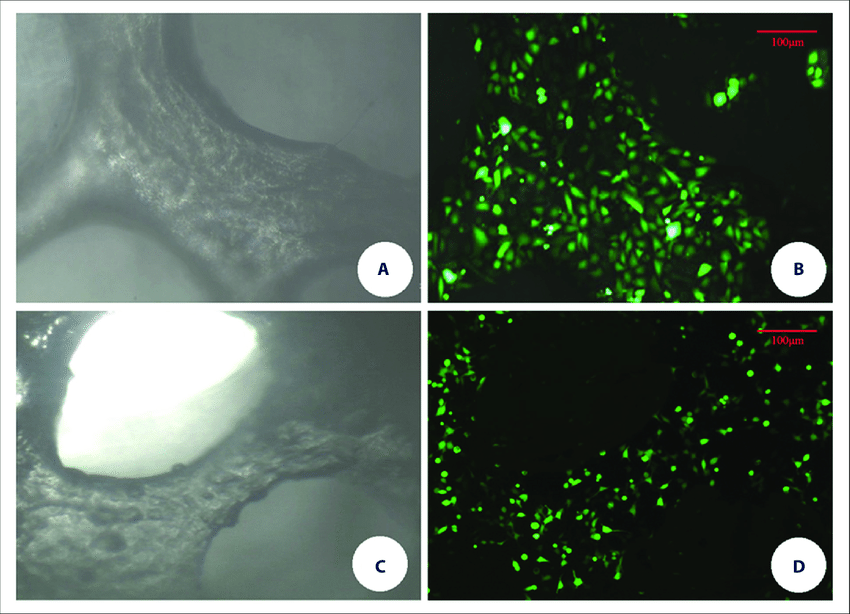
\includegraphics[width=0.6\textwidth]{figs/Light-microscope-and-fluorescence-microscope-observation-of-DBM-scaffolds-under-dynamic.png}
    \caption[Visual comparison between light and fluorescence microscopy]{A comparison between light (left sub-figures) and fluorescence (right sub-figures) microscopy. The same specimen is represented using each microscopy type with the top pair (A,B) and the bottom pair (B,D) each representing different cell cultures\cite{microscopeTypeFig}.}
    \label{fig:microscopeTypeCompare}
\end{figure}

\subsection{Factors regarding fluorophore selection for fluorescence microscopy}\label{sec:FluoroProcess} 
As described in Section \ref{sec:lightVsFluoro}, the primary reason to use fluorescence microscopy is the ability to select structures or biomolecules that are relevant to the analysis through the use of specific fluorophores. When imaged the indicated objects appear with greater clarity and differentiation than in optical microscopy through the rejection of irrelevant fluorescence. These benefits are not acquired without a cost which is the added decision-making of selecting suitable fluorophores for the analysis being performed. There are a number of factors involved in this can be viewed as the types of biomolecules being stained (for our mitophagy imaging purposes it is the organelles) and the fluorophore properties.\par Regarding the impact on fluorophore selection the largest is based on what biomolecules or structures are of interest to the analysis as the scope of fluorophores will be narrowed to those that suitably stain them after which the fluorophore properties are to be considered in the context of the imaging requirements. Imaging requirements can describe the status of the specimen whether alive or fixed; the duration of the imaging whether time-lapse is being performed; the desired signal strength of the captured fluorescence; and the number of fluorophore types employed such that the different types of structures of interest can be differentiated between.\par The fluorophore properties that will be explored are the excitation spectrum, the emission spectrum, the photostability, the maturation time, and the emission brightness~\cite{fluorophorePick, fluoro_properties_2, fluorophore_article}.

\paragraph{Excitation spectrum} is the range of wavelengths that are able to excite the indicators to induce emission. The excitation spectrum of a fluorophore must be evaluated relative to the microscope filters for the illuminant and the excitation spectra of indicators for other structure types. When the excitation spectra of two or more different fluorophores overlap, a phenomenon called `cross-talk' is induced~\cite{Bolte-2006}. This overlap can be complete or partial where the quantity of overlap can increase the severity of the cross-talk where cross-talk causes the simultaneous excitation of multiple fluorophores where only one fluorophore type was intended to be excited.
\paragraph{Emission spectrum} is the range of fluorescence wavelengths that the fluorophore emits post-excitation. This spectrum must be evaluated relative to both the filter preceding the photon detector and the emission spectra of different fluorophores employed for other structure types. When these emission spectra experience some quantity of overlap a phenomenon called `bleed-through' occurs~\cite{Bolte-2006}. Bleed-through where fluorescence captured by the microscope that is expected to be from a specific fluorophore is intruded by the fluorescence of unintended fluorophores interfering with the accurate differentiation of structures since structures can be incorrectly labelled as a structure due to this inappropriate emission spectra overlap. In fluorescence microscopy, it is standard to separate captured fluorescence wavelengths by channels thus grouping different structures under different channels when there is minimal bleed-through.
\paragraph{Photostability} is the property of the fluorophore's resistance to degradation due to photobleaching (will be discussed in Section \ref{sec:ConstraintsMicrosc}) which is a phenomenon that limits the total quantity of excitation that indicators can undergo. A higher photostability must be considered when indicators must undergo extended excitation such as time-lapse imaging (to capture temporal behaviours) or when a longer exposure time is required for the captured fluorescence to compose a sufficient signal~\cite{fluorophore_article}.
\paragraph{Maturation time} is the time required before the fluorophore begins fluorescence. This is exclusive to fluorescent protein-type fluorophores and the maturation time begins once the fluorescent proteins have been introduced (transfected) to the specimen~\cite[p.286-289]{matureFluoro}.
\paragraph{Emission brightness} is the property describing the potential intensity of the fluorescence emission relative to the intensity at which it is excited~\cite{fluorophore_article, fluorophorePick}. In this use, intensity refers to the number of photons either absorbed or emitted within some time window. This is under the assumption of optimal wavelengths as the effectiveness of the photon absorption is determined by the wavelength of the excitation photons based on the excitation spectrum and the number of photons of a specific wavelength will be relative to the emission spectrum of the fluorophore. Due to this it is more likely to induce greater excitation in a fluorophore for certain wavelengths and the brightness of the emitted signal will be greater in certain wavelengths than others. A higher emission brightness property means that lower total excitation experienced by the fluorophore is needed to emit a strong fluorescence signal than a fluorophore with a lower emission brightness. This is beneficial for time-lapses or when the photostability is low as less intense excitation energy is needed to capture a sufficient signal reducing the photobleaching experienced.\par
\textcolor{red}{I tried to describe this in a simple way without plagiarising the text and while avoiding the heavily mathematical definition. This was intended to remain high-level but I fear I may have still overcomplicated it.}

%The indicators each have excitation and emission spectra which characterise the frequencies of light required to excite the indicator and the frequencies of light emitted by the indicator post-excitation. The light intensity required for the excitation of and the emission from the indicators is distributed across these frequency spectra and the excitation and emission wavelength characteristics describe where the peaks of these respective spectra are situated. This means that for an indicator any excitation light with a wavelength within the excitation spectrum will induce excitation but the relative intensity of this excitation is dependent on the specific wavelength where the peak excitation will be situated at the spectrum peak. This means that to induce excitation an excitation light of a wavelength closer to the excitation peak will induce excitation quicker which is denoted as the `excitation wavelength' for a given indicator. This is similar to the emission spectrum save that the intensity of the emission fluorescence will be distributed across an emission spectrum with the maximum intensity being situated around an emission spectrum peak which is denoted as the `emission wavelength'.\par Excitation and emission spectra are of great importance when more than one indicator is applied where each indicator is intended to indicate different types of structures where these different types of indicated structures will be referred to as "indicated groups" for the remainder of Section \ref{sec:fluorMicr}. An example of these indicated groups can be two different types of organelles such as mitochondria and autophagosomes where an indicated group is composed of multiple independent mitochondria across the specimen that are targeted by the same fluorophore as they all meet the conditions required for the said indicator to bind to them. The impact of the excitation and emission spectra on the specimen imaging determines the separability of these indicated groups throughout the imaging process based on the overlap of these spectra between different indicators. Between multiple indicators when the excitation spectra and emission spectra overlap the phenomenon is referred to as `cross-talk' and `bleed through'~\cite{Sanderson-2014, crosstalk} for the overlap of excitation and emission spectra respectively. This phenomenon imposes a negative influence on the effectiveness of fluorescence microscopy and the implications of this will be discussed further in Section \ref{sec:ConstraintsMicrosc}. To mitigate the influence of cross-talk and bleed through it is important to maximise the distance between the excitation and emission spectra for all employed indicators in the imaging process.\par Photostability is the measure of the resistance to photobleaching for a given indicator. Photobleaching refers to a degradation in the indicator where this degradation proportionally reduces the fluorescence capabilities of the indicator~\cite{fluorophorePick}. This degradation is a natural byproduct of the excitation and emission process undertaken by indicators. Due to this, the suitability of the indicator photostability is dependent on the expected excitation duration, whether continuously excited or an accumulated duration due to multiple excitation periods, which can constrain time-sensitive observations if unsuitable. These time-sensitive observations can either entail time-lapse observations if the analysis requires a temporal resolution, where time-relative behaviours are captured over a period, or imaging with longer excitation exposure times to increase indicator excitation thereby inducing an increase in the total excited photon emission to accumulate into a sufficient fluorescence signal.\par The maturation time of the fluorophore (indicator) is exclusive to protein-based fluorophores that undergo a development process in order to achieve sufficient fluorescence ability prior to which fluorescence was not occurring or the occurrence of which was negligible. This development process is called the maturation process and it is the time required for the indicator to reach a state where optimal emission is achieved. This is important for observations of specimens undergoing rapid changes as the delay in imaging, due to the maturation time, can lead to certain specimen developments being missed. The dependence on a shorter maturation time is less important for specimens expressing time-insensitive phenomena and for fixed specimens which experience no changes from the point of fixation~\cite{fluorophorePick, matureFluoro}.\par The emission brightness is the property measuring the efficiency of the excitation-to-emission relationship of the indicator. The excitation of the indicator is a state achieved when the indicator has absorbed photons of an appropriate wavelength corresponding to the excitation spectra and then some of this excitation energy is then emitted by the indicator as photons of a certain wavelength corresponding to the emission spectra. Indicators with a higher emission brightness require less excitation to emit photons at a count equal to an indicator with a lower emission brightness property and conversely a higher excitation is required. This can be viewed as the expected energy loss during this conversion process of absorbed excitation energy into released emission energy and the proportion of this energy loss is indirectly described by the emission brightness. This can be important as photobleaching is induced by excitation and emission thus reducing the required excitation intensity to achieve sufficient emission will reduce the risk of photobleaching as compared to indicators requiring greater excitation under the assumption that the photostability is the same for both hypothetical indicators~\cite{fluorophorePick}.

\subsection{Constraints on the performance of fluorescence microscopy}\label{sec:ConstraintsMicrosc}
%This section needs a new title. First list the shared shortcomings such as photobleaching (especially time lapse) and describe the impact of cross-talk and bleed-through mentioned in prior section. The diffraction will be a large component of this and needs a reference as well, perhaps DeconvolutionLab2 or some other paper where the PSF is discussed. Also mention the thickness limitation of specimens due to out-of-focus fluorescence in Wide-Field which Confocal mitigates with the focal plane shift + the pinhole. Mention though that there is still some out-of-focus fluorescence originating from structures closer to the focal plane. INCLUDE SOURCES!!! Look for some sources for these i.e. for out-of-focus fluorescence and the diffraction.
In comparison to light microscopy, fluorescence microscopy has many advantages in the visual labelling of structure types of interest and the removal of irrelevant structures which clutter the image but they are not without performance constraints. These constraints on the imaging performance are primarily due to the suitability of the fluorophores for the given analysis, the condition of said fluorophores and microscope resolving limits. Prominent constraints that will be discussed are bleed-through, photobleaching and diffraction. While both cross-talk and bleed-through were mentioned individually, in Section \ref{sec:FluoroProcess}, they will be discussed together as the occurrence of both phenomena is required for the effect to be noticeable to the imaging quality. 

\paragraph{Bleed-through} and by extension \textbf{cross-talk}, are referred to either interchangeably~\cite{Sanderson-2014} or individually~\cite{Bolte-2006} depending on the source of the description. What can be seen is that both phenomena must occur simultaneously for there to be some impact since the overlap in emission spectra means little if only the intended fluorophore is excited given that the excitation spectra are fully separated. The benefit of segregating the employed fluorophores by the respective emission wavelengths is so that the different types of structures or biomolecules (e.g. types of proteins, certain organelles, etc.) can be differentiated easily. For this to function, there is the expectation that each structure type that is to be differentiated between has a `unique' emission wavelength, among the emission wavelengths used in that imaging, to identify it~\cite{Bolte-2006}. Bleed-through and cross-talk break down this emission wavelength uniqueness thus fluorescence expected to identify only structures of type A (e.g. mitochondria) will also capture structures of type B (e.g. lysosomes). This is avoided by minimising the overlap between the excitation spectra of different fluorophores and likewise for the emission spectra respectively since emission requires excitation and filters can be employed to reject small overlaps (typically occurring along the outer edges of the spectra) by filtering out the edges of the emission and excitation spectrum. This is also not without repercussion as some of the excitation and emission energy will be at these filtered regions reducing the total captured signal strength.\par
\textcolor{red}{The above paragraph is where I noticed the space after the paragraph heading. There used to be a comma after ``bleed-through'' but it was not flush with the word so I removed it.}
%\paragraph{Cross-talk} introduces uncertainty into this aforementioned structure-channel relationship when the underpinning expectation of this relationship, different fluorescence channels corresponding to specific structures, no longer holds true. The reason for this is that the channel label, expected to represent only a specific type of biological structure, becomes associated with structures outside of what was expected. This occurs when the emission and excitation spectra of the indicators overlap such that the fluorescence corresponding to some set of biological structures intrudes into the channel relating to a different set of structures. This can be mitigated through the use of filters specific to the channel wavelength being captured to minimize spectral overlap but the greater the number of channels being captured then the narrower the bandwidth for emission detection and the lower the intensity of each channel since the emission intensity is distributed across the spectrum~\cite{Bolte-2006, Sanderson-2014}. This is why it is important to maximise the distance between excitation and emission spectra of fluorophores and if possible to select narrower spectra to minimise this overlap although in practice even if the spectra are distant there is still technically some cross-talk although of such low magnitude that it is negligible.
\paragraph{Photobleaching} is the degradation of the fluorophore's ability to fluorescence due to exposure to light\cite{photobleach_excite, photobleachingPaper}. Despite this, it is the exposure to excitation-inducing light that contributes the majority to this degradation~\cite{photobleach_excite} with the exposure measured by the number of absorbed photons in this context. Since the excitation light intensity exposes the fluorophore to more photons within a given time frame while exposure duration extends the length of said time frame. Photostability is the property measuring the resistance of the fluorophore to photobleaching while the emission brightness defines the number of photons emitted by the fluorophore relative to the number of absorbed photons thus high emission brightness means lower intensity excitation needs to be applied to capture sufficient signal thus reducing photobleaching indirectly~\cite{Sanderson-2014}.

\paragraph{Diffraction} is a phenomenon experienced by photons due to their intrinsic particle-wave nature. This diffraction occurs when the photons travel through a small opening, such as a microscope aperture, and the photons are dispersed in a radial pattern originating from said opening. This radial pattern can also be visualised as a wavefront with amplitude oscillations originating from the opening with the pattern expanding outwards~\cite{Diffraction_Patterson}. 
Under the assumption that diffraction does not occur then each point of fluorescence emitted by the specimen, within the microscope resolution, is captured by the microscope with a corroborating fluorescence point across the image pixels. With diffraction, each of those points will have their intensity distributed radially around them distorting the spatial representation of the specimen in the image. This radial distribution oscillates in intensity as it radiates outward due to the amplitude oscillation of the wavefront which appears as concentric rings and can be referred to as the airy disk~\cite{Diffraction_Dedecker}. There is also some decay in the intensity of the rings successively but this reduction is non-linear and a few bright rings or none at all will be visible depending on the diffraction pattern. The diffraction pattern itself regarding both the size and the distribution in intensity across the successive rings is dependent on a number of properties but namely the size of the numerical aperture (NA) and the emission wavelength value~\cite{Diffraction_Patterson}.\par As stated prior, this diffraction distorts the spatial representation of the captured fluorescence by scattering the fluorescence signal across diffraction regions. This distortion can be reduced by reconstructing the image without diffraction through deconvolution (described in detail in Section \ref{subsec:Decon}) but the diffraction present in the image has to be understood for it to be reversed. This can be estimated through investigation of the image diffraction but this involves human bias leading to inconsistency in the results or a mathematical representation called a point spread function (PSF) can be generated using parameters specific to the imaging. The problem is that irrespective of the diffraction being correctly modelled is that the overlapping of diffraction regions beyond a certain amount makes reconstruction impossible for those regions. When these diffraction regions overlap the airy disks compound on each other resulting in a region that fits no diffraction pattern and cannot be reversed. This adds to the resolution limitation of microscopes as the diffraction pattern overlap from the airy disk centre to the first ring from the centre is roughly when effective reconstruction becomes impossible for those regions~\cite{Diffraction_Dedecker, Diffraction_Patterson}.

\subsection{Confocal Microscopy}\label{sec:Confocal}

\begin{figure}[h]
    \centering
    \subcaptionbox{Axial axis relative to Objective, Specimen and Specimen Stage. The Lateral Slice is annotated by a dashed red line\label{subfig:SideView}}[0.45\textwidth]{%
    \input{figs/Microscope Perspective.tikz}
    }%
    \hfill
    \subcaptionbox{The lateral view of the specimen as scene in the axial direction from the Objective.\label{subfig:topview}}[0.45\textwidth]{%
    \input{figs/Lateral Perspective.tikz}
    }%
    \caption[Two diagrams of different perspectives to view the specimen relative to the microscope objective. This is presented to show the relative position of the lateral slice (focal plane) in the specimen]{Two diagrams illustrating the two perspectives with the appropriate axis. \subref{subfig:SideView}) depicts the specimen from the side to display the hypothetical position of the lateral slice (focal plane) relative to the microscope objective with the $z$-axis, or axial direction, annotated perpendicular to the specimen stage. \subref{subfig:topview}) depicts the specimen as seen from the objective and will be referred to as the "Lateral Perspective" which views the $x,y$-axis of the specimen.}
    \label{fig:micro_persp}
\end{figure}

\paragraph{Microscopy thus far} The microscopy that has been discussed thus far (Section \ref{sec:lightVsFluoro}) has involved the illumination of the entire specimen and the subsequent capture of all fluorescence emissions, or reflections in the case of optical, limiting the clarity of the captured image by the specimen thickness and is called wide-field microscopy. Before exploring why specimen thickness is a detriment to the image quality the focal plane will be defined in the context of this section to simplify further explanations. The focal plane is a lateral plane perpendicular to the objective lens and light originating from along this plane is in focus thus providing a sharper image with greater clarity. An example of the focal plane can be seen in Figure \ref{subfig:SideView} and is referred to as ``Lateral Slice'' and light originating from above or below this plane is referred to as out-of-focus light~\cite{Sanderson-2014}. While wide-field fluorescence microscopy (often Epifluorescence microscopy) can discriminate between fluorescence based on wavelength through the use of filters, separating fluorescence representations of the specimen into groups, it cannot spatially discriminate between light originating from inside or outside of the focal plane. This results in the out-of-focus fluorescence being layered atop the in-focus fluorescence causing blurring and the loss of resolution of details (the pixel resolution is unchanged)~\cite{Sanderson-2014, confocal_modern}. Thicker specimens have larger volumes outside of the focal plane that will contribute more out-of-focus fluorescence thus limiting the image quality by the specimen thickness. An indirect repercussion of this lack of spatial discrimination of fluorescence by focus is that 3D images cannot be captured at high quality since an accurate volumetric representation of the specimen only functions under the assumption that the position, size and shape of specimen objects are accurately reflected in the image which out-of-focus fluorescence prevents.

\paragraph{Confocal microscopy} A solution to this is the use of confocal microscopy which is a microscopy architecture which employs a pinhole aperture before the photon detector to reject out-of-focus fluorescence, a comparison between wide-field and confocal imaging of a specimen is shown in Figure \ref{fig:widevsconfocalfig}. This rejection using the pinhole aperture works due to fluorescence emitted from different depths through the specimen approaching the pinhole at different angles after refracting through the objective and microscope lenses. This allows the imaging of cross-sections through thicker samples since the problematic out-of-focus fluorescence is rejected, or at least reduced. The implementation of a pinhole is not the sole addition to confocal microscopy, compared to wide-field, as the excitation and capturing of fluorescence originating from a singular point along said the focal plane is the second characteristic. The reason behind this asymmetry in focus across the focal plane is due to the pinhole rejecting fluorescence originating from a specific position and while depth is the major contributor to this so too is lateral position relative to the point of focus of the objective~\cite{Confocal-2005, confocal_modern}. When the pinhole rejections fluorescence it essentially rejects photons from the detector which are used to construct the image and insufficient photons lead to a weak image signal despite there being less noise from out-of-focus fluorescence leading regions closer to the focal point along the plane to diminish in intensity inversely to their distance from said point.\par Using `Confocal Laser Scanning Microscopy' (CLSM) as an example a scanning mirror is used at the objective lens to scan the focal point along the focal plane, maximising the acceptance through the pinhole of fluorescence from that point, while also focusing a high-intensity excitation laser to that same point~\cite{confocal_modern}. The high-intensity laser compensates for the loss of signal intensity due to pinhole rejection while the scanning of the focal plane point-by-point constructs a final image with the focus across the image being relatively uniform. This is only one such architecture with `Spinning Disk Confocal Microscopy' (SDCM) being another such confocal architecture employing multiple pinholes and scanning points, instead of the one in CLSM, but this will not be explored further in this text~\cite{Sanderson-2014, Confocal-2005, confocal_modern}. With the ability to reject out-of-focus fluorescence comes the opportunity to construct 3D images of the specimen which is performed by adjusting the depth of the focal plane and imaging individual lateral slices through the image while maintaining that only objects located at that depth in the specimen are captured in the corresponding slice of the 3D image. One point of consideration is that higher excitation laser intensities and the duration the laser dwells on a point can render a stronger image signal but the trade-off is that photobleaching is worsened and while the excitation is focused on a single point this laser penetrates through the depth of the specimen exciting out-of-focus points introducing photobleaching without capturing that fluorescence. This penetration through the depth of the specimen by the laser is the limiting factor on the volumetric resolution of the image along the depth as each lateral slice will require an additional excitation to pass along the focal plane increasing photobleaching throughout the image. The size of the pinhole determines the strictness of the out-of-focus fluorescence rejection but it also determines the loss of signal intensity from the emitted fluorescence. Increasing the excitation laser intensity or extending the duration the excitation laser dwells on each point can increase signal intensity but worsens photobleaching thus a compromise must be made when imaging in 3D.\par
\textcolor{red}{I rewrote this description of Confocal microscopy in the hope that it flowed better and used simpler language than before. I have three sources explaining Confocal microscopy but how do I avoid citing every line? Can I cite at the end of a paragraph or can I cite the key point while assuming the reader will realise the point built upon that subsequently relied on the same source?}

%Confocal microscopy is a variation of wide-field microscopy that enables the imaging of a specimen from a 3D perspective and allows observations of the specimen at specific depths through the specimen to be sampled with greater clarity. In reference to Figure \ref{fig:micro_persp}, two perspectives of the specimen can be seen relative to the objective. The perspective from the objective, Figure \ref{subfig:topview}, is the lateral view and is the perspective from which all wide-field microscopy typically images the specimen. The specimen is imaged at specific lateral slices where a lateral slice is a view from the aforementioned lateral perspective and is situated at some depth through the specimen along the $z$-axis as depicted in Figure \ref{subfig:SideView}. An example of a lateral slice is shown in Fig. \ref{subfig:SideView} with a dashed, red line and the position of this lateral slice can be shifted along the $z$-axis. Imaging multiple lateral slices sequentially through the specimen depth, along the $z$-axis, compose a volumetric representation of the specimen providing greater spatial resolution of the specimen.\par In wide-field microscopy the specimen is imaged from the lateral perspective, shown in Fig. \ref{subfig:topview}, but the depth cannot be selected thus all fluorescence throughout the specimen is captured. In thin specimens, this is not as problematic but as specimen thickness increases so too does the challenge in diffraction mitigation where overlapping diffraction regions increase the difficulty in reconstructing the original fluorescence prior to diffraction. This diffraction-related reconstruction issue is mentioned in Section \ref{sec:ConstraintsMicrosc} where the distance between indicators is not just the lateral distance (relative to $x,y$-axis shown in Fig. \ref{subfig:topview}) but also the $z$-axis distance between indicators.\par Confocal microscopy mitigates this through lateral slice isolation where a currently selected lateral slice is referred to as the focal plane and all the fluorescence emitted from indicators positioned along this slice is brought into focus. When the specimen is excited fluorescence is emitted by indicators both inside and outside of the focal plane such that after passing through the objective lens the angle of trajectory of said fluorescence changes based on the depth of the indicators. Prior to the photon detector, which captures this fluorescence, is a pinhole opening and based on the pinhole dimensions only fluorescence approaching from a certain range of angles can pass through this pinhole. From this, it can be said that the focal plane is rather the lateral slice from which fluorescence originates that approaches the pinhole at the correct angles to pass through. In summary, fluorescence outside of the focal plane is mitigated, if not outright rejected, thus reducing the potential conflict of diffraction in the $z$-axis and isolating only the fluorescence representing that slice and fluorescence originating from outside of the focal plane is referred to as out-of-focus fluorescence~\cite{Sanderson-2014}.\par While the pinhole aids image quality by only capturing fluorescence close to the focal plane the quality of the lateral slice itself is not improved further. To further improve the lateral slice clarity each point of the lateral slice is captured and constructed into a final lateral slice image. This is performed by scanning the excitation light across points of the specimen along the lateral plane thus only exciting the specific points of the specimen. This allows the capturing of singular points of excitation along the specimen which is used to construct the full resultant image and means that the image region can exceed that of traditional wide-field microscopy as the final image can be compiled from a wide scanned area. This scanning process is achieved by the implementation of adjustable mirrors that direct the excitation laser along the specimen thus the rest of the apparatus can remain stationary~\cite{Sanderson-2014, Confocal-2005}. Through the use of both laser scanning and the pinhole, highly detailed lateral slices at varying depths of the specimen can be imaged while addressing out-of-focus fluorescence and enabling improved spatial resolution as three-dimensional representations can be captured.\par These described benefits of confocal microscopy are not without shortcomings regarding the pinhole size and the laser scanning. The pinhole size has been stated to reduce out-of-focus fluorescence with the strength of this reduction inversely proportional to the pinhole size where a smaller pinhole will reduce more of the out-of-focus fluorescence but also, less so, the in-focus fluorescence. This engenders a balancing act where greater reduction will remove further out-of-focus fluorescence but the loss of in-focus fluorescence will result in less fluorescence being captured resulting in a weaker image signal. A potential solution to this is to increase the laser intensity or exposure time to provide further in-focus emission photons to strengthen the signal but this can in turn induce more photobleaching. The shortcoming of laser scanning is more based on the scanning method employed, of which there are multiple, but traditional high-intensity laser scanning can be time expensive relative to the image resolution, different to the optical resolution of the photon detector, as a greater number of points construct said image. The dwell time of the laser to increase excitation exposure also factors into this scanning duration and returns to this balancing act~\cite{Sanderson-2014}. One last statement is the impact of three-dimensional spatial resolution on the photobleaching risk of the specimen. This scanning laser only excites a single point relative to the lateral perspective but descends through the full depth of the specimen, with the out-of-focus fluorescence mitigated, but for each lateral slice captured each of these points along the depth will be repeatedly exposed increasing the photobleaching damage as further slices are captured~\cite{Sanderson-2014}. An example of a specimen captured through the use of both wide-field and confocal microscopy can be seen in Fig. \ref{fig:widevsconfocalfig} where the benefit of out-of-focus rejection is visible in the confocal image improving the clarity of the imaged specimen.
%Ask Rensu for advice on wording for focal plane (particularly the mess that is the lateral plane description) and find sources to corroborate that this is a standard. For the photobleaching refer to http://cshprotocols.cshlp.org/content/2014/10/pdb.top071795.full thoroughly as they describe dwell time and such. This is not the focus of your research and is merely to act as reasoning as to the z-axis resolution limits and speculative reasoning for some poor samples

\begin{figure}
    \centering
    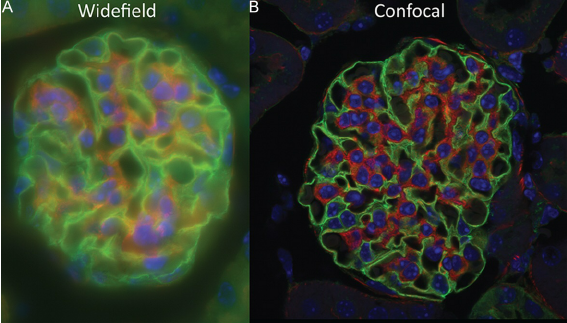
\includegraphics[width=0.8\textwidth]{figs/A-confocal-microscope-allows-you-to-do-optical-sectioning-in-thick-specimens-by-removing.png}
    \caption[A 2D image of a specimen retrieved using wide-field (left) or confocal (right) microscopy]{A 2D image of a specimen retrieved using wide-field (left) or confocal (right) microscopy \cite{specimenConfocalFig}}
    \label{fig:widevsconfocalfig}
\end{figure}

\subsection{Wide-field and confocal microscope apparatus}\label{sec:MicroAppa}
%Place this section after confocal
\begin{figure}[h!]
    \centering
    \subcaptionbox{Wide-Field Microscope\label{subfig:WFM}}{\includegraphics[width=0.28\linewidth]{figs/widefieldApparatus.jpg}}
    \subcaptionbox{Confocal Microscope\label{subfig:CM}}{\includegraphics[width=0.70\linewidth]{figs/confocalApparatus.jpg}}
    \caption[Diagrams representing the Wide-Field Microscope and the Confocal Microscope]{Diagrams representing the Wide-Field Microscope and the Confocal Microscope \cite{Sanderson-2014}}
    \label{fig:microscope_diagrams}
\end{figure}

Both wide-field and confocal microscopy are applications of fluorescence microscopy albeit with different microscope designs. The design aspects of both microscopes, seen in Fig. \ref{fig:microscope_diagrams}, are the use of filters for selecting both the excitation and emission wavelengths, the microscope objective lens and the excitation illuminant. The key components that differ are that wide-field frequently implements cube filters which both direct the excitation light to the specimen through the objective and the emission photons to the photon detectors. Filters within the cube filters select the relevant wavelengths when redirecting the light to the specimen and the detector. Conversely, confocal microscopes implement multiple adjustable, and fixed, mirrors in combination with filters. These mirrors allow the excitation laser to be directed to specific regions of the specimen and the resultant emission fluorescence reflects off of these mirrors on approach to the photon detector. The adjustment of the mirrors determines the angle at which the emission fluorescence approaches the photon detector based on the point of emission relative to the mirror angles. Confocal microscopy also uses a pinhole aperture before the photon detector which rejects photons depending on the angle at which they approach the pinhole. It is the combination of the adjustable mirrors manipulating the emission fluorescence angles with the pinhole that allows the reduction of emission fluorescence outside of the position of focus from reaching the photon detector. This position of focus can also be adjusted in depth using microscope apparatus allowing separated cross-sections through the specimen to be captured along the specimen depth. In the confocal microscope, the excitation illuminant is a precise laser as opposed to the wide-field illuminant which radiates across the whole specimen~\cite{Sanderson-2014}.\par
\textcolor{red}{This is one of the few subsections where I performed no revisions besides passing through it to check coherency. If you feel this section is unnecessary please let me know.}
\subsection{Summary}
Many aspects of fluorescence microscopy have been discussed ranging from some of the factors under which fluorophores (indicators) are selected to the decisions between the microscopy method applied. The key points covered are that different fluorophores bind to specific environments or subjects based on their chemical or biological composition; the selection of these fluorophores must consider their excitation and emission spectra to avoid overlap; confocal microscopy enables more detailed imaging with less out-of-focus fluorescence with the added option of three-dimensional imaging.
\textcolor{red}{I initially wrote this summary a year back and haven't done so for other sections. Do you think it would be beneficial to provide a short summary of a section at the end of a section or should I scrap the summaries as a whole? If I am going to keep summaries I feel I need to do it for every section out of consistency.} 

\section{Colocalization}\label{sec:coloc}
With the specimen imaged using fluorescence microscopy, as described in Section \ref{sec:fluorMicr}, mitophagy occurrence is to be measured. Through fluorescence microscopy, each of the organelle types has been separated by the selected fluorophore excitation and emission spectra such that a different colour channel can be assigned to each. Since mitophagy involves the engulfment of mitochondria by autophagosomes which fuse with lysosomes (becoming autolysosomes) it can be assumed that the overlap of mitochondria and autophagosomes (or lysosomes) would be a sufficient indicator of mitophagy. While this holds in a physiological sense, this is not guaranteed for the overlap of structures between two channels, one of which is the mitochondria channel, as that would imply that what was imaged is a perfect representation of the specimen organelles to the highest level of precision. While newer microscopy architectures and methods have increased in imaging resolution to older iterations the required resolution and precision increase as there are attempts to image smaller structures and objects with increased fidelity and detail. To compensate for this shortcoming in the image representation of the specimen a reliable framework is required to evaluate the overlap present by several factors and calculate the certainty that the perceived cross-channel overlap can be classified as colocalization~\cite{practical_guide_coloc}.\par In "A practical guide to evaluating colocalization in biological microscopy"~\cite{practical_guide_coloc} there is specific mention of two components which derive colocalization and they are co-occurrence and correlation. Co-occurrence is identical to the aforementioned overlap where the fluorescence from each channel occupies the same position in space. Correlation measures the intensities of the fluorescence between each channel relative to the distribution of these intensities over space. In combination, this results in colocalization being evaluated by not just the spatial co-occurrence of fluorescence channels in the image but also the proportion of fluorescence intensities between each channel at these regions of co-occurrence.\par While co-occurrence may be sufficient for visual evaluation of possible colocalization events it is an unreliable indicator of colocalization within the specimen as a qualitative measure of correlation is unintuitive and difficult. For this reason, there exist a number of algorithms which measure colocalization within the image region or a selected sub-region as true colocalization cannot be determined due to imaging limitations and the number of spatial characteristics describing colocalization being difficult to fully capture. Due to this many of these algorithms provide pros and cons based on the application. These pros and cons can range from intermediate values (between 1 and 0) being uncertain in interpretation, being sensitive to noise, or time-expensive iterations to converge to a reliable result~\cite{Bolte-2006}. The standard colocalization algorithms are Pearson's correlation coefficient, Manders' overlap coefficient, Manders' correlation coefficient, Costes' approach, Van Steensel's approach, and Li's approach~\cite{Bolte-2006, practical_guide_coloc}.\par These methods provide a numeric evaluation of the colocalization present in the analyzed region but due to the constraints present within these methods, they are typically applied to selected sub-regions as opposed to the full specimen image. When these regions contain multiple colocalization events these methods cannot distribute the calculated colocalization score between the events thus precise region is of greater importance to evaluate the colocalization measure of each region of co-occurrence. A recently developed method is that of Regression adjusted colocalisation colour mapping (RACC)~\cite{racc} which calculates the colocalization throughout the region (which can be the entire image) and outputs the specimen image (with both images overlaid) with a colocalization channel overlaid. This colocalization channel presents values proportional to the colocalization strength which is zero for regions without overlap but across regions of co-occurrence the provided value allows the colocalization strength to be spatially and visually mapped to these individual event locations within the specimen.
%Need to write a reduced section on Colocalization. Should be sufficient to only discuss colocalizing, RACC and briefly, BRIEFLY mention the other measurements but do not go into depth for them (RACC slightly can go into)

\section{Image preprocessing}\label{sec:image_prepro}
%Avoid going into techniques. This can be summarised as a filtering stage (containing background removal), deconvolution and thresholding. Leave the techniques for the implementation section as this is not a focal point and will be time demanding

With the specimen images acquired through microscopy, some of which are detailed in Section \ref{sec:fluorMicr}, the analysis of the features described by the image would ideally commence. As was introduced in Section \ref{sec:intro_noise}, it is not uncommon for the specimen representation captured in the image to deviate from the actual specimen due to the presence of noise, distortion or artefacts. In the context of noise, the quality of the image can be approximated as the similarity between the actual specimen and the structures of interest that may be labelled and what is described in the captured image.\par This actual specimen representation refers to the ideal visualisation of the specimen where stained structures and biomolecules of interest to the analysis are accurately differentiated as well as the size, shape and position of these captured in the image precisely reflect the matching objects in the real specimen. When there are components in the image that are not reflexive of the image then the image diverges from the specimen and the image degrades thus elements of the image causing this are referred to as degradation factors.

\subsection{Sources of interference in image quality}\label{sec:Noises} %This section needs to be reviewed fully with new understanding regarding what is of importance. We never deal with microscopic and photon noise as they form part of the background noise.

As mentioned prior, the correction of the image quality degradation is necessary for the accurate analysis of these microscopy images. The factors contributing to the degradation have been listed as distortion, noise and artefacts although there is a tentative degree of overlap between these. For clarity, the definition of distortion, noise and artefacts in the context of this research will be presented before future use.\par Distortion is the spatial deformation of the image signal such that the shape of the image signal and described features differ from the real subject. Noise can be visually described as perturbations of the captured structures in the image that reduces their clarity without presenting distinct structures (where distinct structures have shape and size similar to the structures of interest). Since noise is typically thermal or electrical in origin (from the microscope) the noise factor is applied to the image signal when captured and is applied across the entire image with the severity of this noise described as the ratio between the image signal power and the power of the noise termed as the signal-to-noise ratio (SNR). Artefacts are the last component and describe any aberration in the captured image signal such that distortion and noise could be categorized as types of artefacts. For this research artefacts will refer to visual aberrations in the image signal that are irregular and present with sizes and shapes closer to the structures of interest but typically are lacking in overall signal intensity at that focal plane. The severity of these artefacts is dependent on the similarity between them and the structures of interest and how close the average intensity of an artefact is to the average structure intensity. These artefacts originate from fluorescence that was not intended for capture (due to the occurrence of bleed-through); the fluorophore could be binding to biomolecules outside of expectation (e.g. binds to specific proteins but unexpectedly these proteins are found in both the cytoplasm and the organelle with the former being unexpected); or out-of-focus fluorescence from a currently out of depth structure has not been sufficiently reduced appearing as an artefact. This sounds similar to that of noise but rather these artefacts can originate from specimen elements that are not intended for capture yet are described, even weakly, within the image.\par With these research-specific definitions presented an overview of some of the origins of these image quality degradation factors is described below: 

\begin{itemize}
    \item \textbf{Microscope Noise}: This takes the form of Poisson noise and Gaussian noise contributed to the image signal through the photon detector by thermal and electrical noise originating from certain microscope components.
    \item \textbf{Photon Noise}: Due to the discrete particle nature of photons the quantity of photons emitted by excited fluorophores is not consistent. When this inconsistency in emission occurs there is in turn a variation quantity of photons detected by the microscope over a period of time. This culminates in the variance of the image signal strength, particularly for short imaging periods where a baseline expected photon count cannot be reliably determined to mitigate this variation. This variance visually appears as noise which is characterised in the image signal by a Poisson Distribution~\cite{Meiniel2018, PoisGauss}.  
    %\item Speckle Noise:
    \item \textbf{Microscope Diffraction}: As described in Section \ref{sec:ConstraintsMicrosc}, the fluorescence emitted by the specimen passes through an objective lens and a pinhole aperture both of which cause the photon signal, when viewed as a wave, to diffract. This diffraction induces a distortion of the image signal at the detector and can be characterized as a blurring radiating from each pixel. The severity of this distortion is relative to both the image signal conditions (e.g. emission wavelength) and the microscope apparatus (e.g. numerical aperture).
    %Need to refer to distortion here here
    \item \textbf{Background fluorescence}: As described in Section \ref{sec:ConstraintsMicrosc}, this is a broad category of fluorescence which has been unexpectedly captured and does not necessarily originate from the selected fluorophores in focus. This can contain auto-fluorescence, out-of-focus fluorescence, and bleed-through among many other possible environmental fluorescence.
    % Should refer to artefacts here in some capacity even minor
\end{itemize}

\subsection{Standard pipeline for image pre-processing}\label{subsec:pipe}
%The introduction already introduces the pipeline and preprocessing. This should be a shorter section providing greater detail and focus on the numbered list below. This will lead into the solutions section which are what are implemented in this pipeline
%Should reference Chaudhy here for a pipeline base
Specimens are imaged using microscopy to analyse and measure properties, activities, and behaviours related to the specimen. These specimens are imaged such that the visual features describing phenomena and characteristics can be measured for the appropriate analysis. As detailed in Section \ref{sec:Noises}, the reliability of these measurements is proportional to the image quality which is degraded by several factors. To restore image quality several methods can be applied which reduce the presence of these degradation factors. This phase of the image preparation before the analysis, but after imaging, during which these methods are applied is referred to as the pre-processing phase (introduced in Section \ref{sec:intro_noise}) where a number of these methods are applied sequentially. This sequential application of methods and techniques for image quality restoration is the pre-processing pipeline (introduced in Section \ref{sec:intro_prep_pipeline}) through which the output of each method feeds into the input of the next allowing the degradation reduction to compound along the pipeline. \par There are numerous different techniques which can be applied each of which addresses specific degradation factors and have conditions under which they perform optimally. It is for this reason that sequential application of methods is ideal as these techniques address different degradation factors but in the process of reducing these factors the image signal can get diminished if too aggressive (e.g. blurring structure edges during noise removal) or the performance of said techniques are sensitive to the presence of other factors. By sequentially applying these techniques preceding techniques can reduce factors while improving the conditions for proceeding techniques while proceeding techniques can compensate for the limitations of the prior techniques. For this reason, it is important to plan the techniques used and the aggressiveness at which each technique is applied to balance between image signal preservation and noise removal. For colocalization analysis (overview in Section \ref{sec:coloc}) in the context of the mitophagy research use case a high-level abstract pre-processing pipeline, based on the pre-processing employed by \cite{PipelineDecon-Chaudhry}, is presented: 
\begin{enumerate}
    \item The PSF for the image is generated based on the image metadata and the microscope used. This was mentioned in Section \ref{sec:ConstraintsMicrosc} and will be discussed in further detail in Section \ref{subsec:Decon}.
    \item Deconvolution is performed on the image utilizing the appropriate PSF. This will mitigate the distortion which occurs at the objective lens. The reason for deconvolution being applied so early will be discussed in Section \ref{subsec:Decon}.
    \item Filters and image enhancement is employed to maximize the image signal strength while diminishing, or removing, noise. Frequently employed noise removal can diminish signal across the image although more so for noise thus image enhancement restores the strength of the image signal. 
    \item Foreground and background segmentation. The removal of artefacts induced by background signals and uneven illumination that is both irregular and prominent for standard denoising to effectively mitigate.
\end{enumerate}
Further image segmentation techniques or analysis techniques would be employed after this to acquire the measurements from which to draw observations. For the mitophagy use case, these observations will typically relate to the conditions and behaviours of the imaged organelles concerning the mitophagy process. This is not definitive of all pre-processing pipelines but provides an example of the sequential order in which these methods are applied for effective image preparation.

\subsection{Overview of the methods to restore image quality}\label{sec:overview_preproc_methods}
As discussed in Section \ref{subsec:pipe} prior, several techniques are applied sequentially to the image to restore the image quality. These techniques will be categorized (for this research) by the effect they have on the image. The groups will be deconvolution, denoising, image enhancement and thresholding. 

\subsubsection{Deconvolution}\label{subsec:Decon}
%Make sure the relation of the PSF to the NA of the objective and the emission wavelength is important as that is the wavelength that the dispersed spectrum is centred around and is important to reconstruct the original channel fluorescence.
During the imaging process, there is some degree of expected blurring of the image due to diffraction. This was described in detail in both Sections \ref{sec:ConstraintsMicrosc} and \ref{sec:Noises} where diffraction is the phenomenon where light scatters after passing through an aperture leading to the fluorescence spreading from singular points. This spread is more visible when it originates from brighter points thus structures with strong image signals present more prominent spreads which appear as blurry regions surrounding the original structure. This is problematic as this distorts the actual spatial representation of the imaged objects as they may appear larger than they are and the overlapping of these blurred regions can obfuscate edges and fine details thereby reducing the image quality. A technique known as deconvolution can be applied to the image after imaging which works to reverse the diffraction phenomenon but this requires the diffraction pattern for the image to be known and it is for this reason that overlap between diffraction blurs can interfere with effective reconstruction.\par The diffraction pattern can be determined in several ways but a convenient and effective method is to determine the theoretical diffraction pattern by calculating the PSF. The PSF is a mathematical model of the diffraction pattern that while lacking the nuance of the actual pattern is similar enough for effective deconvolution. The PSF calculation considers several imaging and fluorophore properties such as the relationship between the image pixel size to real distance in nm, the NA, the emission wavelength, the refractive index, the distance between lateral sections in 3D images and the microscope optical model among other properties~\cite{psfgen} with an example of a generated PSF shown in Figure \ref{fig:psf_example}.
\begin{figure}
    \centering
    \subcaptionbox{First PSF slice\label{subfig:first_psf}}{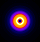
\includegraphics[width=0.27\linewidth]{figs/ch2figs/psf1.png}}
    \subcaptionbox{Second PSF slice\label{subfig:second_psf}}{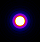
\includegraphics[width=0.27\linewidth]{figs/ch2figs/psf2.png}}
    \subcaptionbox{Third PSF slice\label{subfig:third_psf}}{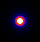
\includegraphics[width=0.27\linewidth]{figs/ch2figs/psf3.png}}
    \caption[PSF example for a 6 slice 3D image]{PSF example for a 6 slice 3D image. The PSF is mirrored between the first three and last three slices thus only the first three are shown and the order is inverted for the next three. The slices (\subref{subfig:first_psf})-(\subref{subfig:third_psf}) are ordered by depth where the later in the order the deeper the slice.}
    \label{fig:psf_example}
\end{figure}
\par In the theoretical pipeline described in Section \ref{subsec:pipe} the first step is to determine the PSF and the second is to apply deconvolution after which further processing can be applied. To justify this order first a simple algebraic representation of the captured image in relation to the blurring is shown~\cite{6505824, DeconLab2}:
\begin{equation}\label{eq:blurAdded}
    G(x,y) = F(x,y)*S + \eta(x,y)
\end{equation}
Where $G$ is the captured distorted image, $F$ is the original undistorted image signal, $S$ is the representation of the diffraction and the additive white noise is represented by $\eta$. The additive white noise is usually Poisson/Gaussian and originates from electrical or thermal energies in the microscope detector and apparatus. From \ref{eq:blurAdded}, the culprit of the distortion can be seen as $S$ which is also the PSF and the original image $F$ is convolved with the PSF to result in the distorted captured image. To reconstruct the original image $F$ a deconvolution operation needs to be applied with the appropriate PSF to `reverse' the diffraction effect of the microscope pinhole.\par
\begin{equation}\label{eq:psf_added}
    F(x,y) = G(x,y)*H(S^\ast)
\end{equation}
Where $H()$ is the deconvolution function and $S^\ast$ is the determined PSF for the image. Depending on the method by which the PSF is calculated, and when, the selection of what algorithms to apply to the image before deconvolution is significant. Operations that change the image signal, particularly in a non-linear or adaptive local approach such as Gaussian blurring, can lead to changes in the dispersion of the image signals within the image and thereby change the properties of the blur. If the PSF is generated so that these adjustments can be compensated for then this may be of little concern but if the PSF cannot do so then applying other algorithms before deconvolution could introduce unexpected outcomes and risks.\par Regarding the additive white noise, it is not uncommon for deconvolution algorithms to also remove noise~\cite{PipelineDecon-Chaudhry} and since the additive white noise is theoretically independent of the image signal distortion then denoising algorithms targeting solely the additive white noise could be applied with minimal issue.\par There are multiple deconvolution algorithms which can be used such as Richardson-Lucy, Richardson-Lucy Total Variation, Tikhonov Regularization Inverse Filter, Tikhonov-Miller and Regularized Inverse Filter to name a few~\cite{DeconLab2}. The two primary groups of deconvolution algorithms are iterative methods, such as Richardson-Lucy, and inverse methods, such as Tikhonov Regularization Inverse Filter. In Figure \ref{fig:deconvolution_showcase} the effects of deconvolution are shown with a comparison of before and after the application. The pre-deconvolution image (Fig. \ref{subfig:preDecon}) shows how the diffraction induces a blurred region distorting the perceived volume and shape of structures in the image as was discussed prior.

\begin{figure}[h!]
    \centering
    \subcaptionbox{Specimen image pre-deconvolution\label{subfig:preDecon}}{\stackinset{r}{}{t}{}{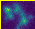
\includegraphics[width=0.1\linewidth, cframe=orange 2pt]{figs/ch2figs/Cropped_before_decon.png}}{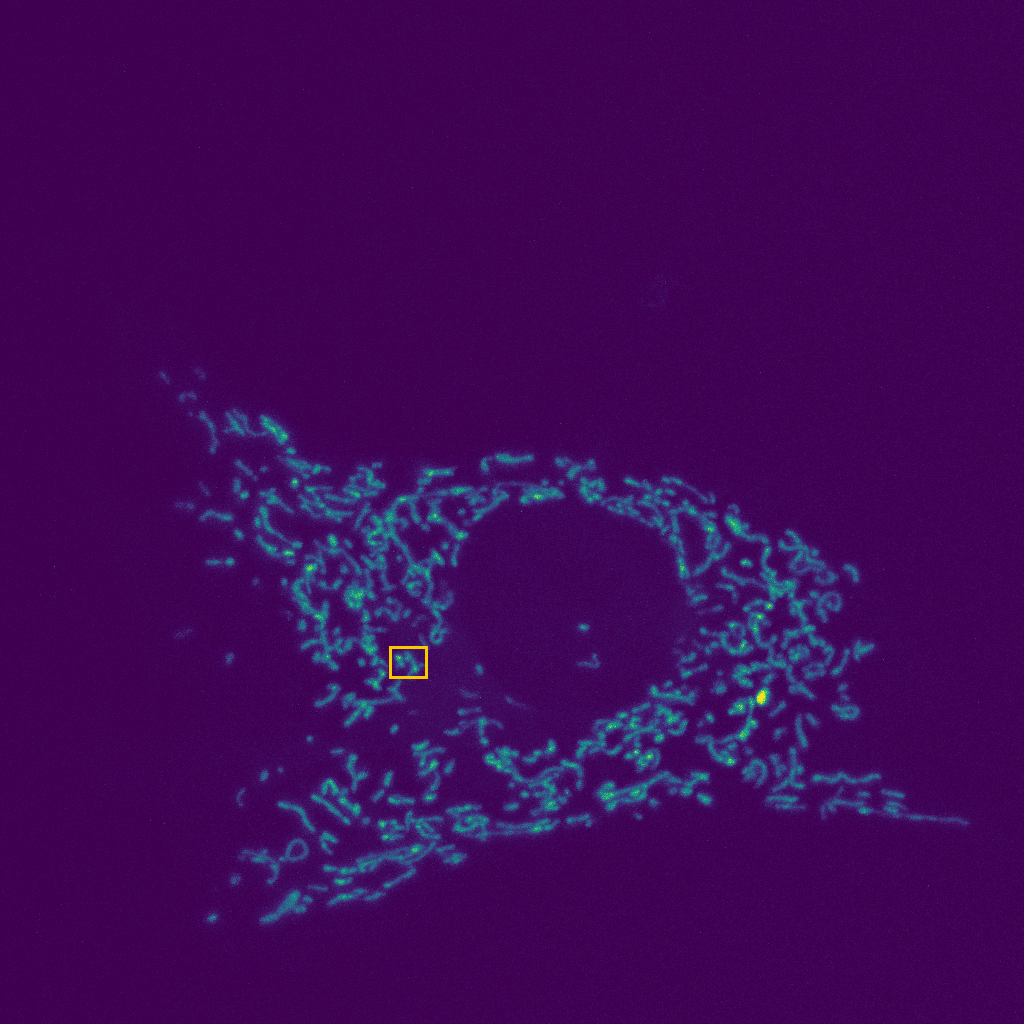
\includegraphics[width=0.49\linewidth]{figs/ch2figs/MAX_N1CCCP_1C=1_raw.png}}}
    \subcaptionbox{Specimen image post-deconvolution\label{subfig:postDecon}}{\stackinset{r}{}{t}{}{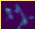
\includegraphics[width=0.1\linewidth, cframe=orange 2pt]{figs/ch2figs/Cropped_after_decon.png}}{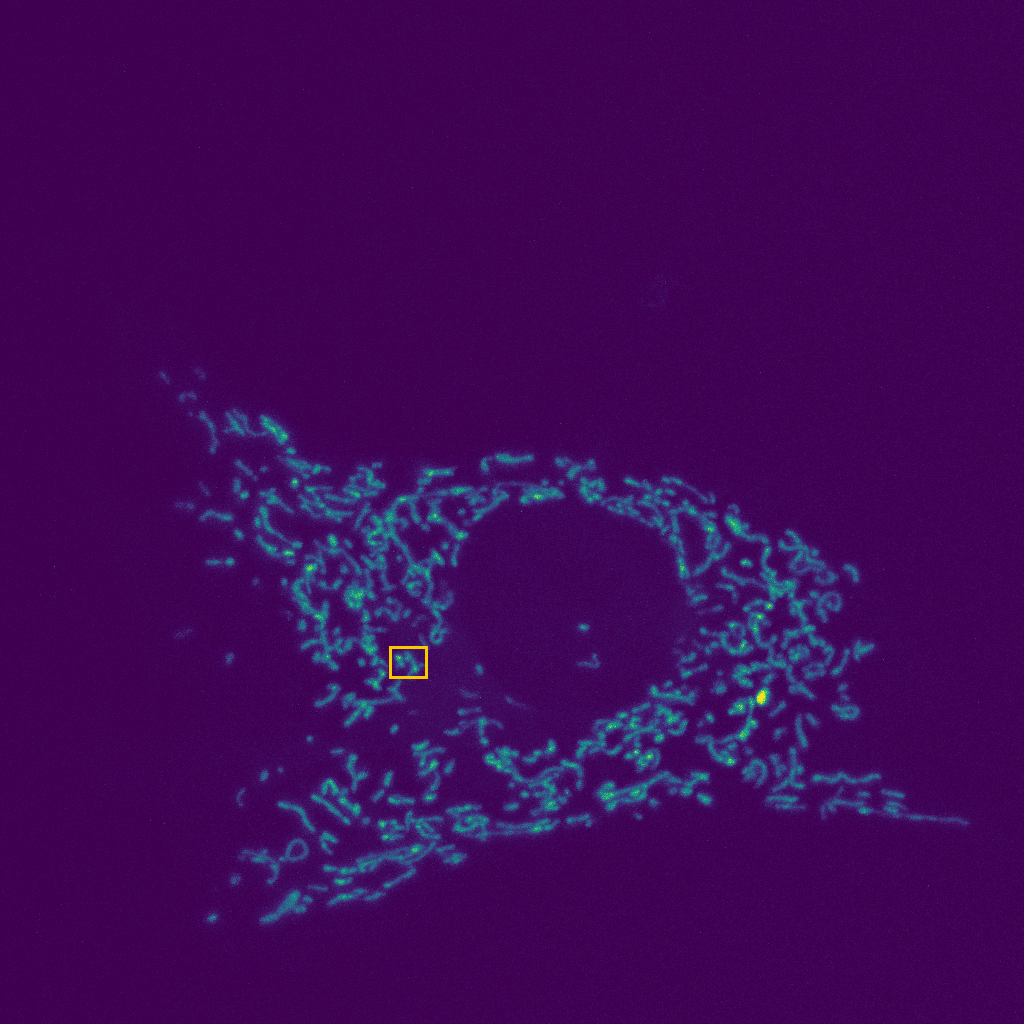
\includegraphics[width=0.49\linewidth]{figs/ch2figs/MAX_N1CCCP_1C=1_raw.png}}}
    \caption[Showcase of the effect of deconvolution on specimen images]{A maximum intensity projection of a specimen image is shown to compare \subref{subfig:preDecon}) pre-deconvolution and \subref{subfig:postDecon}) post-deconvolution. A region of interest that is zoomed-in is shown in the top right corner of each respective figure.}   
    \label{fig:deconvolution_showcase}
\end{figure}

\subsubsection{Denoising}
Denoising methods are transformations applied to the image to mitigate the presence of noise within the image. As detailed in Section \ref{sec:Noises}, regarding the degradation factors definitions, noise is generally expressed in the image as a global presence throughout the image which reduces the clarity of the features but typically does not generate new distinctive features. To clarify this, noise induces fluctuations in the amplitude of the image signal centred around the original signal and while these fluctuations are randomly distributed throughout the image they still follow certain `rules'. The fluctuations of individual pixels occur independently of other pixels yet the sign (positive or negative) and amplitude of all noise-based fluctuations across the image are drawn from the same distribution~\cite{bioimage_book}. There can be multiple noise fluctuations, with different origins, that compound in the resultant effect on the image pixels but the distributions from which these are drawn can be identical or different between different noise distributions. In an ideal situation, it may be possible to estimate the distribution of the noise from the image histogram but the compounding of other degradation factors on the image signal result in this being quite difficult for real image signals.\par Due to this methods that can mitigate the impact of the noise independent of knowing the noise distribution are necessary. These techniques are composed prominently of filter methods which are applied to pixel neighbourhoods and apply a filter operation. The filter operations can be standard mathematical operations, such as the median or mean of the neighbourhood, where the calculated value is applied to the pixel the neighbourhood is centred on. Irrespective of the exact filter method applied a consistent characteristic of denoising outputs is the smoothing of the image as can be seen in Figure \ref{fig:denoising_example} where the Sigma filter~\cite{sigma_filter}. As mentioned prior, many of these methods apply an operation to a pixel which adjusts the value based on the surrounding pixels thus reducing the variance within these neighbourhoods.\par While the discussion has been constrained to finite neighbourhoods there are also techniques which consider all pixels for the operation but the contribution of each pixel is relative to the distance from the pixel to be adjusted. This reduction in variance in image regions is fine for those already expressing a low variance but image features like edges are expressed by the relatively high variance localized around the edge. It is for this reason that excessive smoothing through denoising is detrimental for features expressed by high local variances limiting the quantity of denoising that can be applied~\cite{sigma_filter}. Likewise, even image regions that express limited variance may describe a feature yet excessive smoothing can eventually remove the boundary between the background and the objects to be analyzed. For this reason, denoising does have an upper limit on its application of it based on the noise level being too strong or the image signal being too weak. There do exist denoising methods optimized for edge preservation such as the Sigma filter~\cite{sigma_filter} but these, among the numerous other denoising methods, will not be explored in further detail for this work.

\begin{figure}
    \centering
    \subcaptionbox{Prior to denoising\label{subfig:before_denoise}}
    {\stackinset{r}{7pt}{t}{1pt}{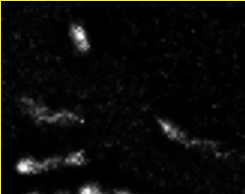
\includegraphics[width=0.15\linewidth, cframe=orange 0.5pt]{figs/ch2figs/Cropped_before_sigma.png}}{
    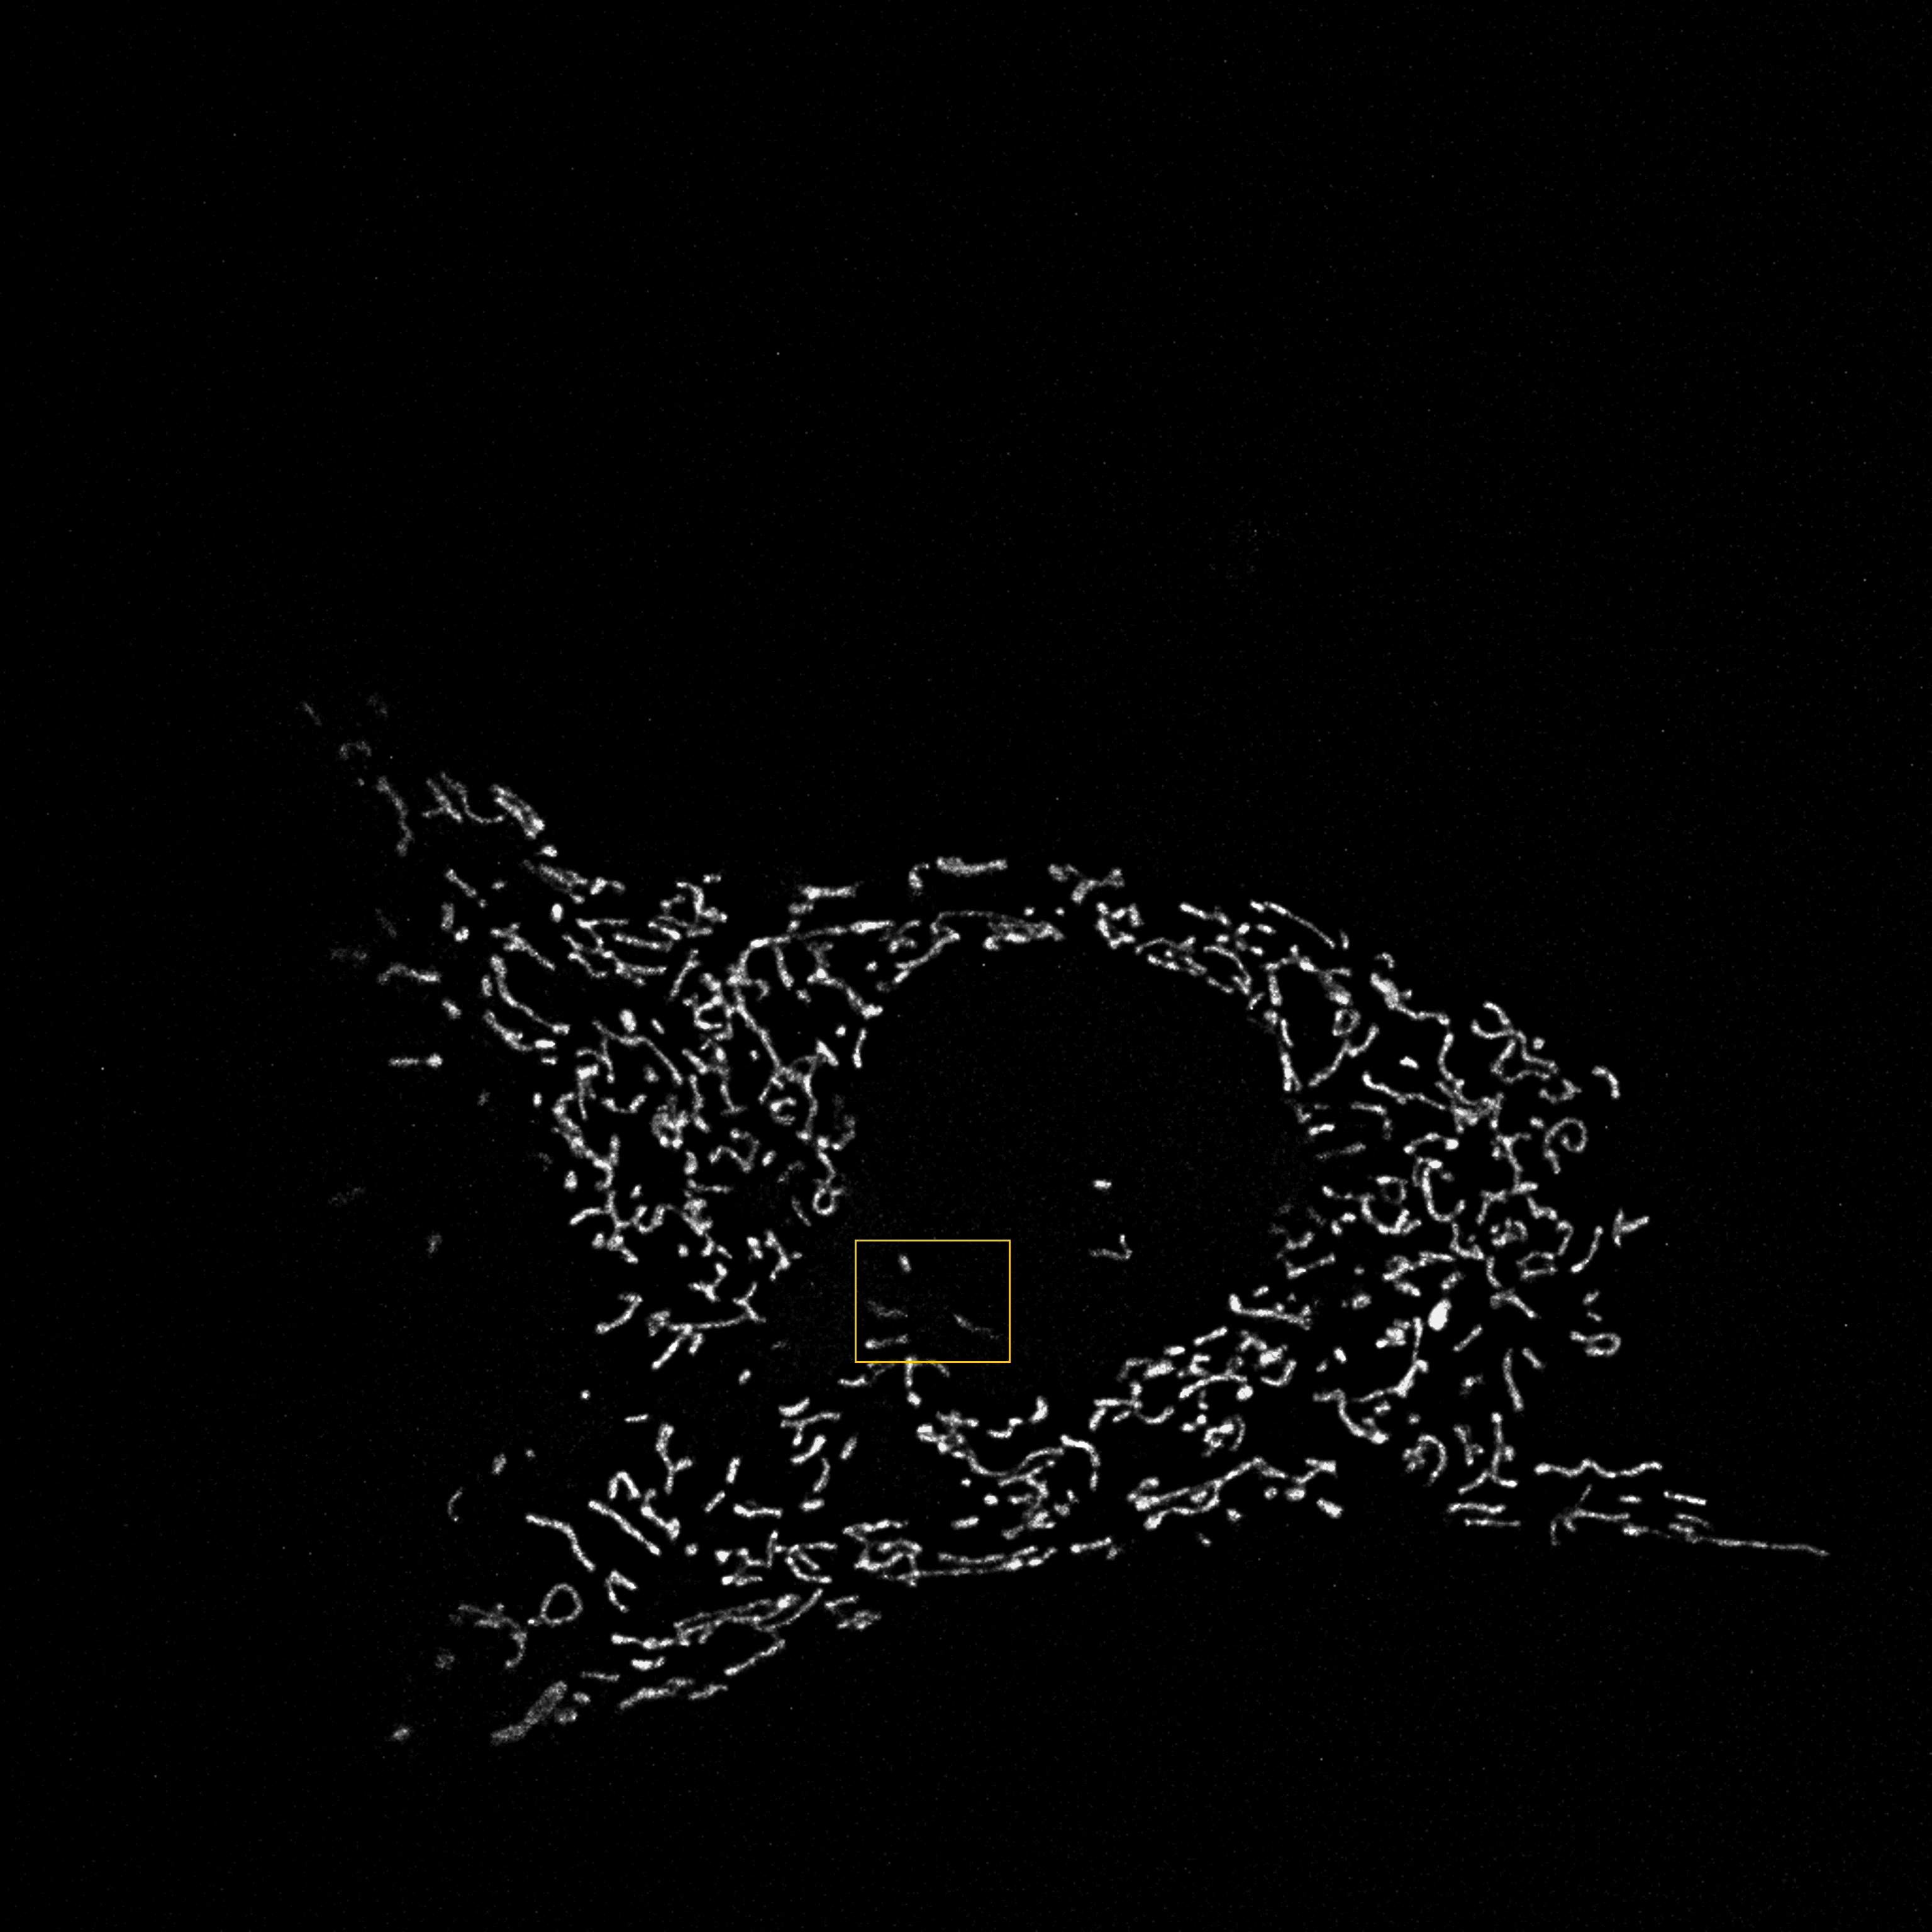
\includegraphics[width=0.48\linewidth]{figs/ch2figs/MAX_N1CCCP_1C=1_background_subtract.png}
    }}
    \subcaptionbox{After denoising\label{subfig:after_denoise}}{
    \stackinset{r}{3pt}{t}{1pt}{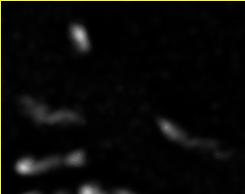
\includegraphics[width=0.15\linewidth, cframe=orange 0.5pt]{figs/ch2figs/Cropped_after_sigma.png}}{
    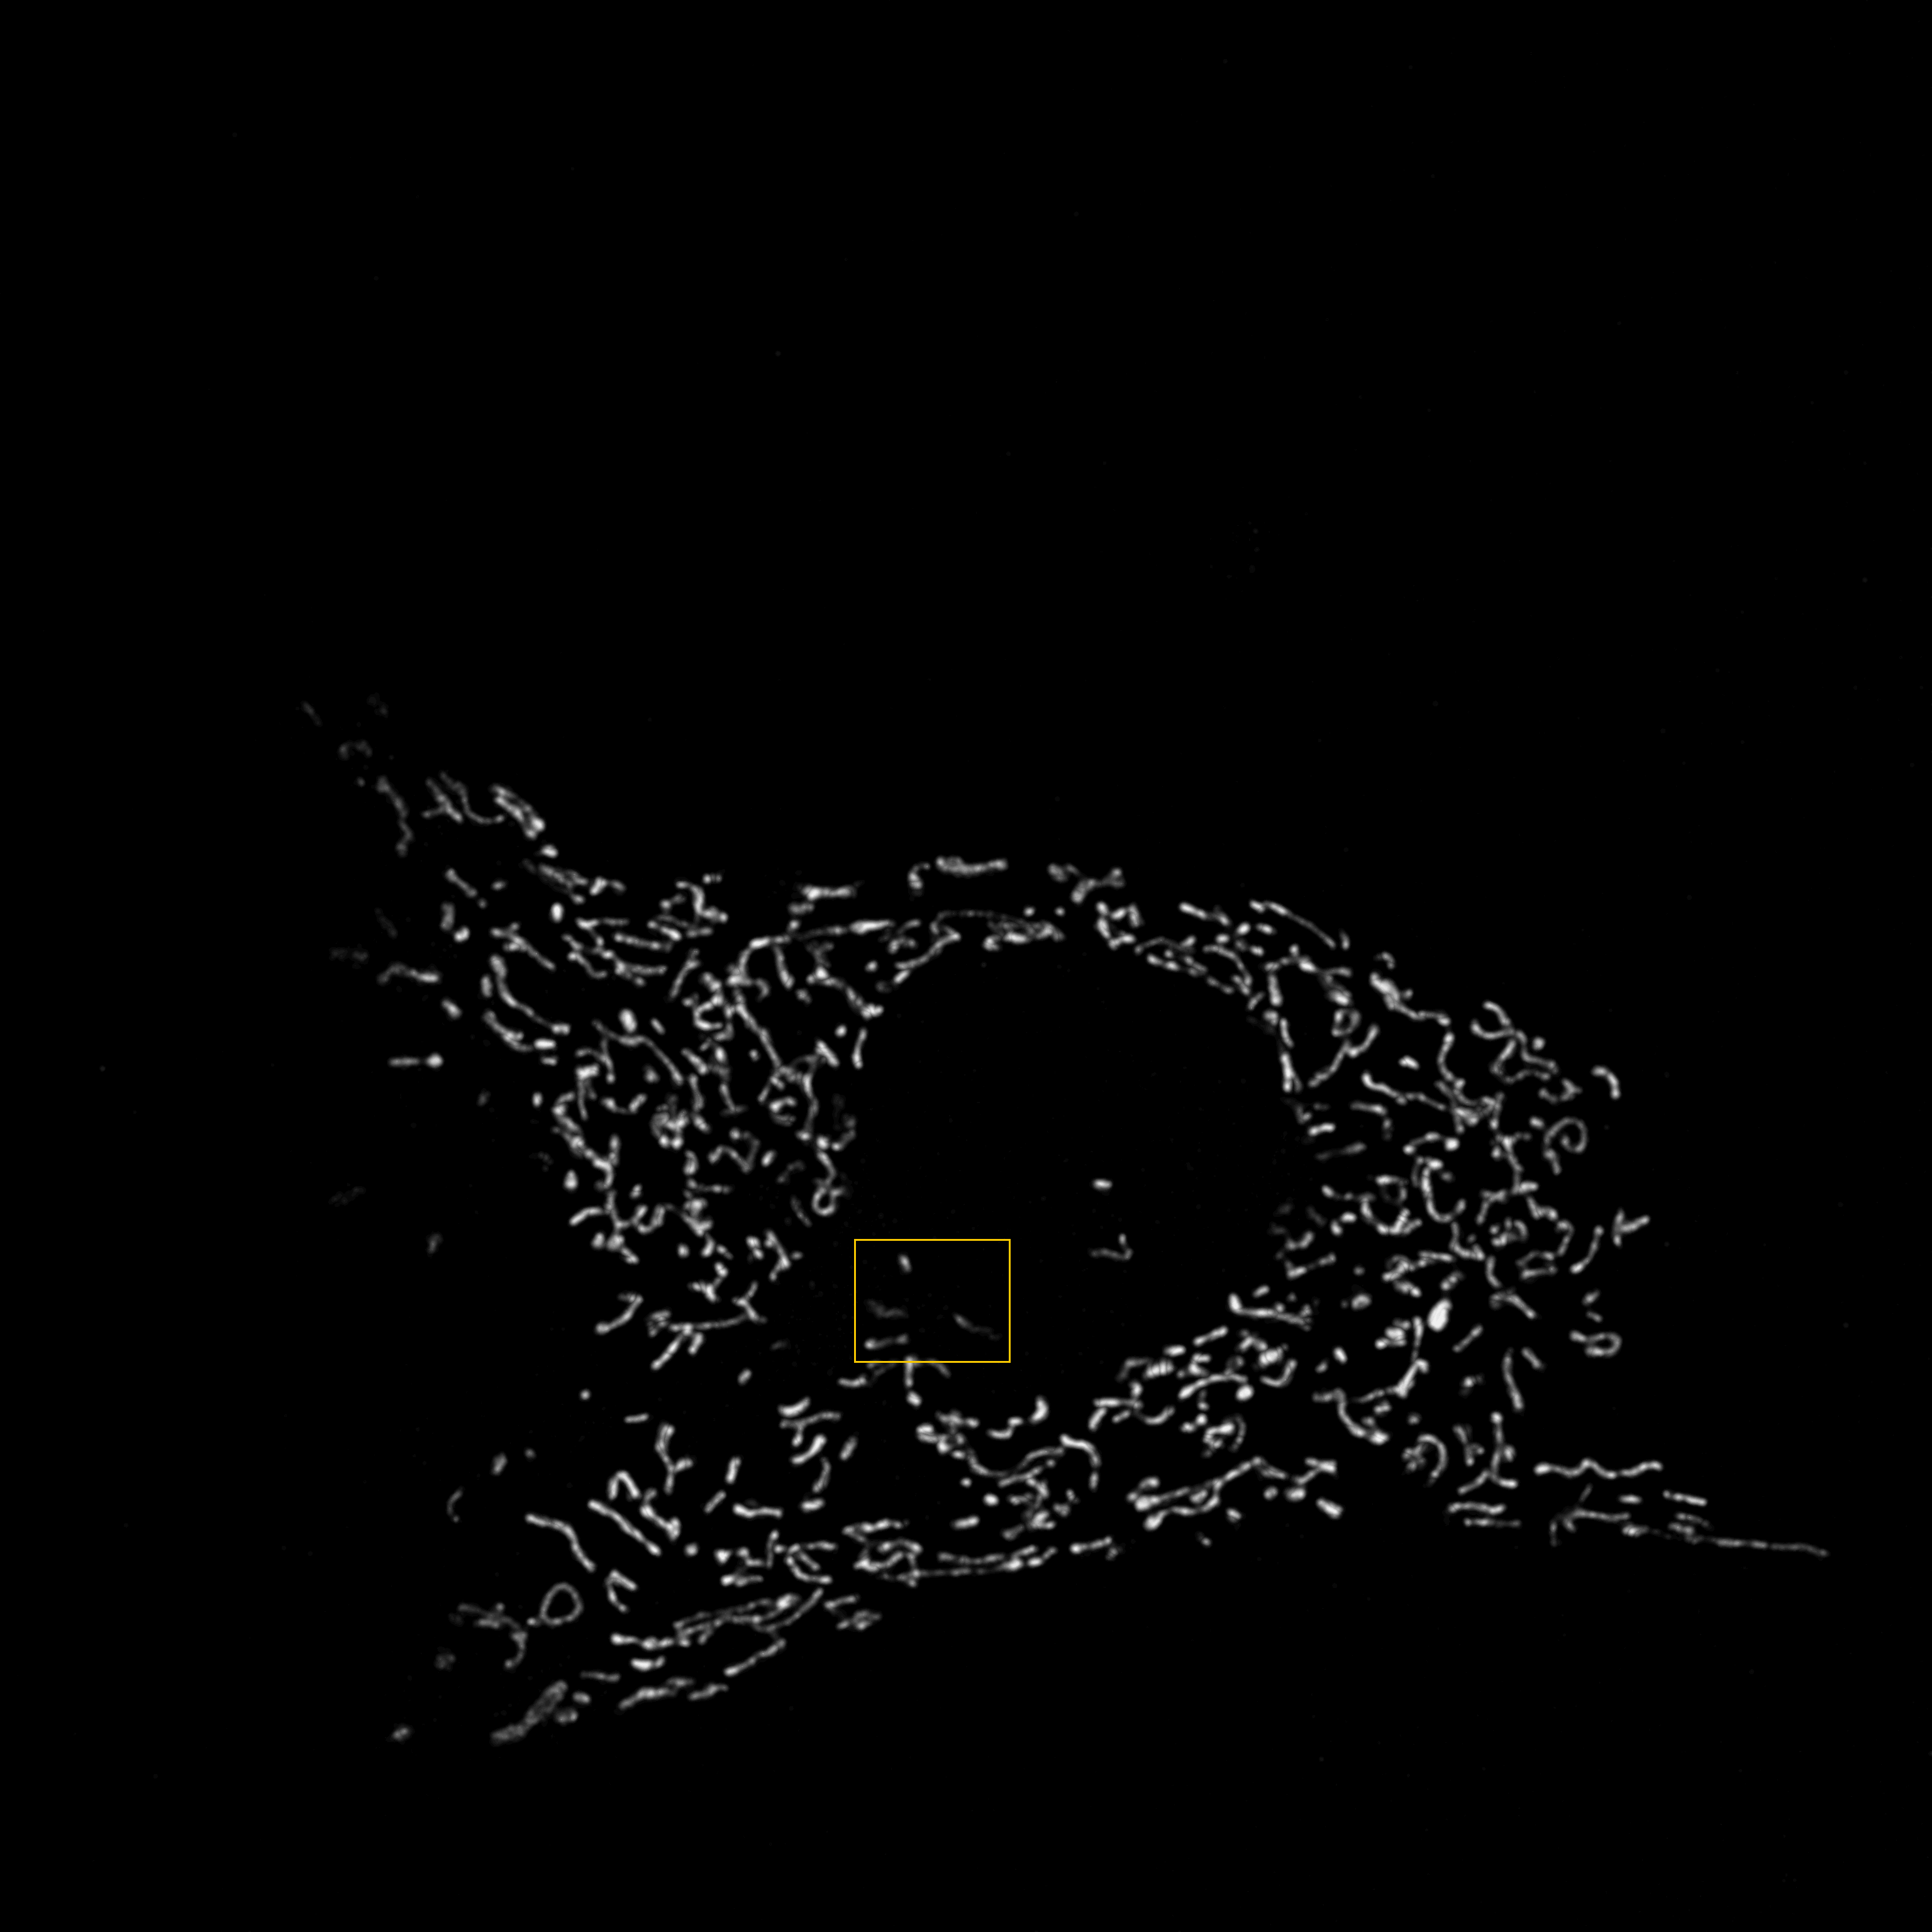
\includegraphics[width=0.48\linewidth]{figs/ch2figs/MAX_N1CCCP_1C=1_sigma_filter.png}}}
    \caption[Visual showcase of the effect of filtering on a maximum intensity projection image]{The effect of filtering on a mitochondria sample with before (\subref{subfig:before_denoise}) and after (\subref{subfig:after_denoise}). The sample images are maximum-intensity projects flattened from 3D with a region of interest bordered with an orange frame with a zoom-in at the top-right}
    \label{fig:denoising_example}
\end{figure}

\subsubsection{Image Enhancement}
While denoising methods are optimal for removing consistently present random fluctuations in pixel intensity across the image they are not designed to improve image signal strength or correct uneven signal distributions throughout the image which do not describe image features such as object edges and the region of pixels composing the body of the object. Object bodies are typically composed of pixels within a bounded range (excluding outliers) with the lower bound being of a magnitude greater than the background with the brighter pixels closer to the object centre or clustered around it. What is important is that image enhancement is easier to characterise by two components: firstly, the goal of it is to amplify the presence of both objects in the image and features describing said objects, like edges, and, secondly, while all image enhancement methods aim to enhance the image how this is done less consistent than other method types as it improved clarity and differentiation of objects from the background.\par
Before exploring the behaviour of image enhancement techniques the clarity and differentiation regarding image objects will be detailed for this context. Image objects have a body, described prior, surrounded by an edge which is in contrast to the pixels surrounding it whether those belong to some other object or the background. The contrast of the object edges is crucial to determine the boundaries of objects particularly when there are overlapping objects as insufficient contrast may lead to objects being incorrectly joined. The object body contrast does not need to be as large as the edges but must still contrast with the background as background regions in the object body could be cavities. For this reason, object differentiation is dependent on the size of the gap between the brightness of pixels composing the object and those composing the background while, in this context, the clarity is dependent on the brightness resolution of the image which can be viewed as the minimum and maximum pixel values of the image excluding outliers (outer values with relatively few pixels attributed to them) as a lower brightness resolution provides a more limited range within which to separate the object and background pixels. This also requires the background to be consistent as it is supposed to be the lowest brightness level in the image as it describes pixels where no fluorescence was localised in the actual specimen. These methods can range from contrast stretching to correcting uneven illumination. Contrast stretching can target either the whole image or localised regions within which to enhance the contrast present which is beneficial for contrast-dependent features such as detecting the edges of objects. 
Uneven illumination across the image is characterized by changes in the brightness of the pixels across the image that do not describe any objects as object edges or bodies. This change can appear to be homogeneous relative to the object sizes and interfere with the contrast required for differentiation. Due to this, methods correcting uneven illumination attempt to normalize the brightness of regions based on how low the variance within that region is i.e. brightness is lowered for homogeneous regions with low contrast while high contrast regions remain.\textcolor{red}{I struggled a bit with describing the correction of uneven illumination. While I feel my idea of it is correct the explanation feels a bit difficult. If you have any advice for simplifying it or what should be corrected in the explanation would be appreciated.} An example of correcting uneven illumination across the background is the rolling ball algorithm~\cite{rolling_ball} while an example of contrast enhancement is seen in ``Contrast limited adaptive histogram equalization''(CLAHE)~\cite{clahe}.

\begin{figure}
    \centering
    \subcaptionbox{Intensity image of the specimen prior to CLAHE\label{subfig:middleslice_noclahe}}{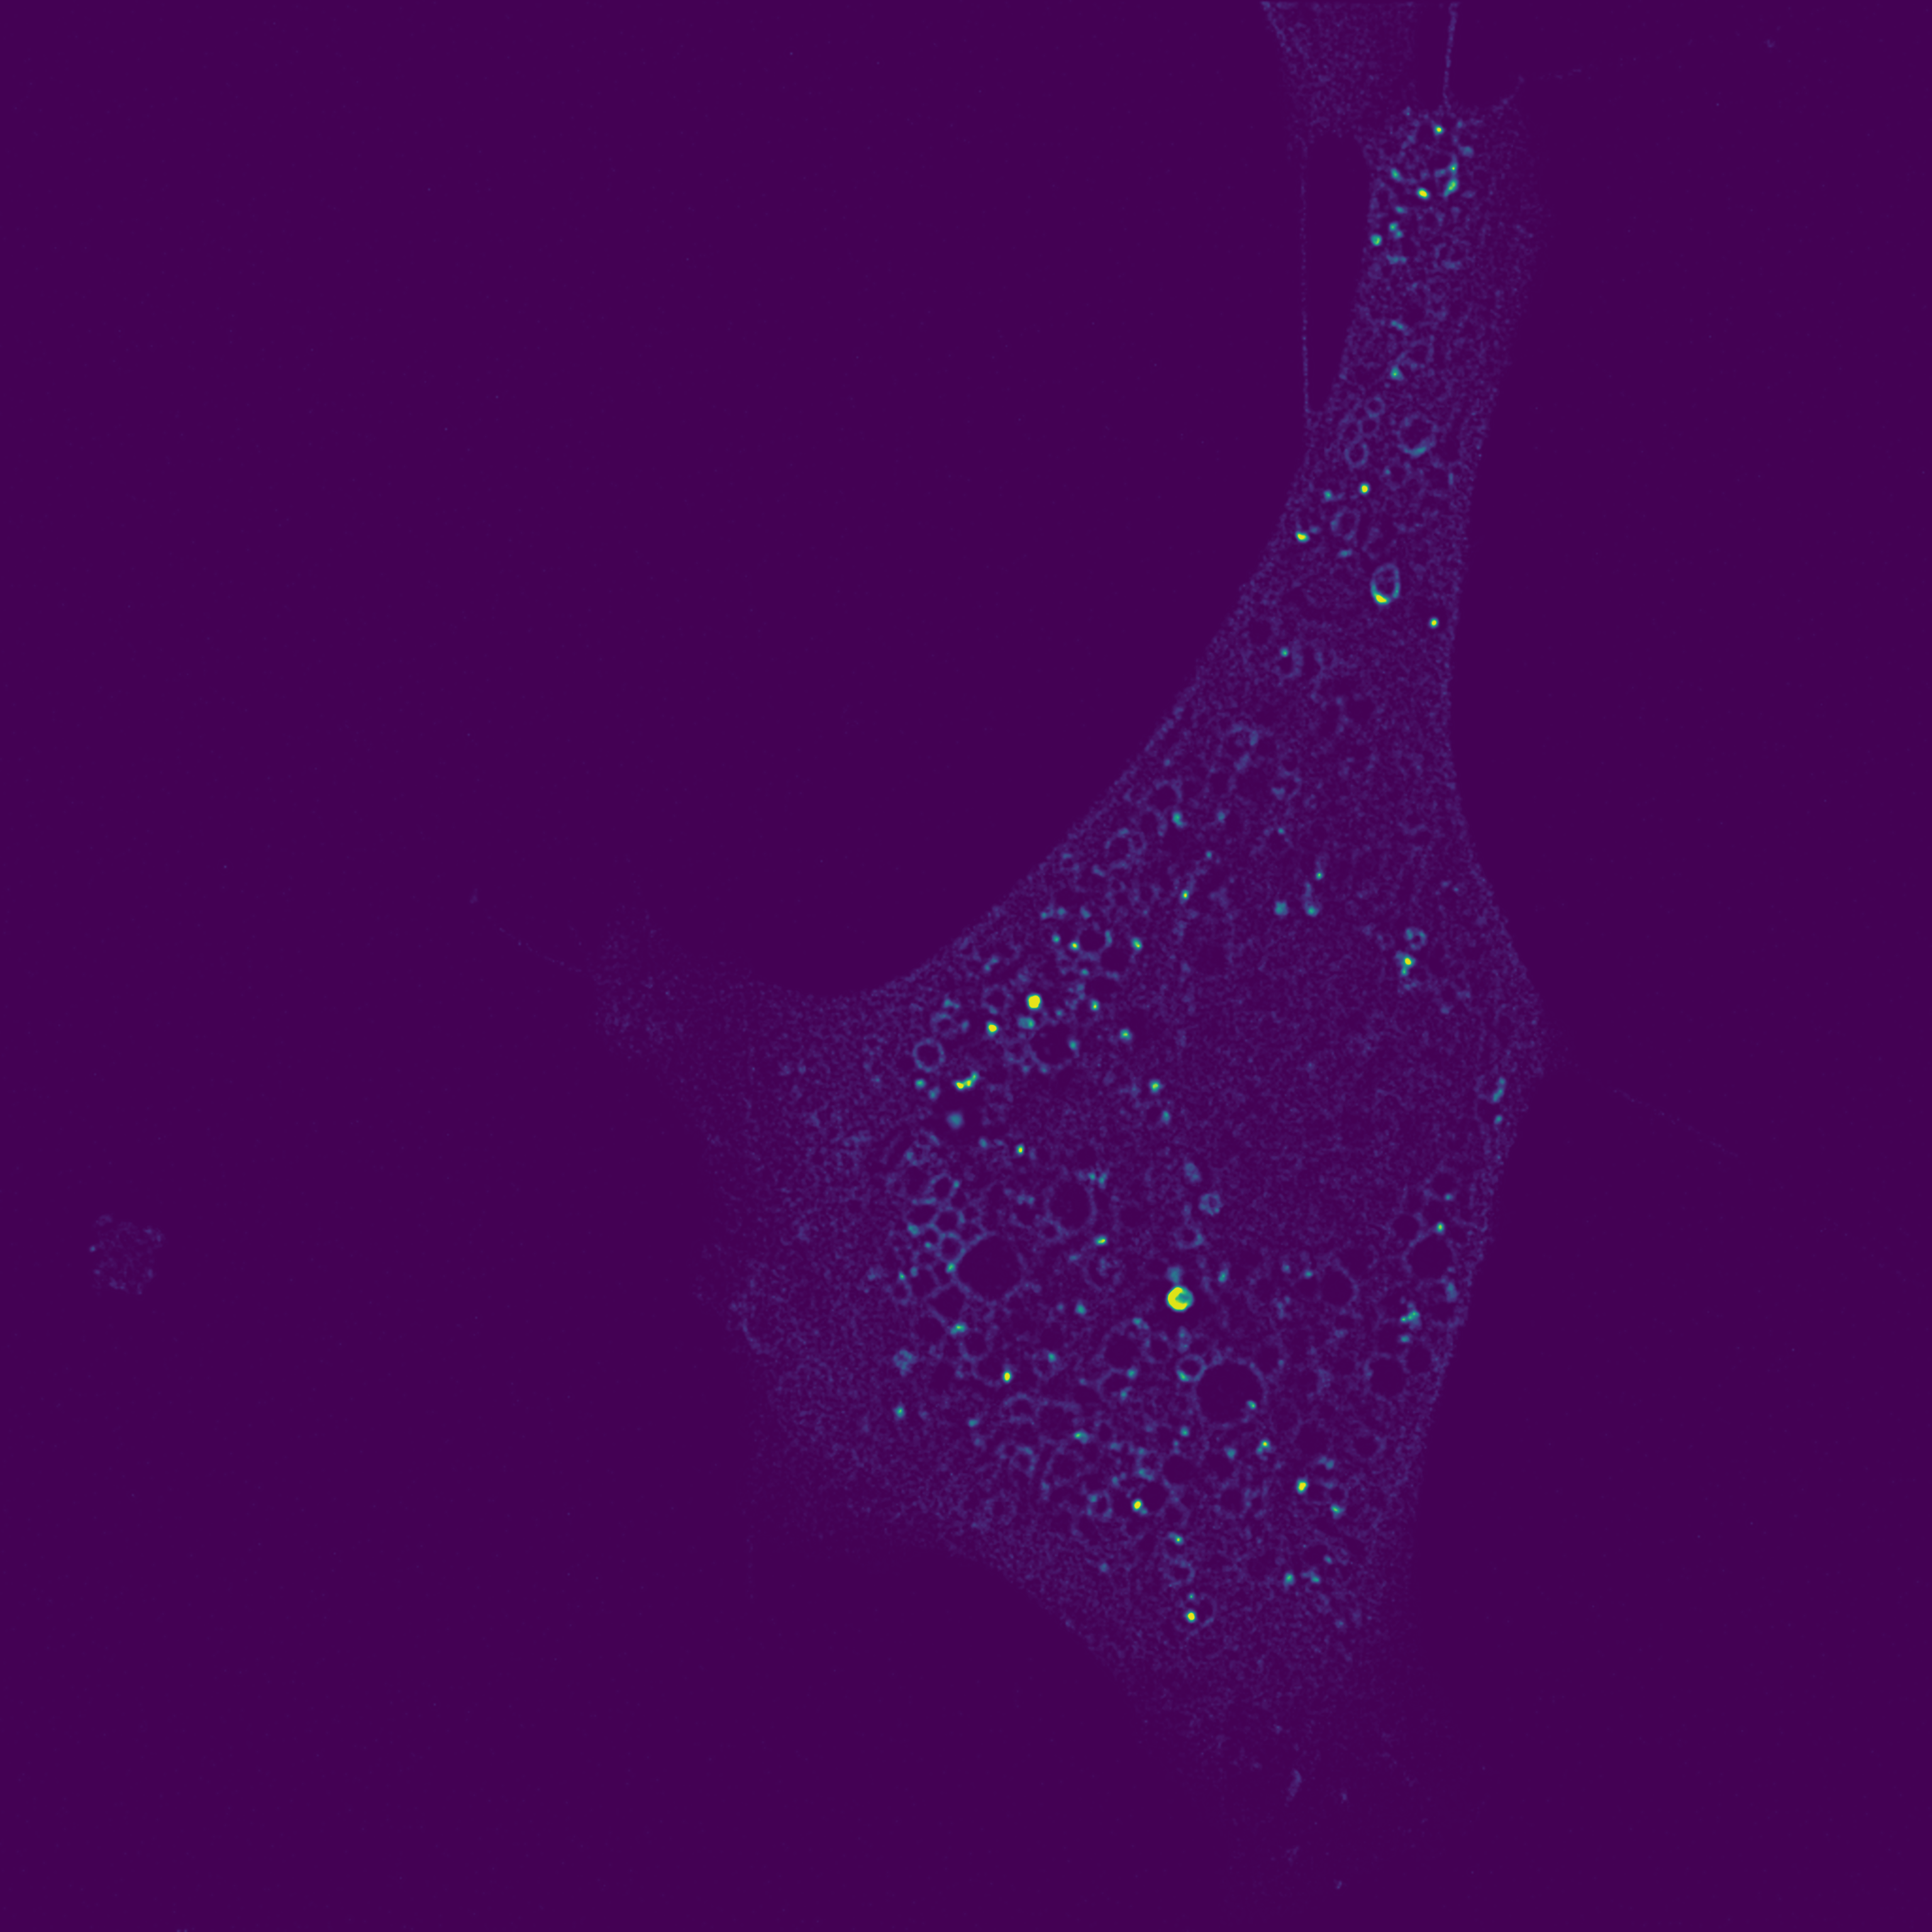
\includegraphics[width=0.49\linewidth]{figs/ch2figs/N2Con_3C=0T=0_middleslice_bs.png}}
    \subcaptionbox{Intensity image of the specimen after CLAHE\label{subfig:middleslice_clahe}}{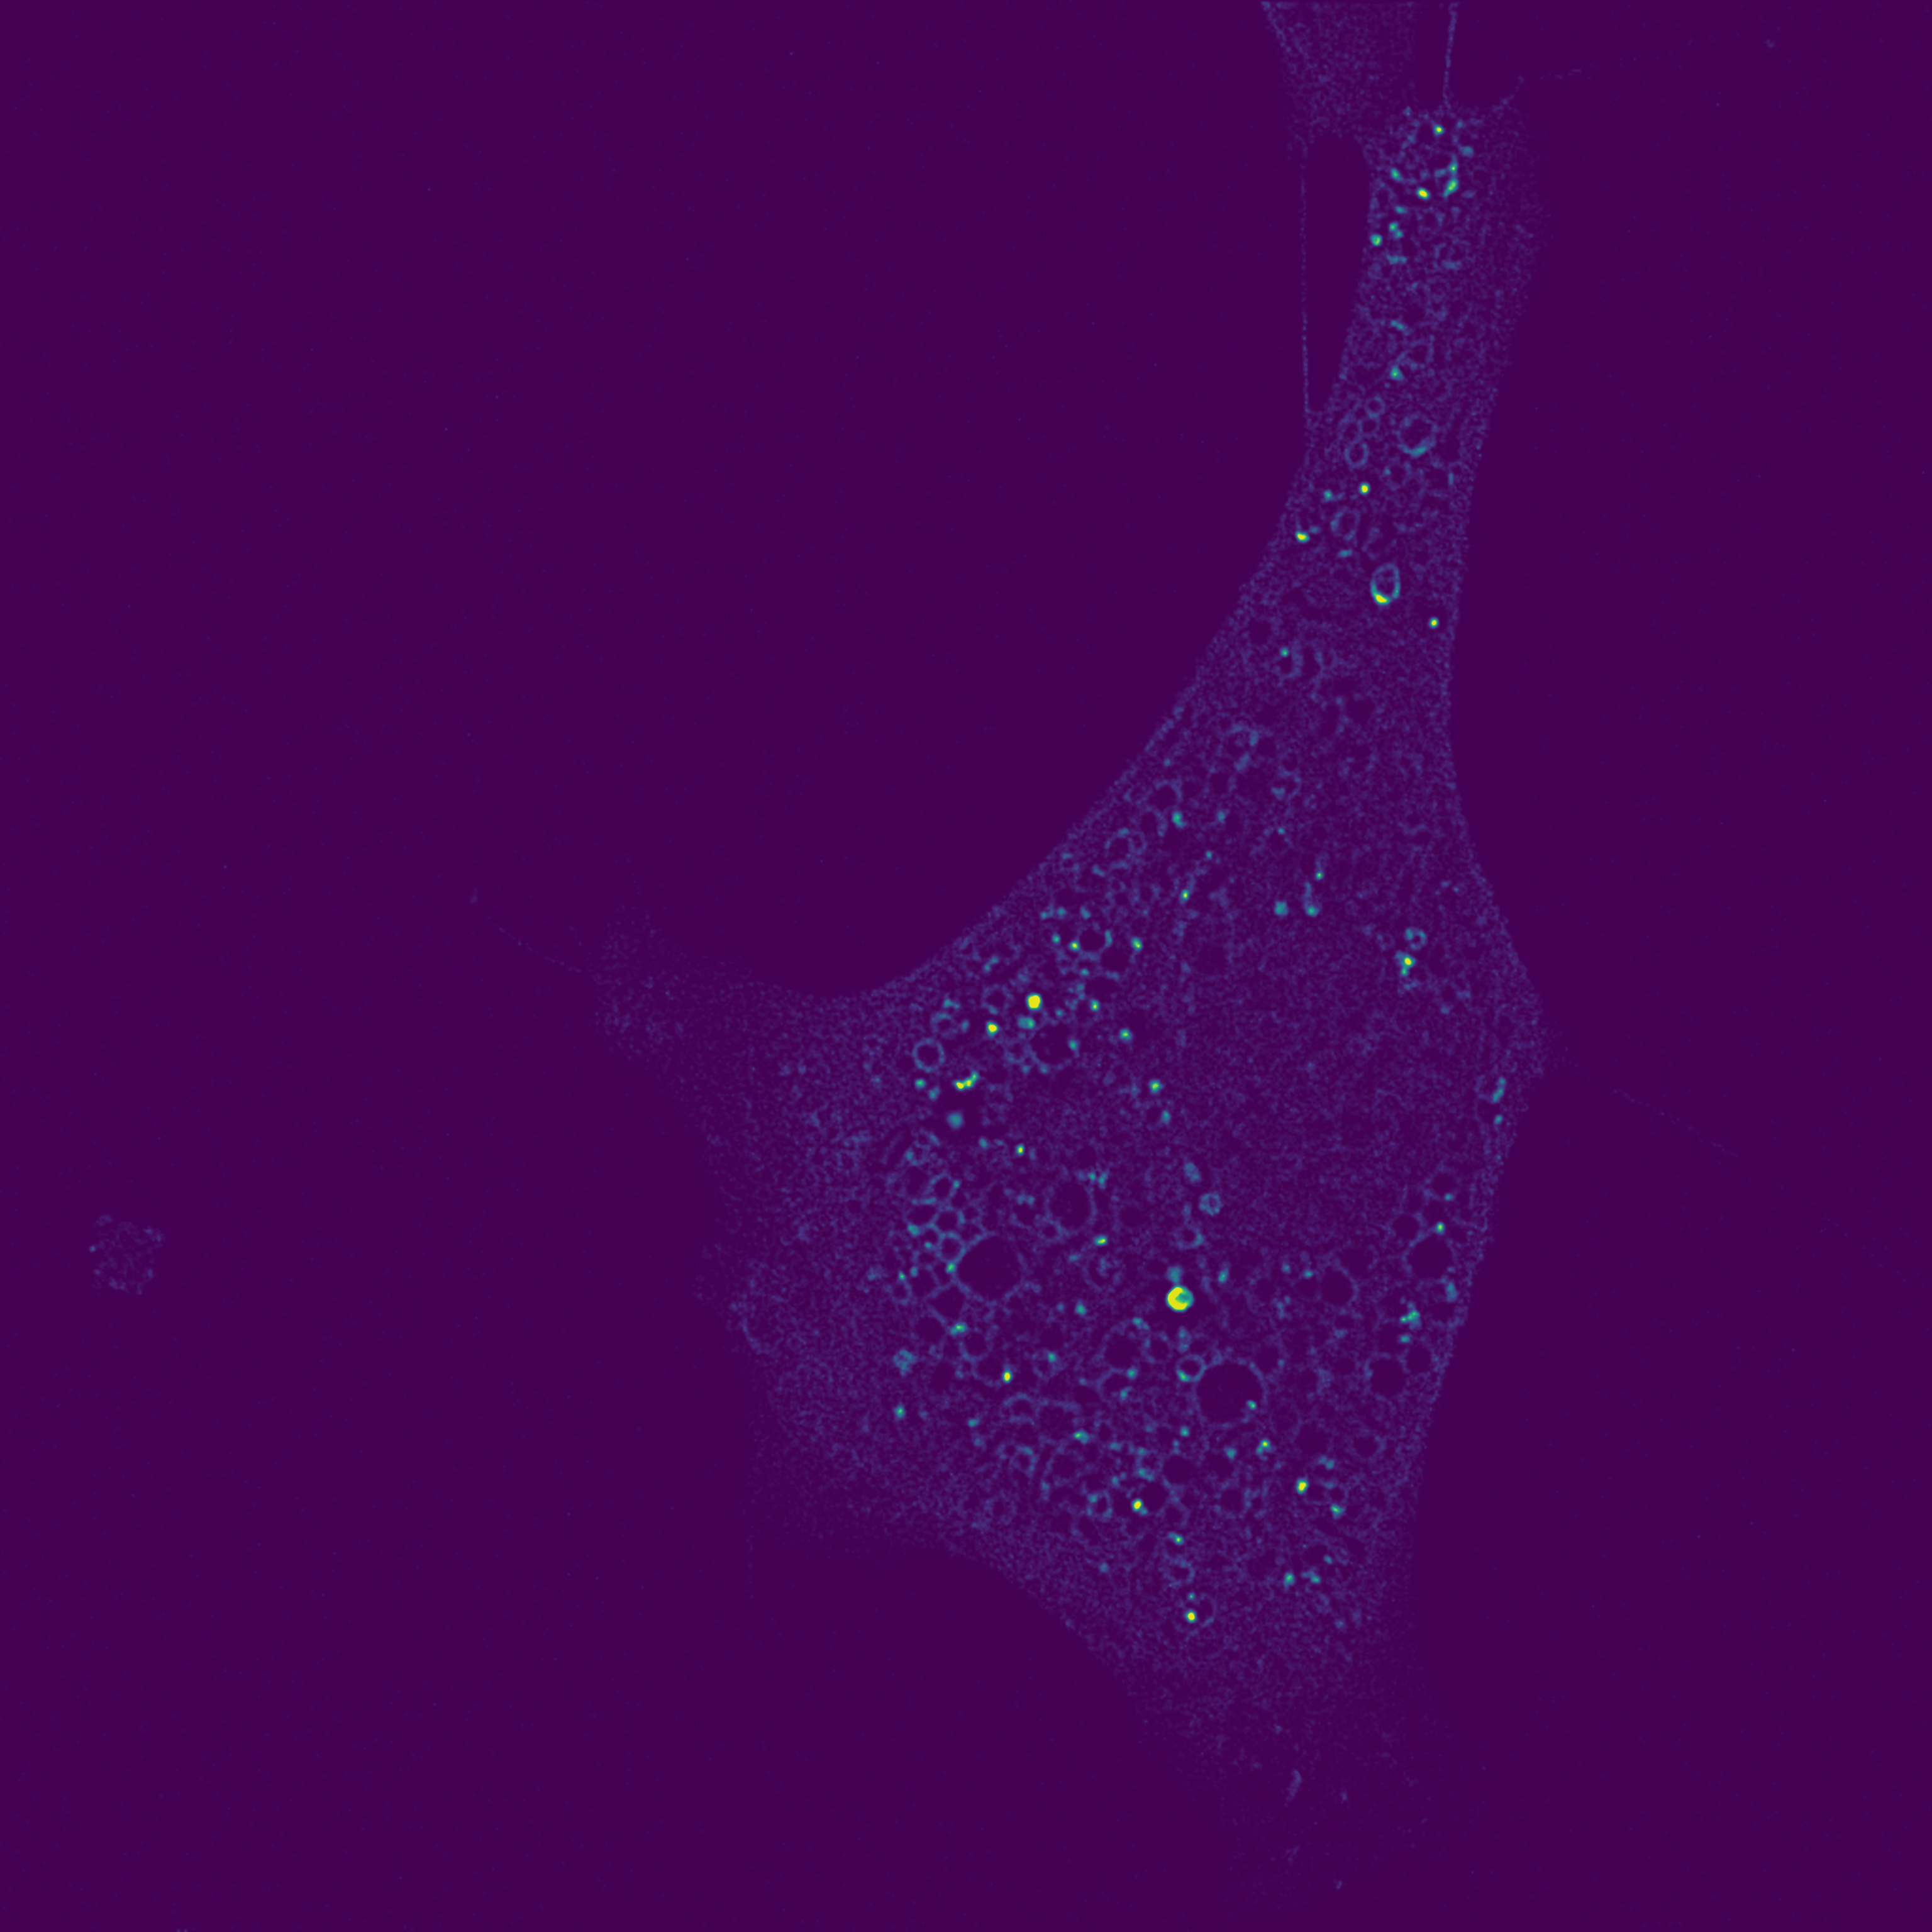
\includegraphics[width=0.49\linewidth]{figs/ch2figs/N2Con_3C=0T=0_middleslice_clahe.png}}
    \subcaptionbox{Binarised image after the Otsu threshold has been applied to Image \subref{subfig:middleslice_noclahe})\label{subfig:otsu_before_clahe}}{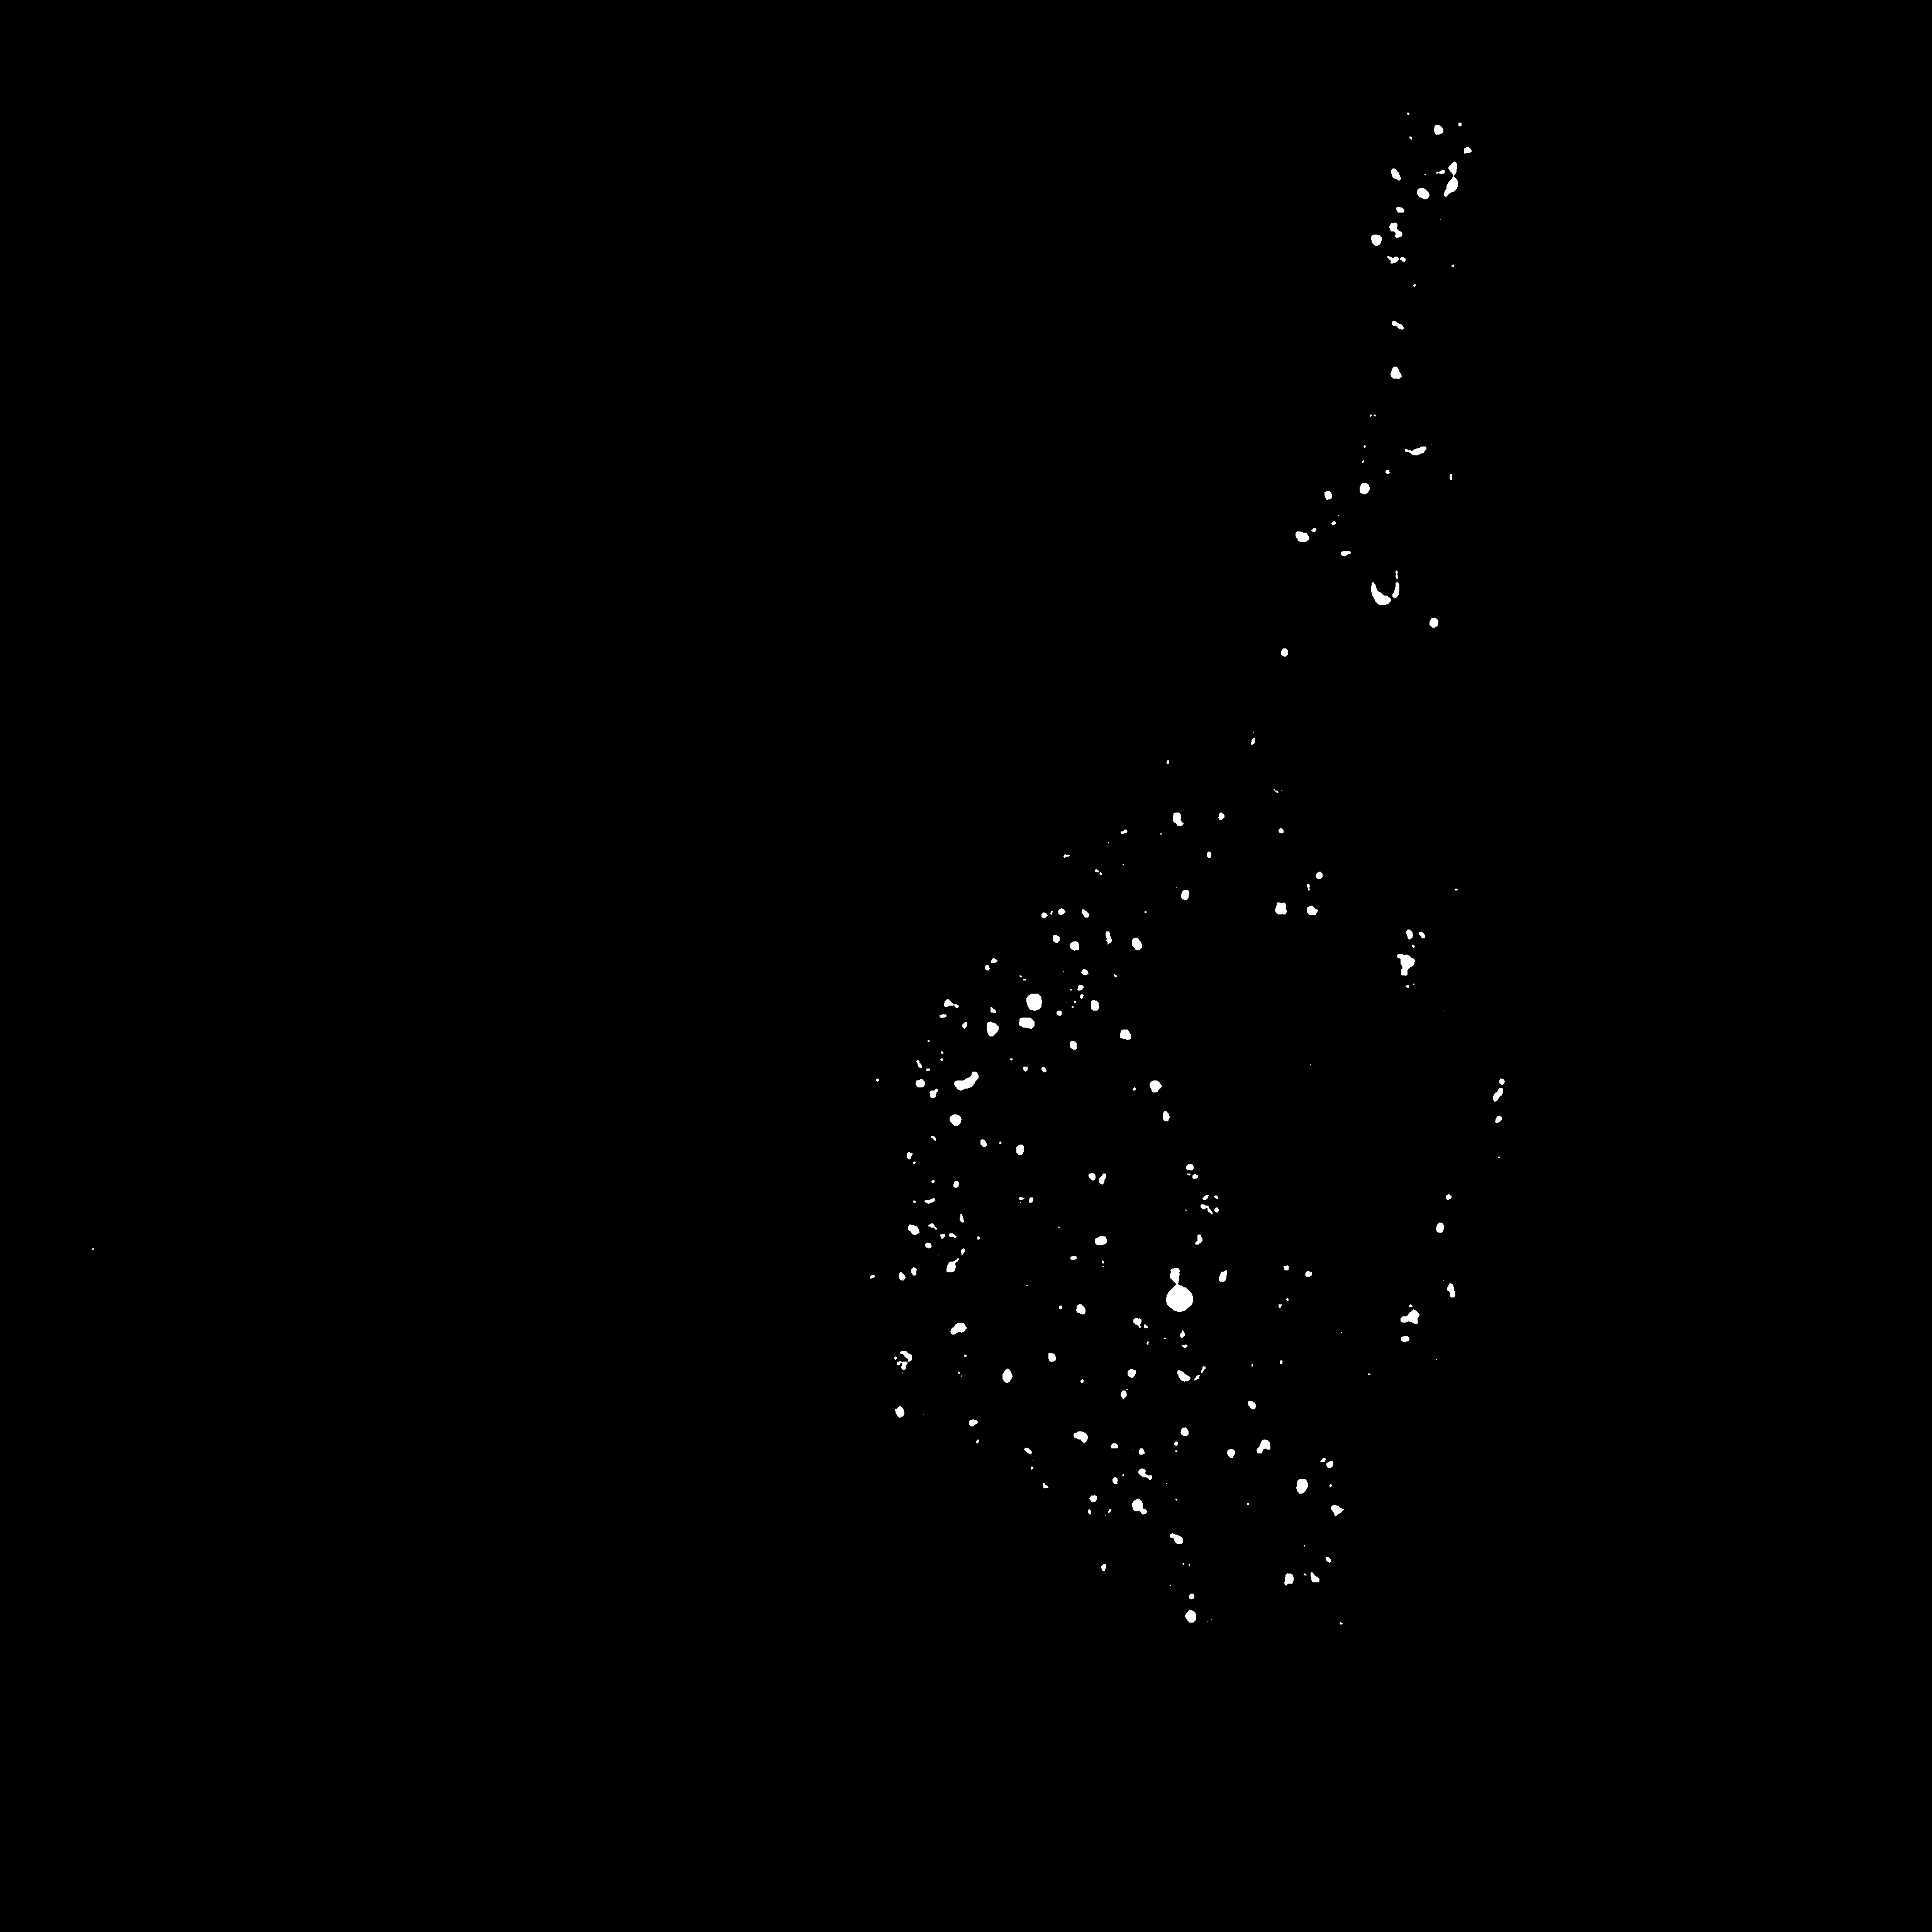
\includegraphics[width=0.49\linewidth]{figs/ch2figs/N2Con_3C=0T=0_noclahe_otsu.png}}
    \subcaptionbox{Binarised image after the Otsu threshold has been to image \subref{subfig:middleslice_clahe})\label{subfig:clahe_otsu_applied}}{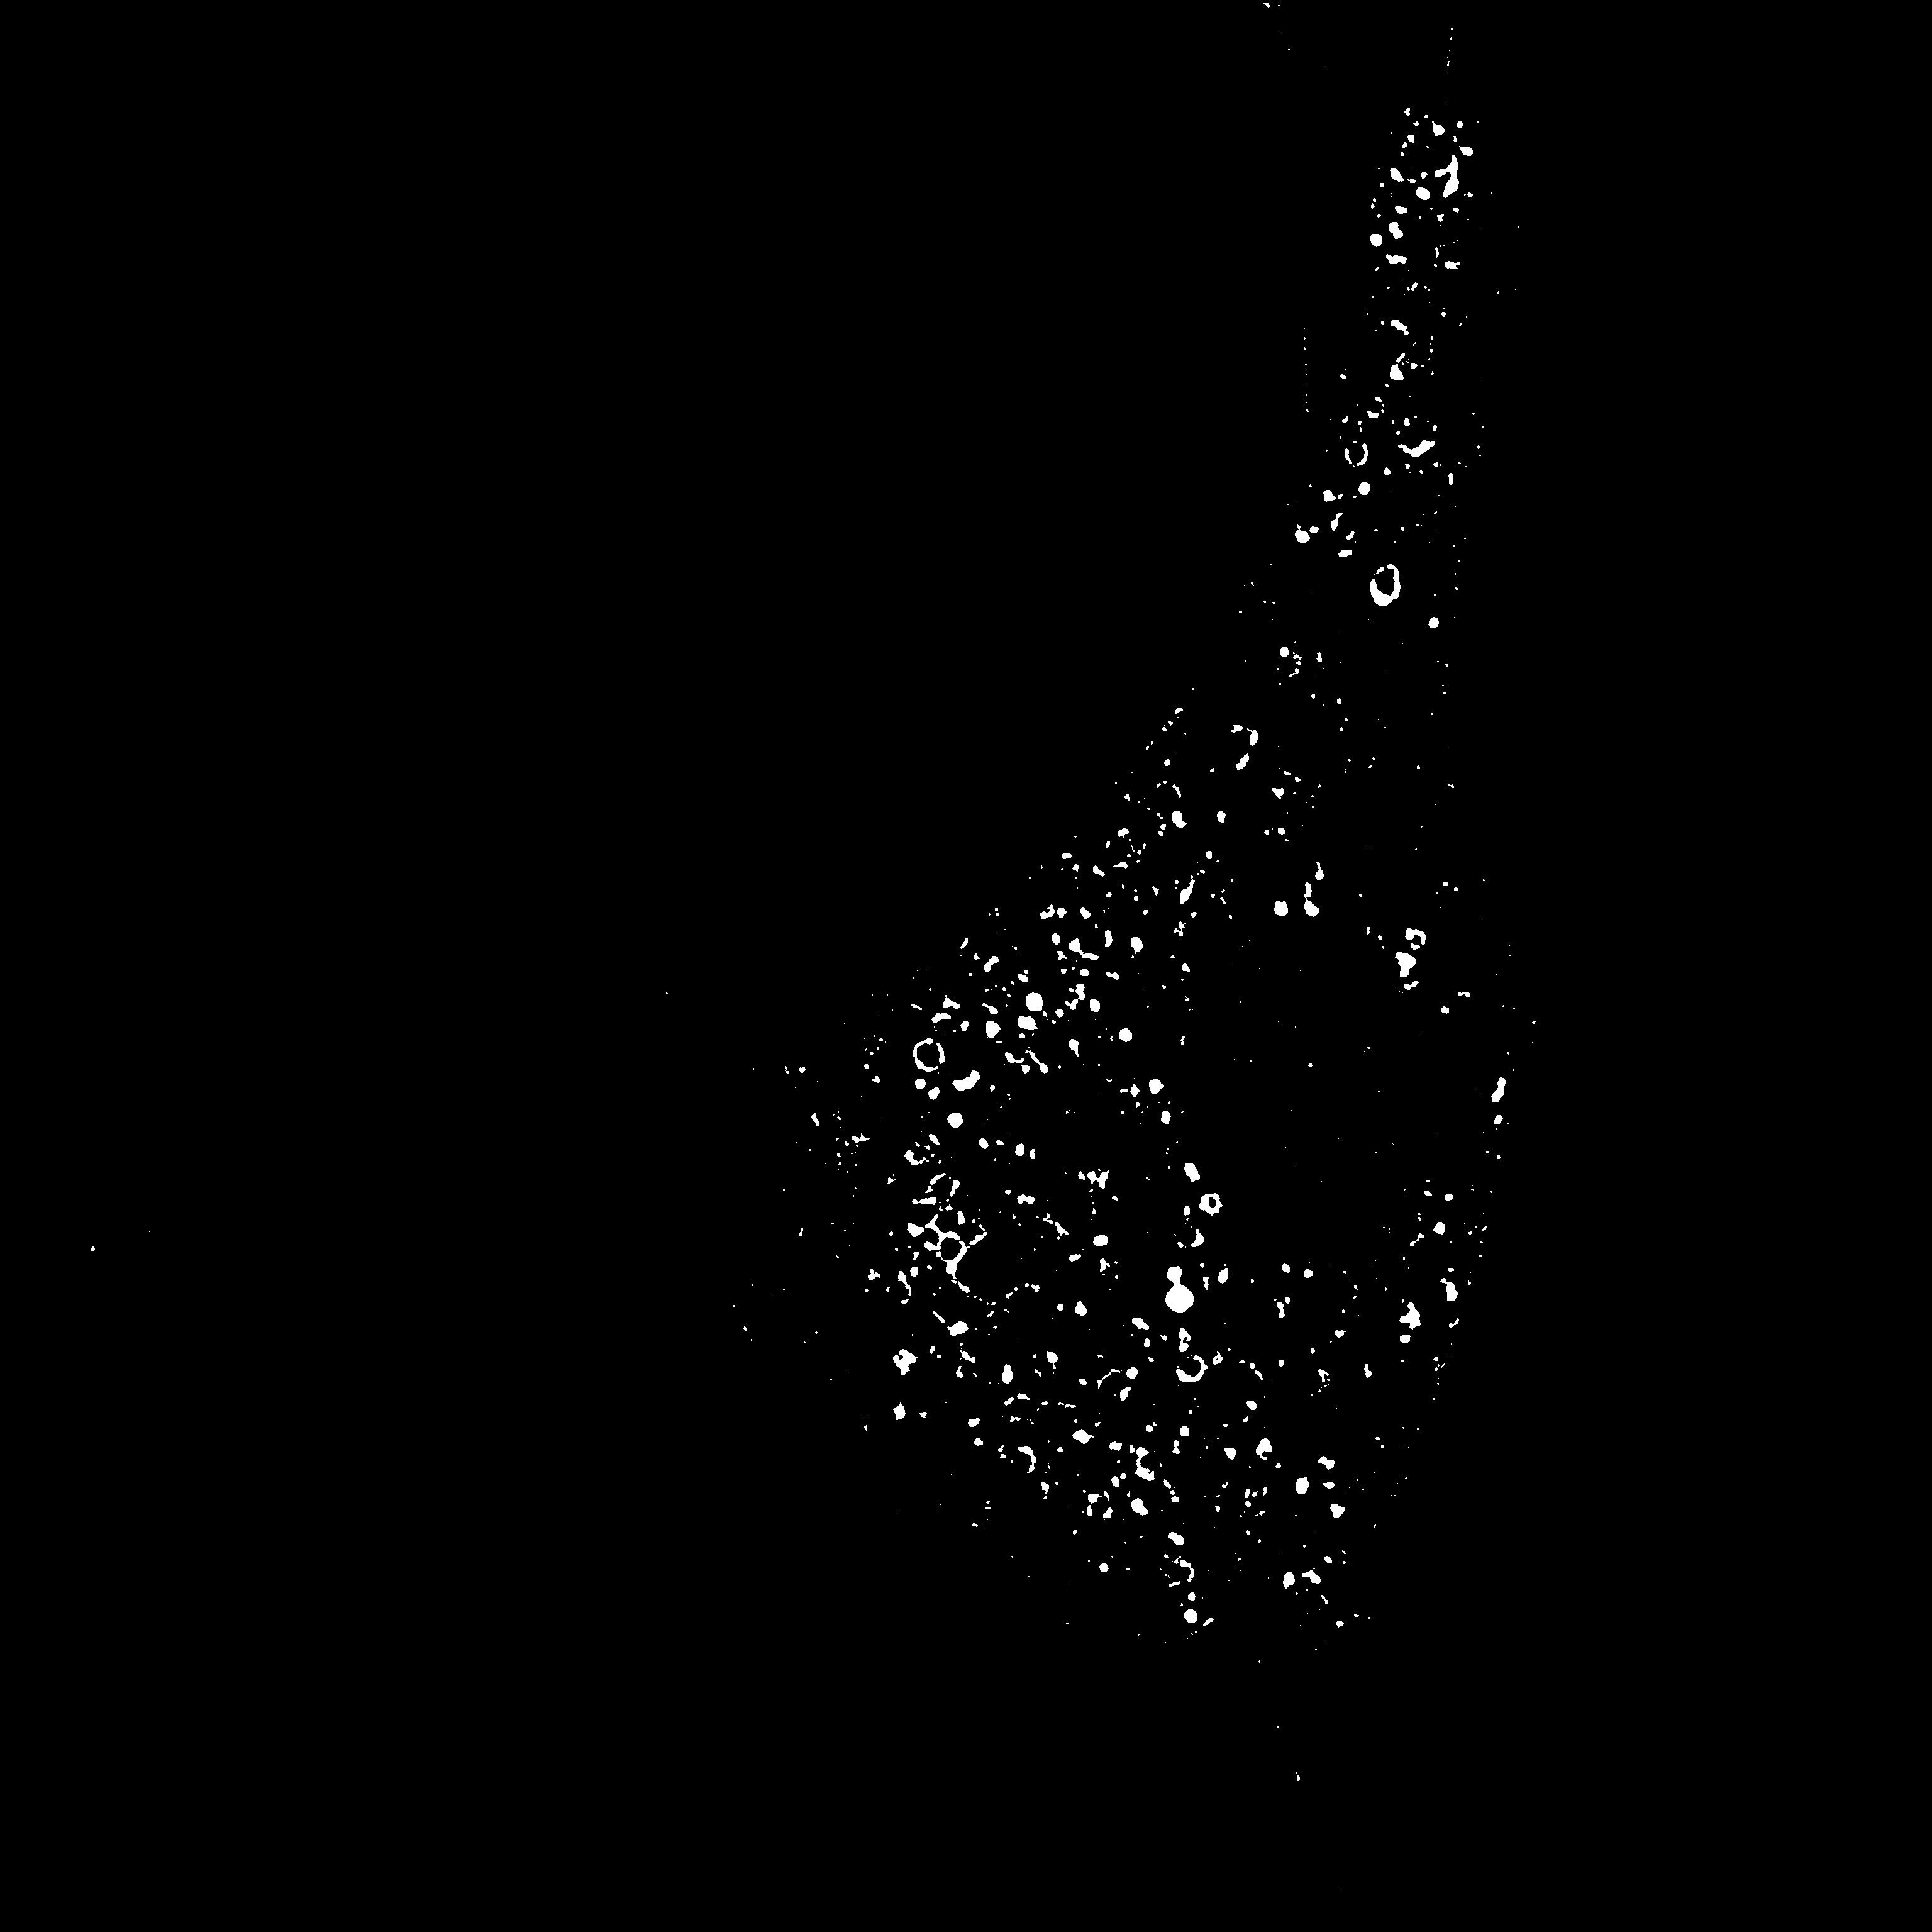
\includegraphics[width=0.49\linewidth]{figs/ch2figs/N2Con_3C=0T=0_clahe_otsu.png}}
    
    \caption[Visual showcase of the effect of contrast enhancement on image thresholding]{The impact of contrast enhancement on the image analysis process is presented regarding the automated thresholding between foreground and background structures. The specimen image is shown in (\subref{subfig:middleslice_noclahe}) which has had background subtraction applied and CLAHE has been applied to this image to restore contrast as shown in (\subref{subfig:middleslice_clahe}). The impact of this on global thresholding (Otsu) is shown in (\subref{subfig:otsu_before_clahe}) which is Otsu applied before CLAHE and (\subref{subfig:clahe_otsu_applied}) is the result of Otsu after CLAHE has been applied.}
\end{figure}
\par
\textcolor{red}{For the background subtraction, I have been struggling to find images to which I can apply background subtraction myself (that actually have uneven illumination). Do you think it is fine if I use this image from scikit-image? \textit{https://scikit-image.org/docs/stable/\_images/\\sphx\_glr\_plot\_rolling\_ball\_001.png}}
\subsubsection{Thresholding}\label{subsec:thresholding}
Thresholding is a method by which pixels are assigned a label dependent on the pixel value in relation to a threshold value (lesser or greater than). In a pre-processing context, this is typically applied to differentiate between foreground and background pixels. This functions under the assumption that objects of interest in the image will be composed of pixels with a value greater than the threshold thus all objects of interest will be assigned to the foreground. Background pixels on the other hand are artefacts, noise or objects not of interest (appearing due to autofluorescence, out-of-focus fluorescence, or bleed-through). After threshold application, only the foreground pixels, those belonging to objects of interest, will be preserved.\par Outside of pre-processing threshold methods technically fall under image segmentation which is a body of techniques that assign labels to pixels based on some criteria. Image segmentation has a myriad of methods depending on the field of application (microscopy, morphological analysis, object detection, etc.) where the number of labels is determined by the number of groups that an object, described by pixels, can belong to. This application is relative to pre-processing thus the focus is on thresholding images to get binary classifications (foreground or background).\par With the binary classification of images to separate pixels composing objects of interest from `other' pixels (where `other' refers to noise, artefacts and inconsistent background illumination) a single threshold value is required to classify each pixel. This classifying behaviour is consistent across all threshold methods but the determination of the threshold value is what changes between methods. There are two groups of threshold methods which are global thresholding and local thresholding~\cite{segmentation_book} with the former determining a threshold using and applying it across the entire image while the latter determines and applies the thresholds across localised regions of the image.
\paragraph{Global thresholding}
Global methods, like \textit{Otsu thresholding}~\cite{Otsu1979ATS}, determine the threshold value using the image histogram by selecting an intensity value separating the histogram values into two groups. In ideal situations with a distinct separation between the grey-level intensities of the background and foreground will be characterized in the histogram with two peaks where the clusters centred around each peak correspond to the pixels for the foreground (higher intensity) and background (lower intensity) respectively~\cite[p.163]{segmentation_book}. An example of this can be seen in Figure \ref{fig:histogram_appearances} where the different potential histogram shapes are displayed.
\begin{figure}
    \centering
    \subcaptionbox{Bimodal histogram}{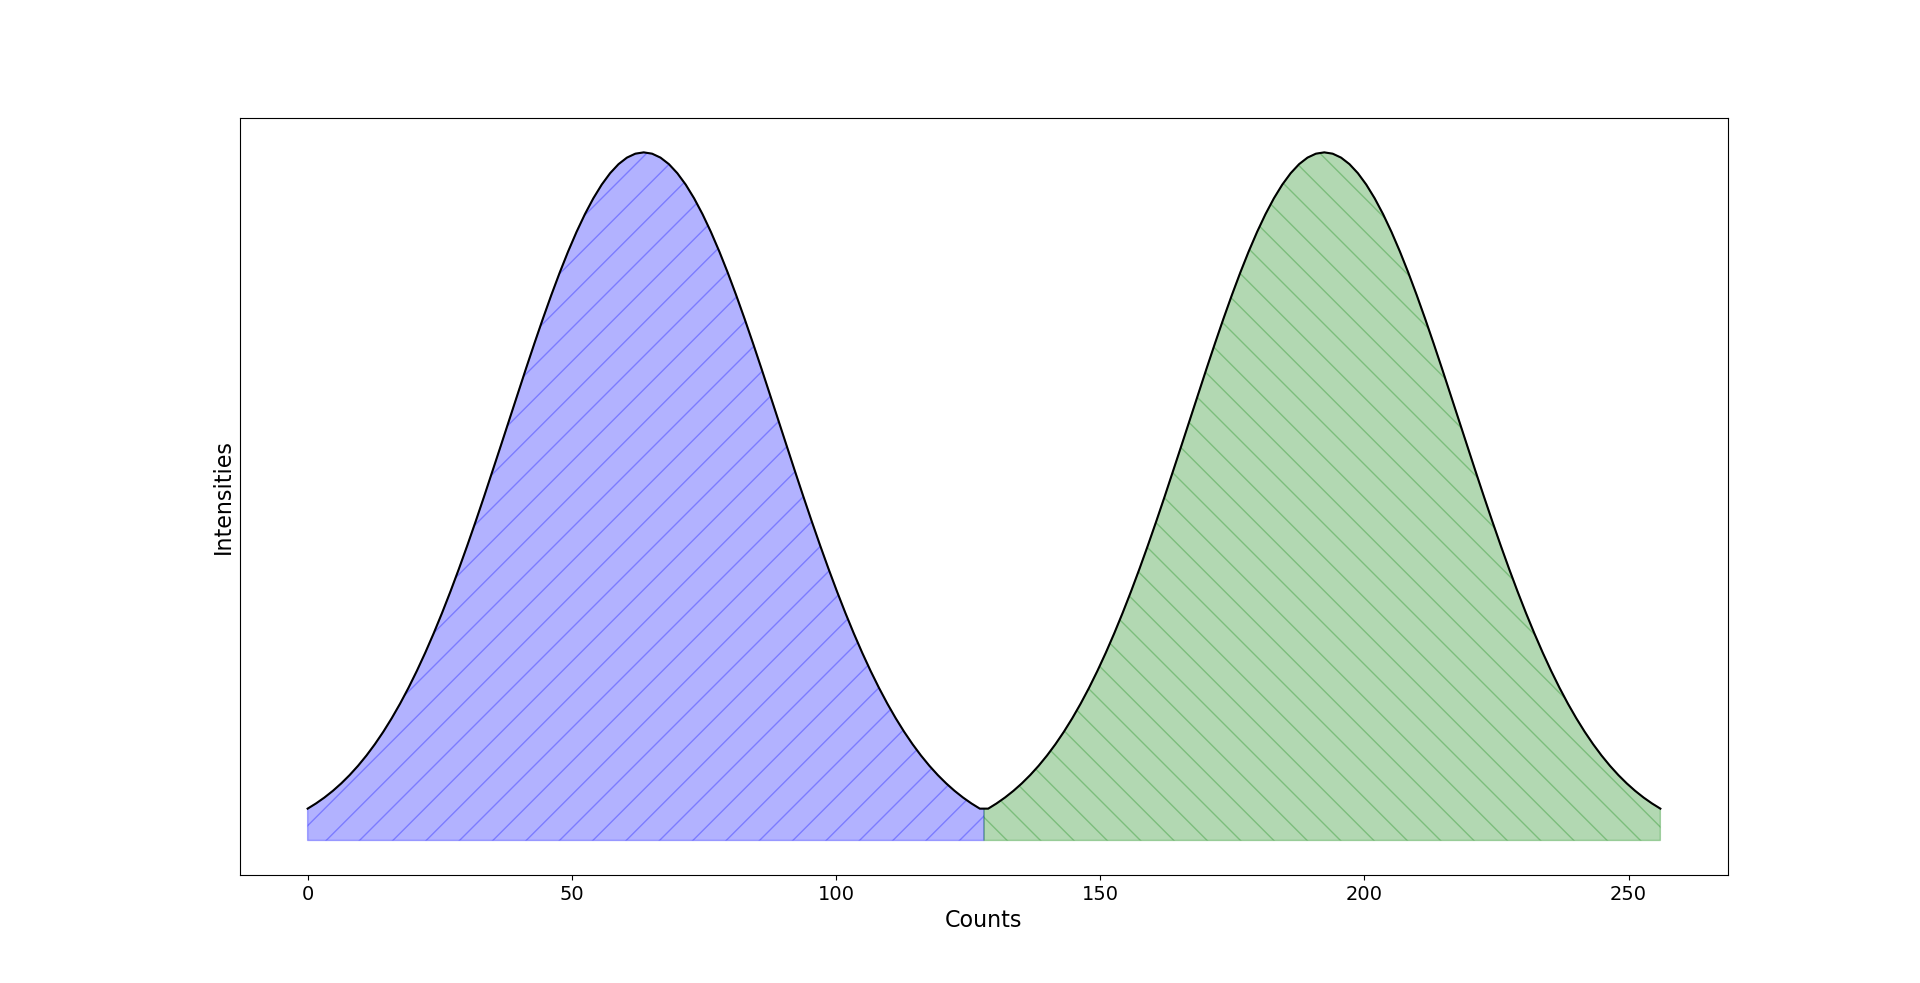
\includegraphics[width=0.32\linewidth]{figs/ch2figs/Bimodal.png}}
    \subcaptionbox{Unimodal histogram}{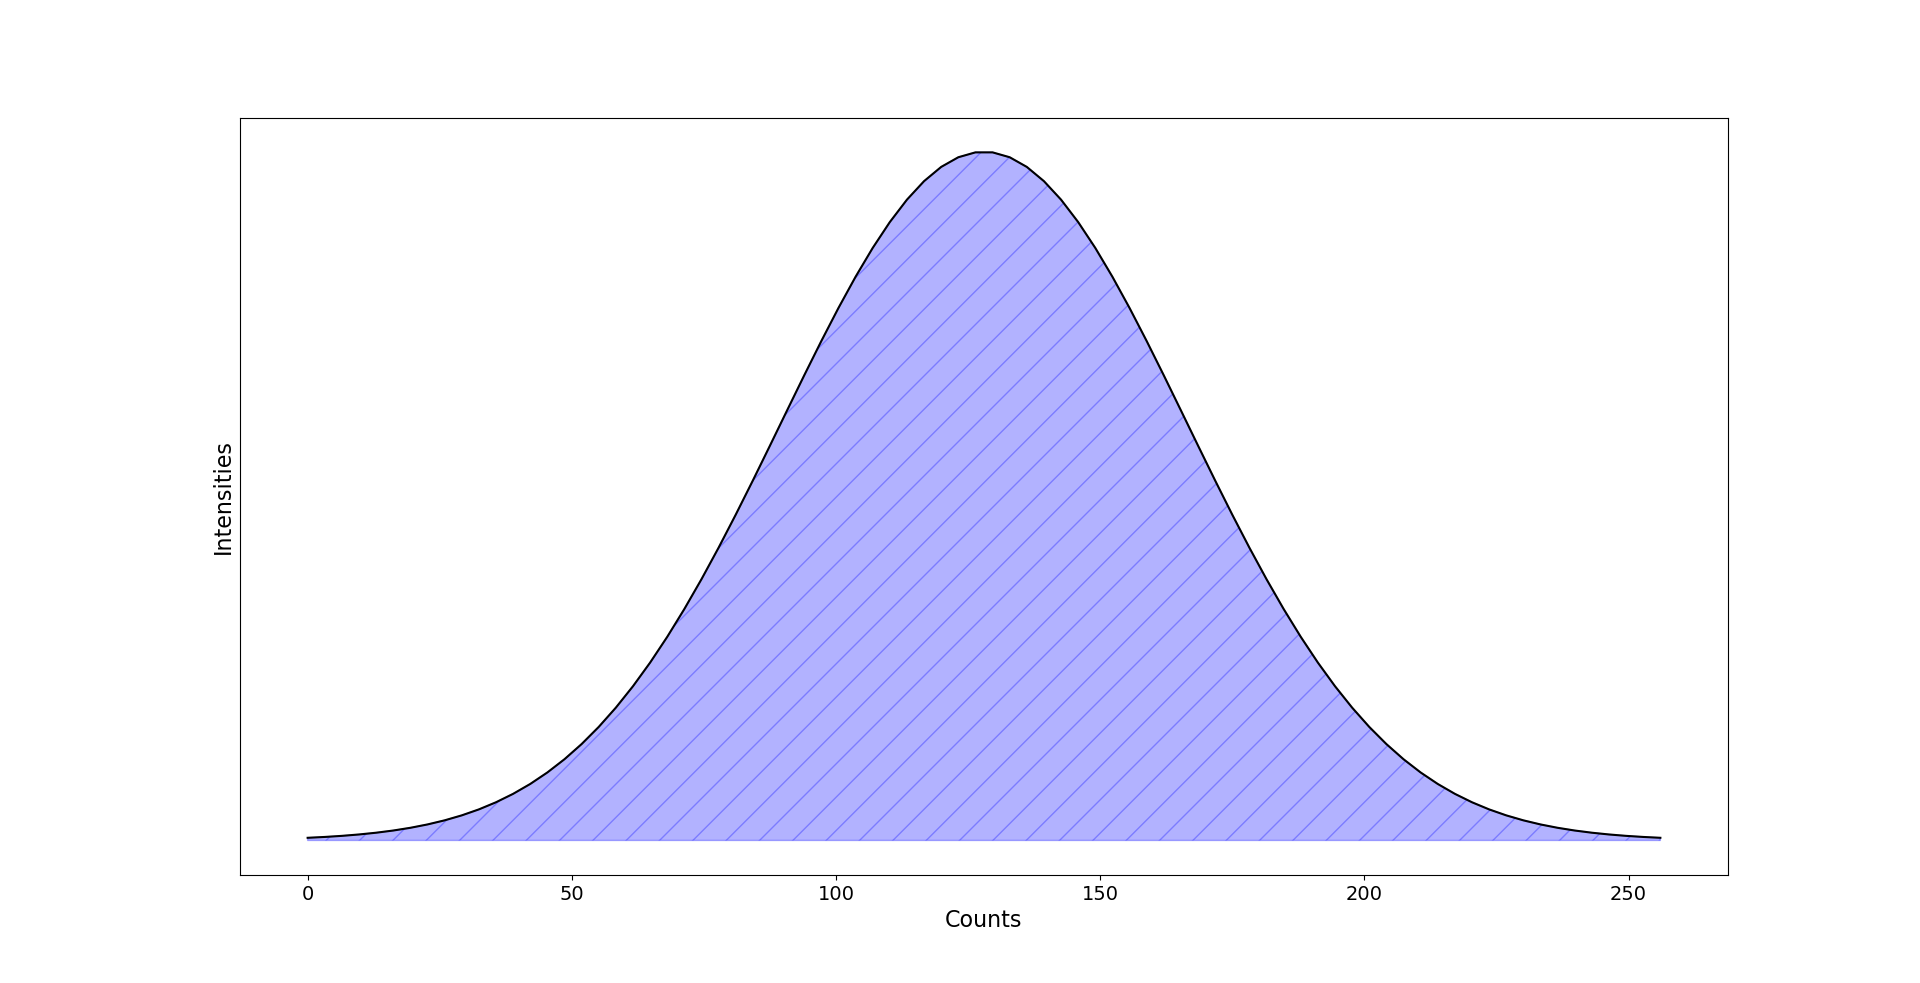
\includegraphics[width=0.32\linewidth]{figs/ch2figs/Unimodal.png}}
    \subcaptionbox{Dominant background histogram}{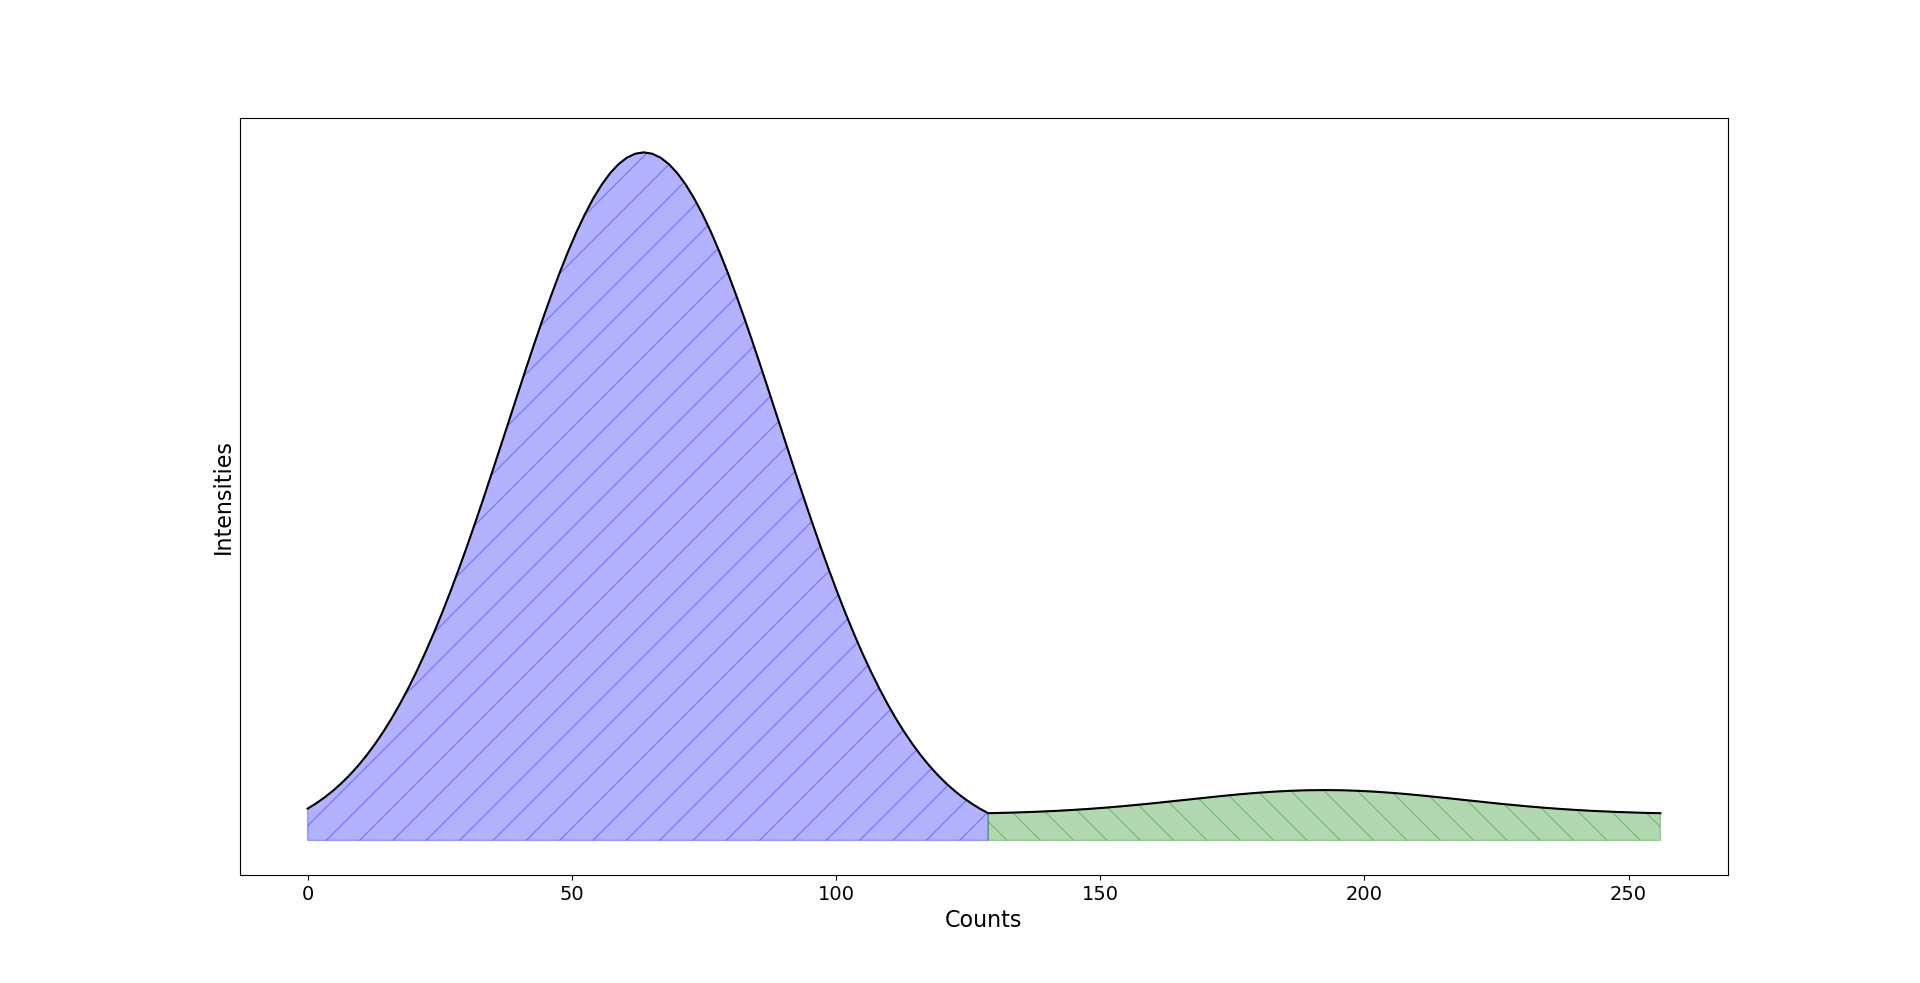
\includegraphics[width=0.32\linewidth]{figs/ch2figs/dominant_background.png}}
    \caption[Three common histogram modalities]{Three common histogram modalities with each mode being visually labelled with different colours and hatching (blue vs green and hatching direction).}
    \label{fig:histogram_appearances}
\end{figure}
When there are distinctly two peaking crests with limited overlaps of their bodies in the trough (as indicated in Figure \ref{fig:histogram_appearances}) then the histogram is referred to as bimodal. The further the histogram shape diverges from bimodal the less effective global thresholding becomes as the threshold value to separate the foreground and background becomes less clear. When this threshold value becomes uncertain then there is a greater risk of false classification of either background or foreground pixels. The greater the quantity of noise and artefacts, particularly of intensities close to the foreground pixel intensities, the worse global thresholds perform.
\paragraph{Local thresholding}
These threshold methods address this sensitivity to the histogram shape deviating from bimodal (which can be caused by noise, artefacts, and uneven illumination among others) by evaluating the image itself. This is achieved by performing calculations within sub-regions of the image and applying the threshold value derived by these calculations to this sub-region itself~\cite[p. 72]{bioimage_book}. A notable local thresholding method is \textit{Adaptive thresholding}~\cite[p.162]{segmentation_book} which calculates some threshold value by applying an operation across the pixel values within a square neighbourhood of shape $n\times n$ where $n$ specifies the size of the neighbourhood. The neighbourhood is of an odd size so that the centre of the neighbourhood can be on the currently thresholded pixel. The operation applied to the neighbourhood to calculate said threshold, in \textit{adaptive thresholding}~\cite{adaptive_thresh_plugin}, typically being that of the mean or the weighted (Gaussian) mean of the neighbourhood and potentially further tuning of the threshold strictness by the subtraction of some constant.\par Some adaptive thresholding approaches employ the variance or standard deviation of pixel neighbourhoods as a thresholding criterion but there is no definitive adaptive thresholding approach as each was developed under a specific use case. Of note is that Adaptive thresholding is sensitive to neighbourhood size as the threshold is determined by the local mean and/or variance. The threshold employed is basically that the greater the magnitude of the central neighbourhood pixel, currently being thresholded, than the surrounding pixels then the higher the likelihood it will be preserved yet if the central pixel magnitude is quite similar to, or less than, the surroundings then it is removed. This functions well for high-contrast object edges and neighbourhoods large enough to capture both background and object pixels since neighbourhoods that are too small (fit entirely within the object with minimal background) can lead to loss of object pixels if the pixels composing the object are relatively homogeneous which is more typically inside object bodies with the greatest contrast typically being between objects and the background. Likewise, overly large neighbourhoods risk approximating the shortcomings of global thresholds when applied to this data which is that across the image the distribution of intensities between background and foreground is uneven. Adaptive thresholding methods have been implemented in \textit{OpenCV}~\cite{opencv_library} and \textit{imageJ}~\cite{adaptive_thresh_plugin} by the method described above. Examples of alternative methods have been presented by \textit{A New Local Adaptive Thresholding Technique in Binarization}~\cite{Singh2012ANL} and \textit{Adaptive Document Binarization}~\cite{adapt_sauvola}. 

\section{Further investigation into prominent deconvolution and image quality restoration methods}\label{sec:further_methods}
%Here we will discuss Richardson-Lucy for deconvolution, Otsu, Hysteresis, Triangle.
\subsection{Otsu thresholding}
Otsu Thresholding is an automatic thresholding method that determines a threshold to separate two classes of intensities within an image. These classes each occupy continuous ranges of grey levels (to be referred to as intensity values) across the image histogram such that the lower class will occupy a range of $1$ to $k$ and the upper class will occupy a range of $k+1$ to $L$ where $L$ is some maximum intensity for an image and $k$ is some determined intensity threshold for the image~\cite{Otsu1979ATS}. This threshold ($k$) is selected such that the variance within each class, the variance between both classes and the variance across the image is maximized. The Otsu threshold is not without shortcomings as a prominent issue is it requires the image to be bimodal (or at least approximately bimodal) such that it can determine an optimized threshold value.\par Images with multi-modal histograms or images with noise that disrupts the desired modality of the image result in inaccurate threshold values. Over the years Otsu thresholding has been built upon in multiple papers to either improve the performance or to address multiple shortcomings. One such development resulted in an Otsu thresholding adaptation that can determine multiple thresholds for multi-modal images~\cite{MultiOtsu} but requires the expected number of classes to be provided before calculation. This is challenging in cases where the number of classes is unknown or the imaging conditions are such that the variance criteria are unrelated to legitimate classes creating confusion in the determined thresholds. In a theoretical and ideal example (illustrated in Figure \ref{fig:hypothetical_bimodal}), the threshold of a bimodal image will be within the valley between two peaks on the histogram where the between-class variance is maximal but in a case where the perceived modality is greater than one and a class expectation of two is provided, such that there are three peaks and two valleys on the image histogram, then the determined threshold may fall within either valley. In summary, Otsu thresholding performs best when the image histogram modality is two or more, the number of classes is known (the modality) and there are no aberrations across the histogram due to noise or other imaging conditions such that the modality of the image histogram is uncertain.

\begin{figure}
    \centering
    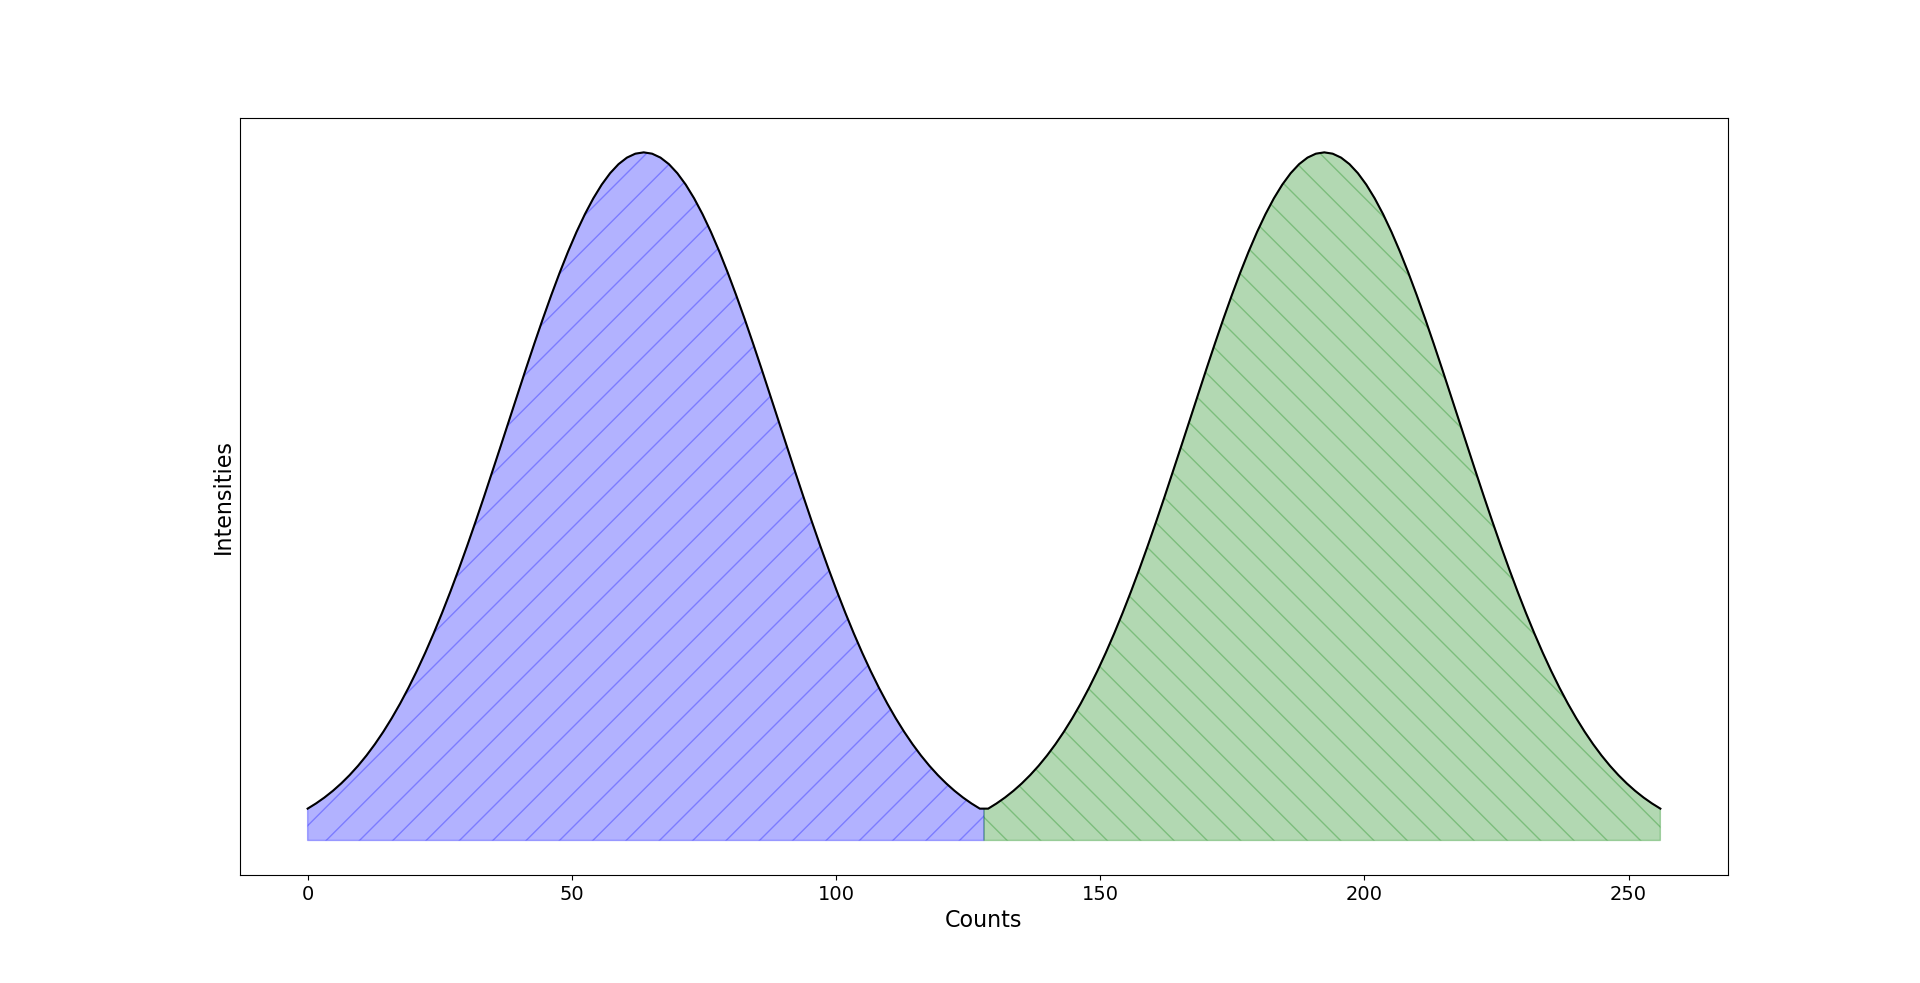
\includegraphics[width=\textwidth]{figs/ch2figs/Bimodal.png}
    \caption[A hypothetical and ideal bimodal distribution with the two modes separated in the centre]{A hypothetical and ideal bimodal distribution with the two modes separated in the centre. Each mode is defined by different colours and hatching styles with the separation point being at the ideal threshold value}
    \label{fig:hypothetical_bimodal}
\end{figure}
\par\textcolor{red}{Do you think the bimodal distribution (Fig. \ref{fig:hypothetical_bimodal}) is sufficient for the explanation of the behaviour of Otsu with an ideal modality?}

\subsection{Hysteresis thresholding} \label{sec:Hyst}
Hysteresis thresholding technique that utilizes two thresholds and evaluates pixels/voxels, for the remainder of this description pixels/voxels will be referred to as pixels, relative to their surrounding pixels for threshold application. The application of hysteresis thresholding is such that there are two provided thresholds where one can be designated as the high threshold $T_{Upper}$ and the other is to be designated $T_{Lower}$ where $T_{Upper} \geq T_{Lower}$ and $T_{Upper}, T_{Lower}\in\Re$. Across the image, any pixels greater than the $T_{Upper}$ than those pixels are immediately retained and any pixels below the $T_{Lower}$ are removed. For pixels that have a value between the $T_{Upper}$ and $T_{Lower}$, if it has a neighbouring pixel that has been retained (such as pixels with a value above $T_{Upper}$) then that pixel will also be retained. Thus structures containing pixels with continuous segments of pixels with values above the $T_{Lower}$ which connect to pixels with values above the $T_{Upper}$ are retained. It can be approximated that $T_{Upper}$ has significant control over the number of structures and that $T_{Lower}$ determines the possible volume of these structures where structures refer to continuous segments of pixels that represent some structure of interest in the image specimen/subject. A caveat of the Hysteresis threshold is the bias towards erroneously joining spatially close segments for values of $T_{Lower}$ that are too low thus indirectly affecting the structures count. One of the earliest descriptions of this method is in \textit{A Computational Approach to Edge Detection}~\cite{Hysteresis} where the method was applied to address streaking in images. where edge contours in images where streaking are \textit{``the breaking up of an edge contour caused by the operator output fluctuating above and below the threshold along the length of the contour''}~\cite[p. 689-690]{Hysteresis} which was described to be a problem more prevalent with single threshold value methods. An example of Hysteresis thresholding an the influence of erroneously selected threshold parameter values are shown in Figure \ref{fig:hyst_comparisons}.
%Add the 3D images with the sea level and mountains metaphor here so as to close off the understanding of what is considered a continuous contour
\begin{figure}
    \centering
    \subcaptionbox{The flattened maximum intensity projection (MIP) of the specimen image before Hysteresis\label{subfig:before_hyst}}{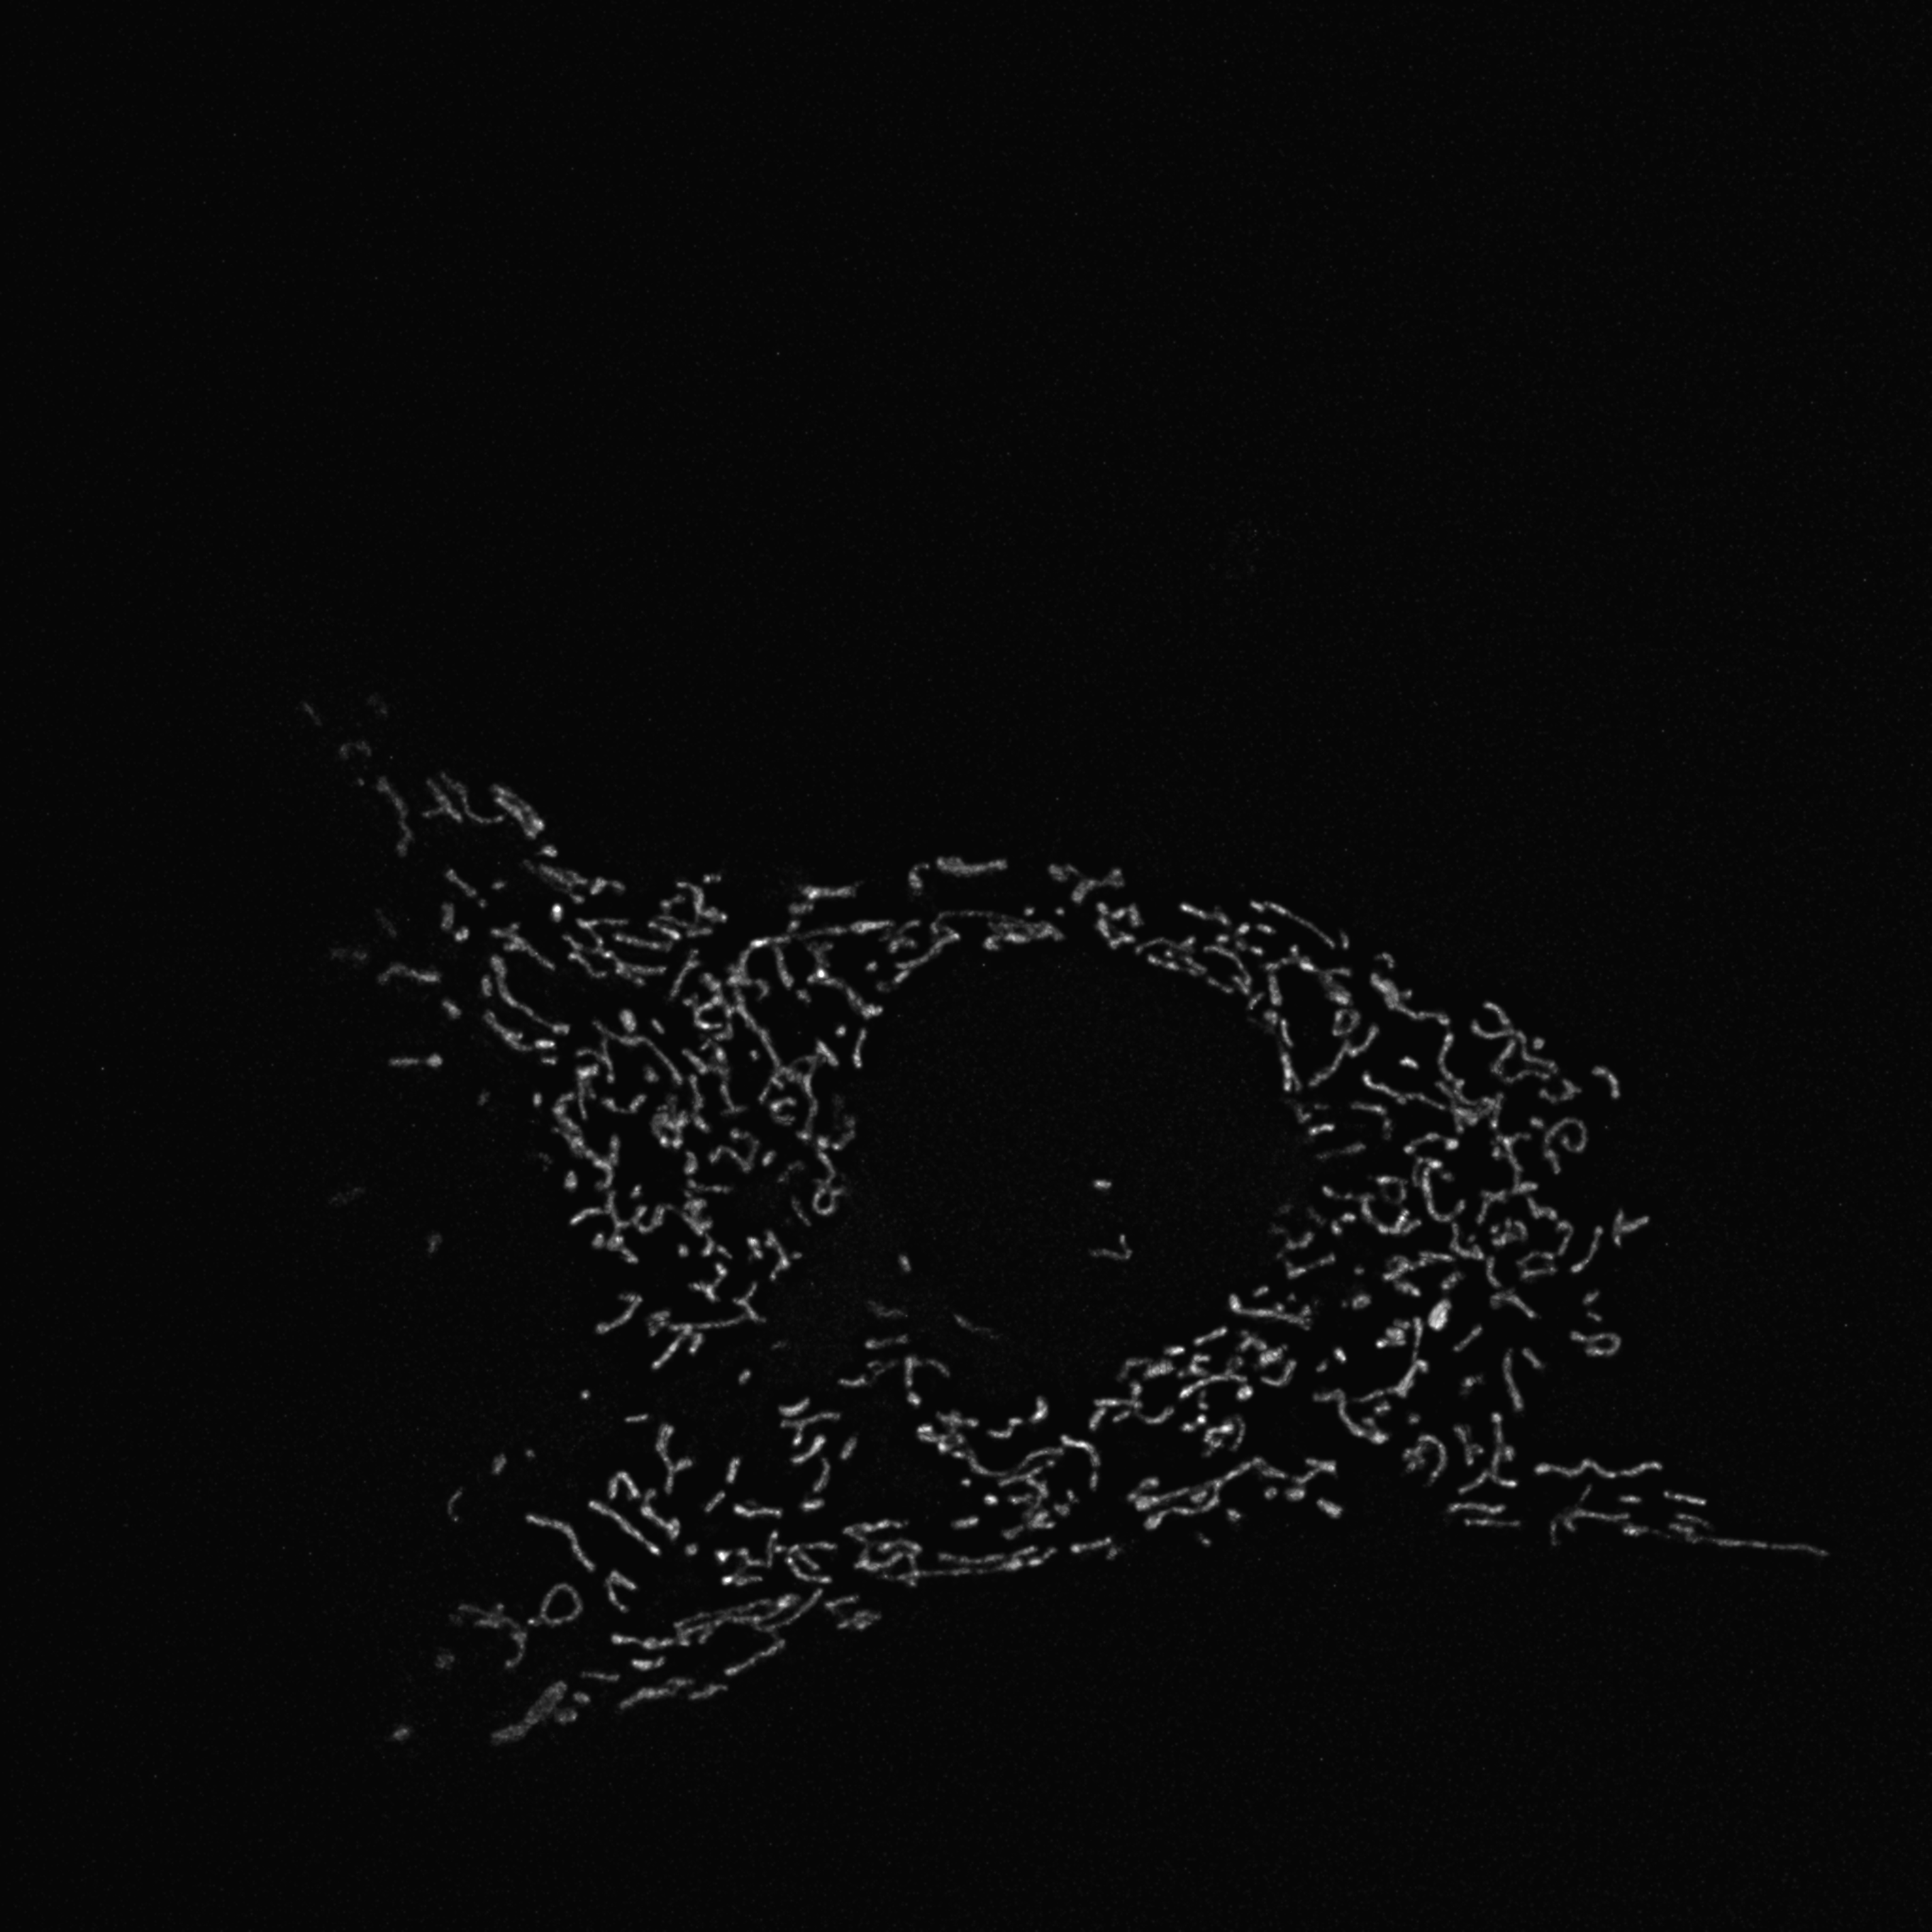
\includegraphics[width=0.49\textwidth]{figs/ch2figs/CCCP_1C=1T=0_normal.png}}
    \subcaptionbox{MIP with Hysteresis applied with good high and low threshold values\label{subfig:good_hyst}}{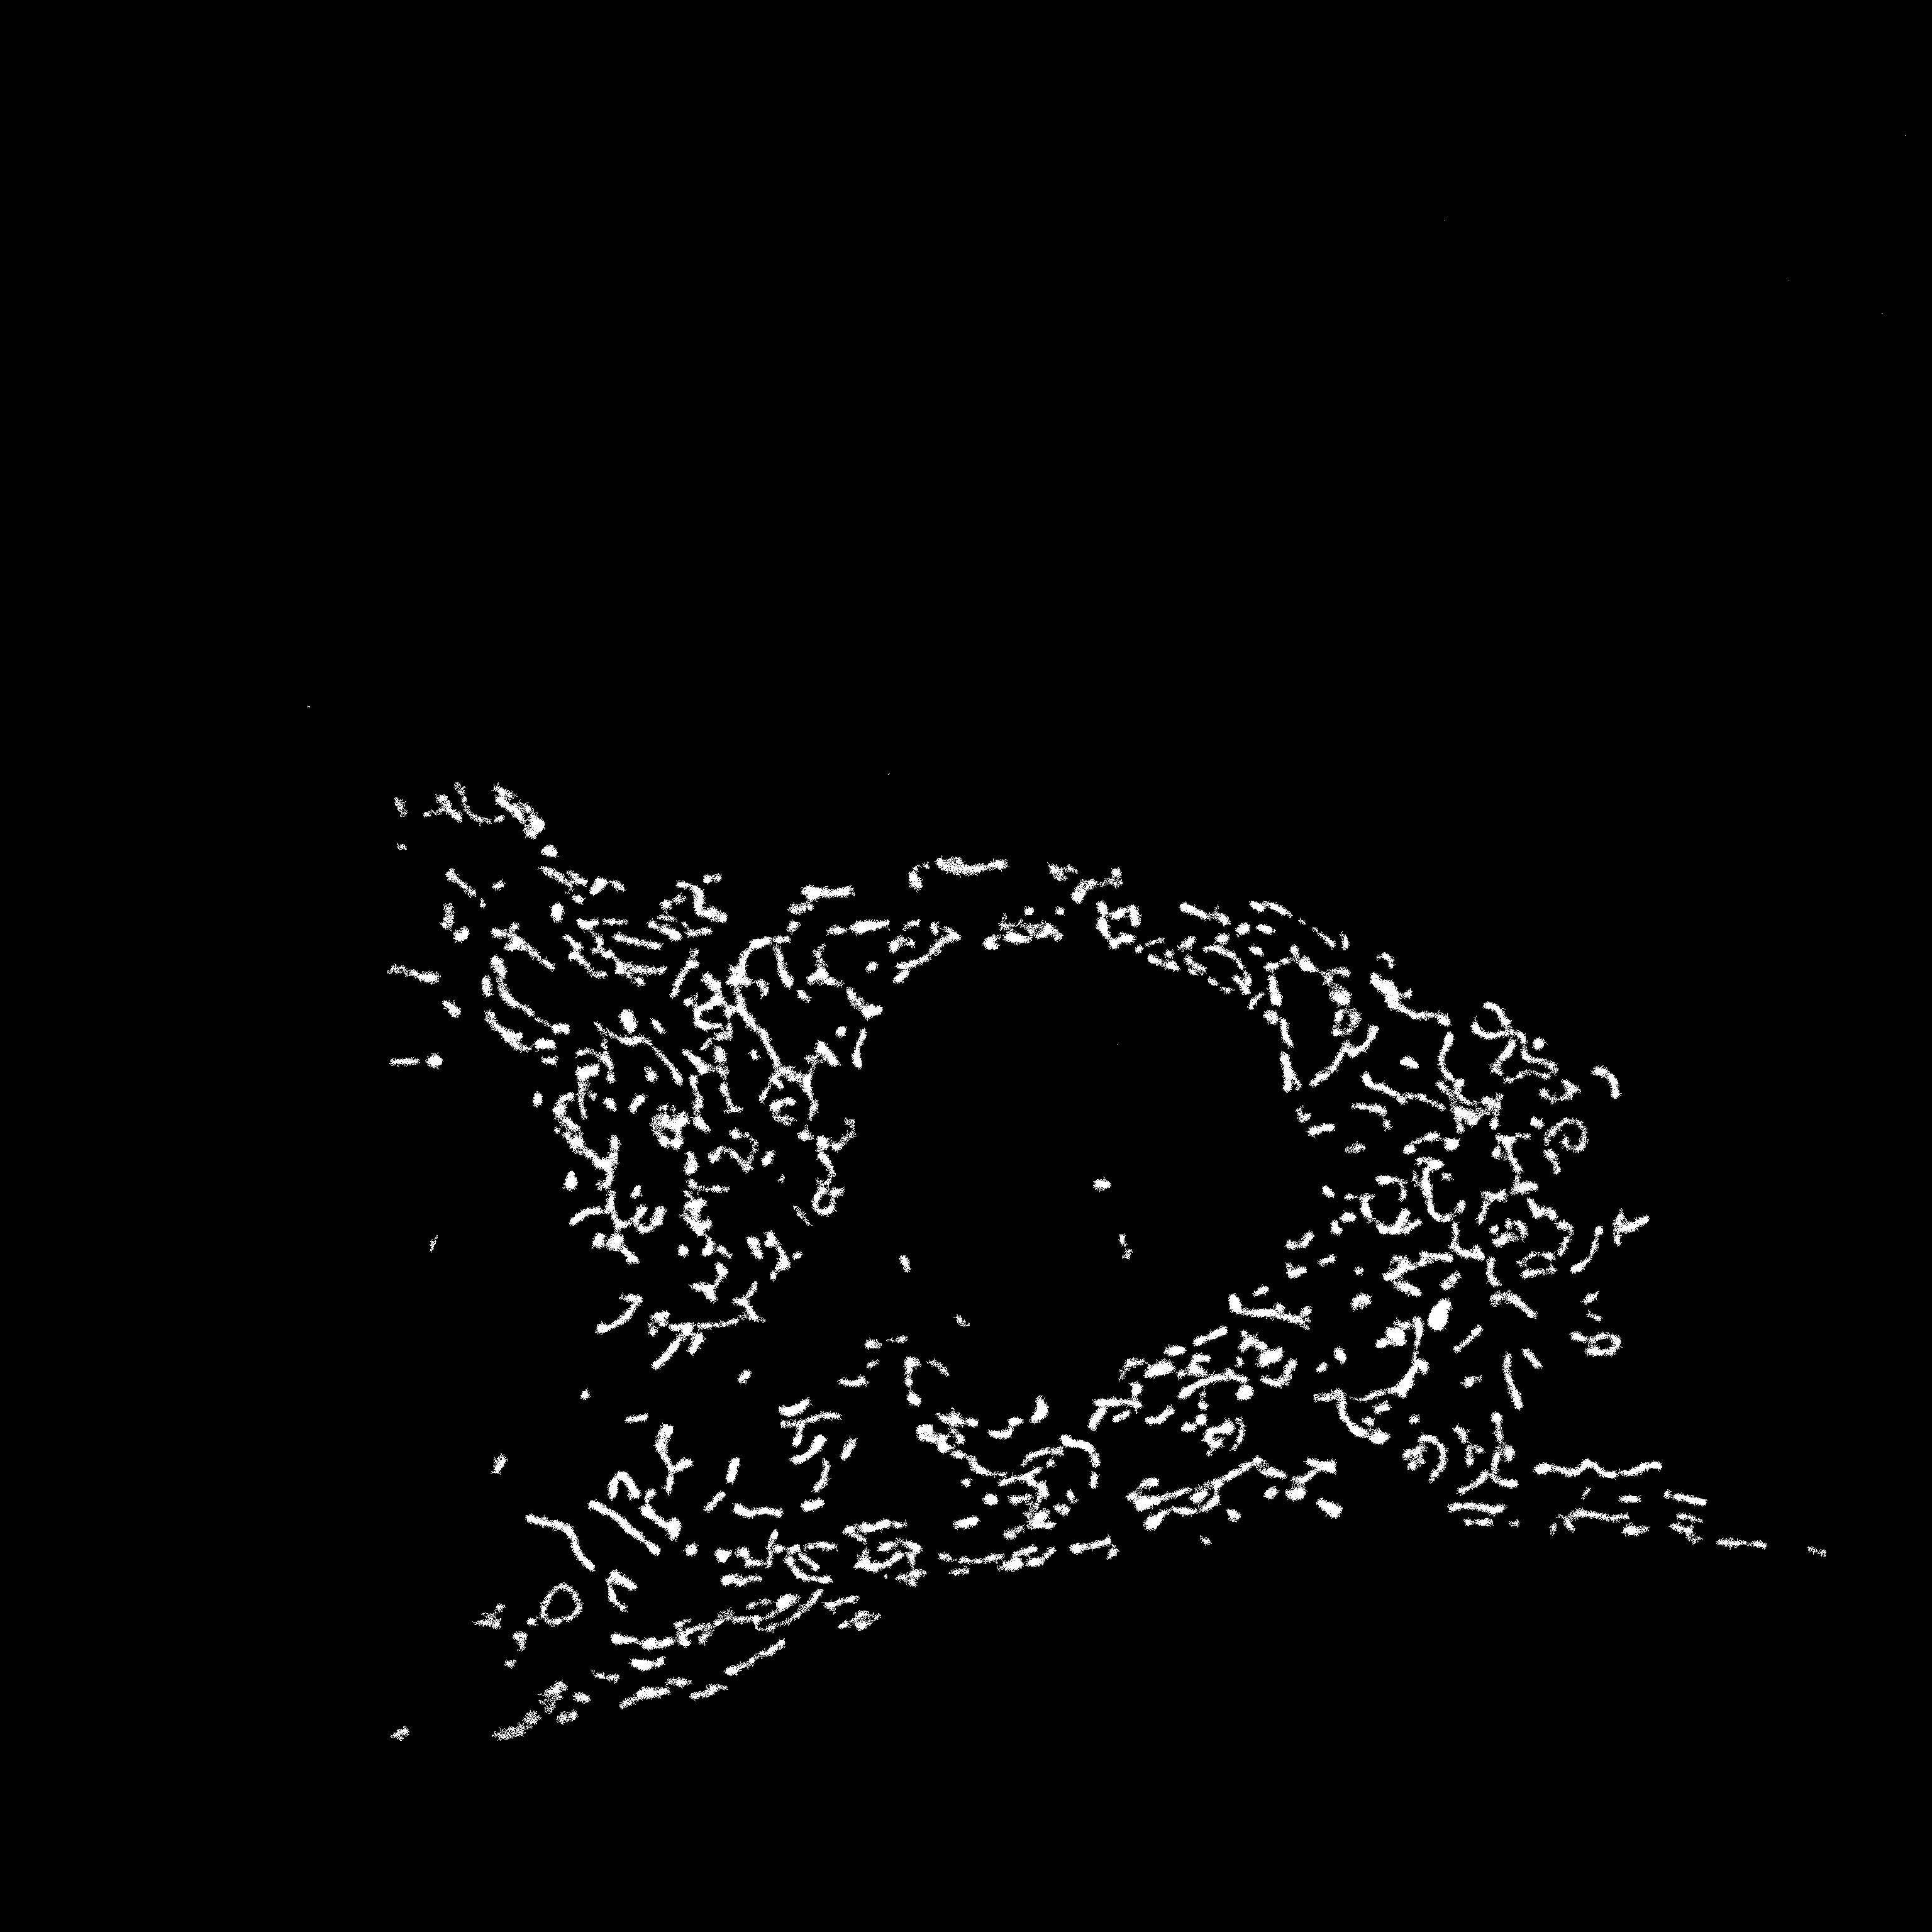
\includegraphics[width=0.49\textwidth]{figs/ch2figs/HystBin_CCCP_1C=1T=0_HystGood.png}}
    \subcaptionbox{MIP with Hysteresis applied with an overly strict (high) high threshold value retaining less individual structures\label{subfig:strict_hyst}}{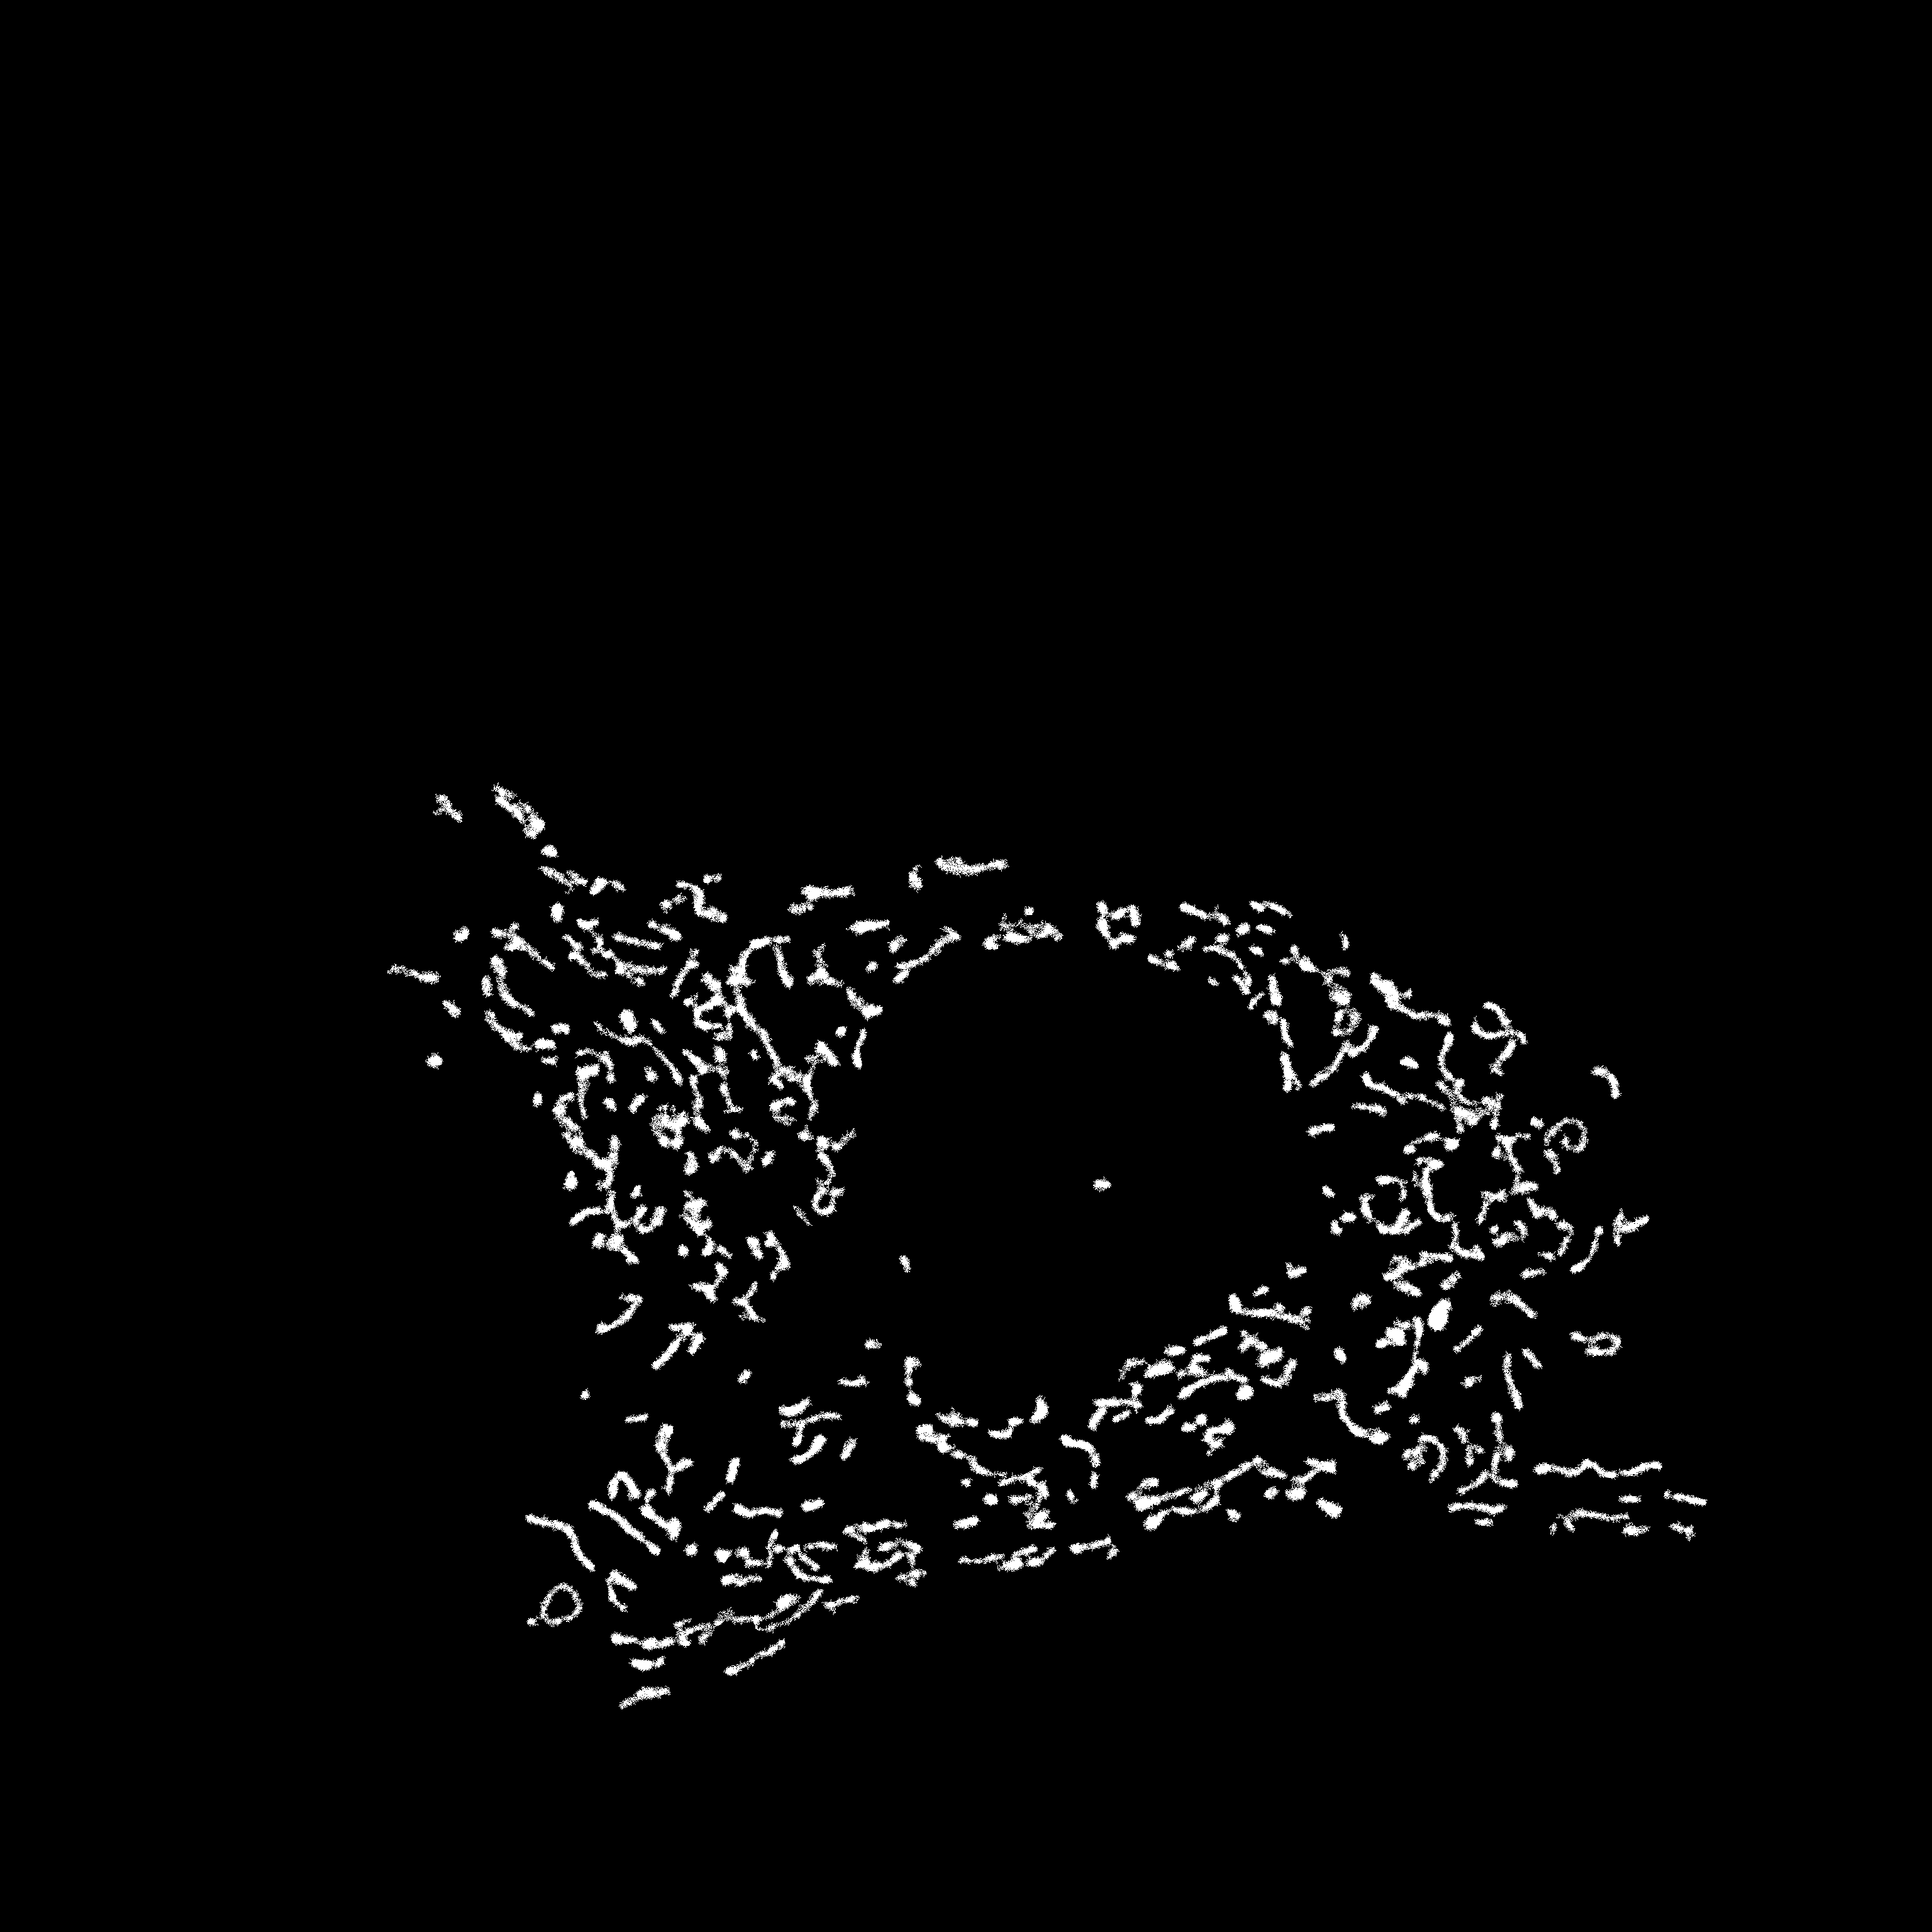
\includegraphics[width=0.49\textwidth]{figs/ch2figs/HystBin_CCCP_1C=1T=0_HighStrict.png}}
    \subcaptionbox{MIP with Hysteresis applied with an overly lax (low) low threshold retaining volume that is outside of the expected structures\label{subfig:lax_hyst}}{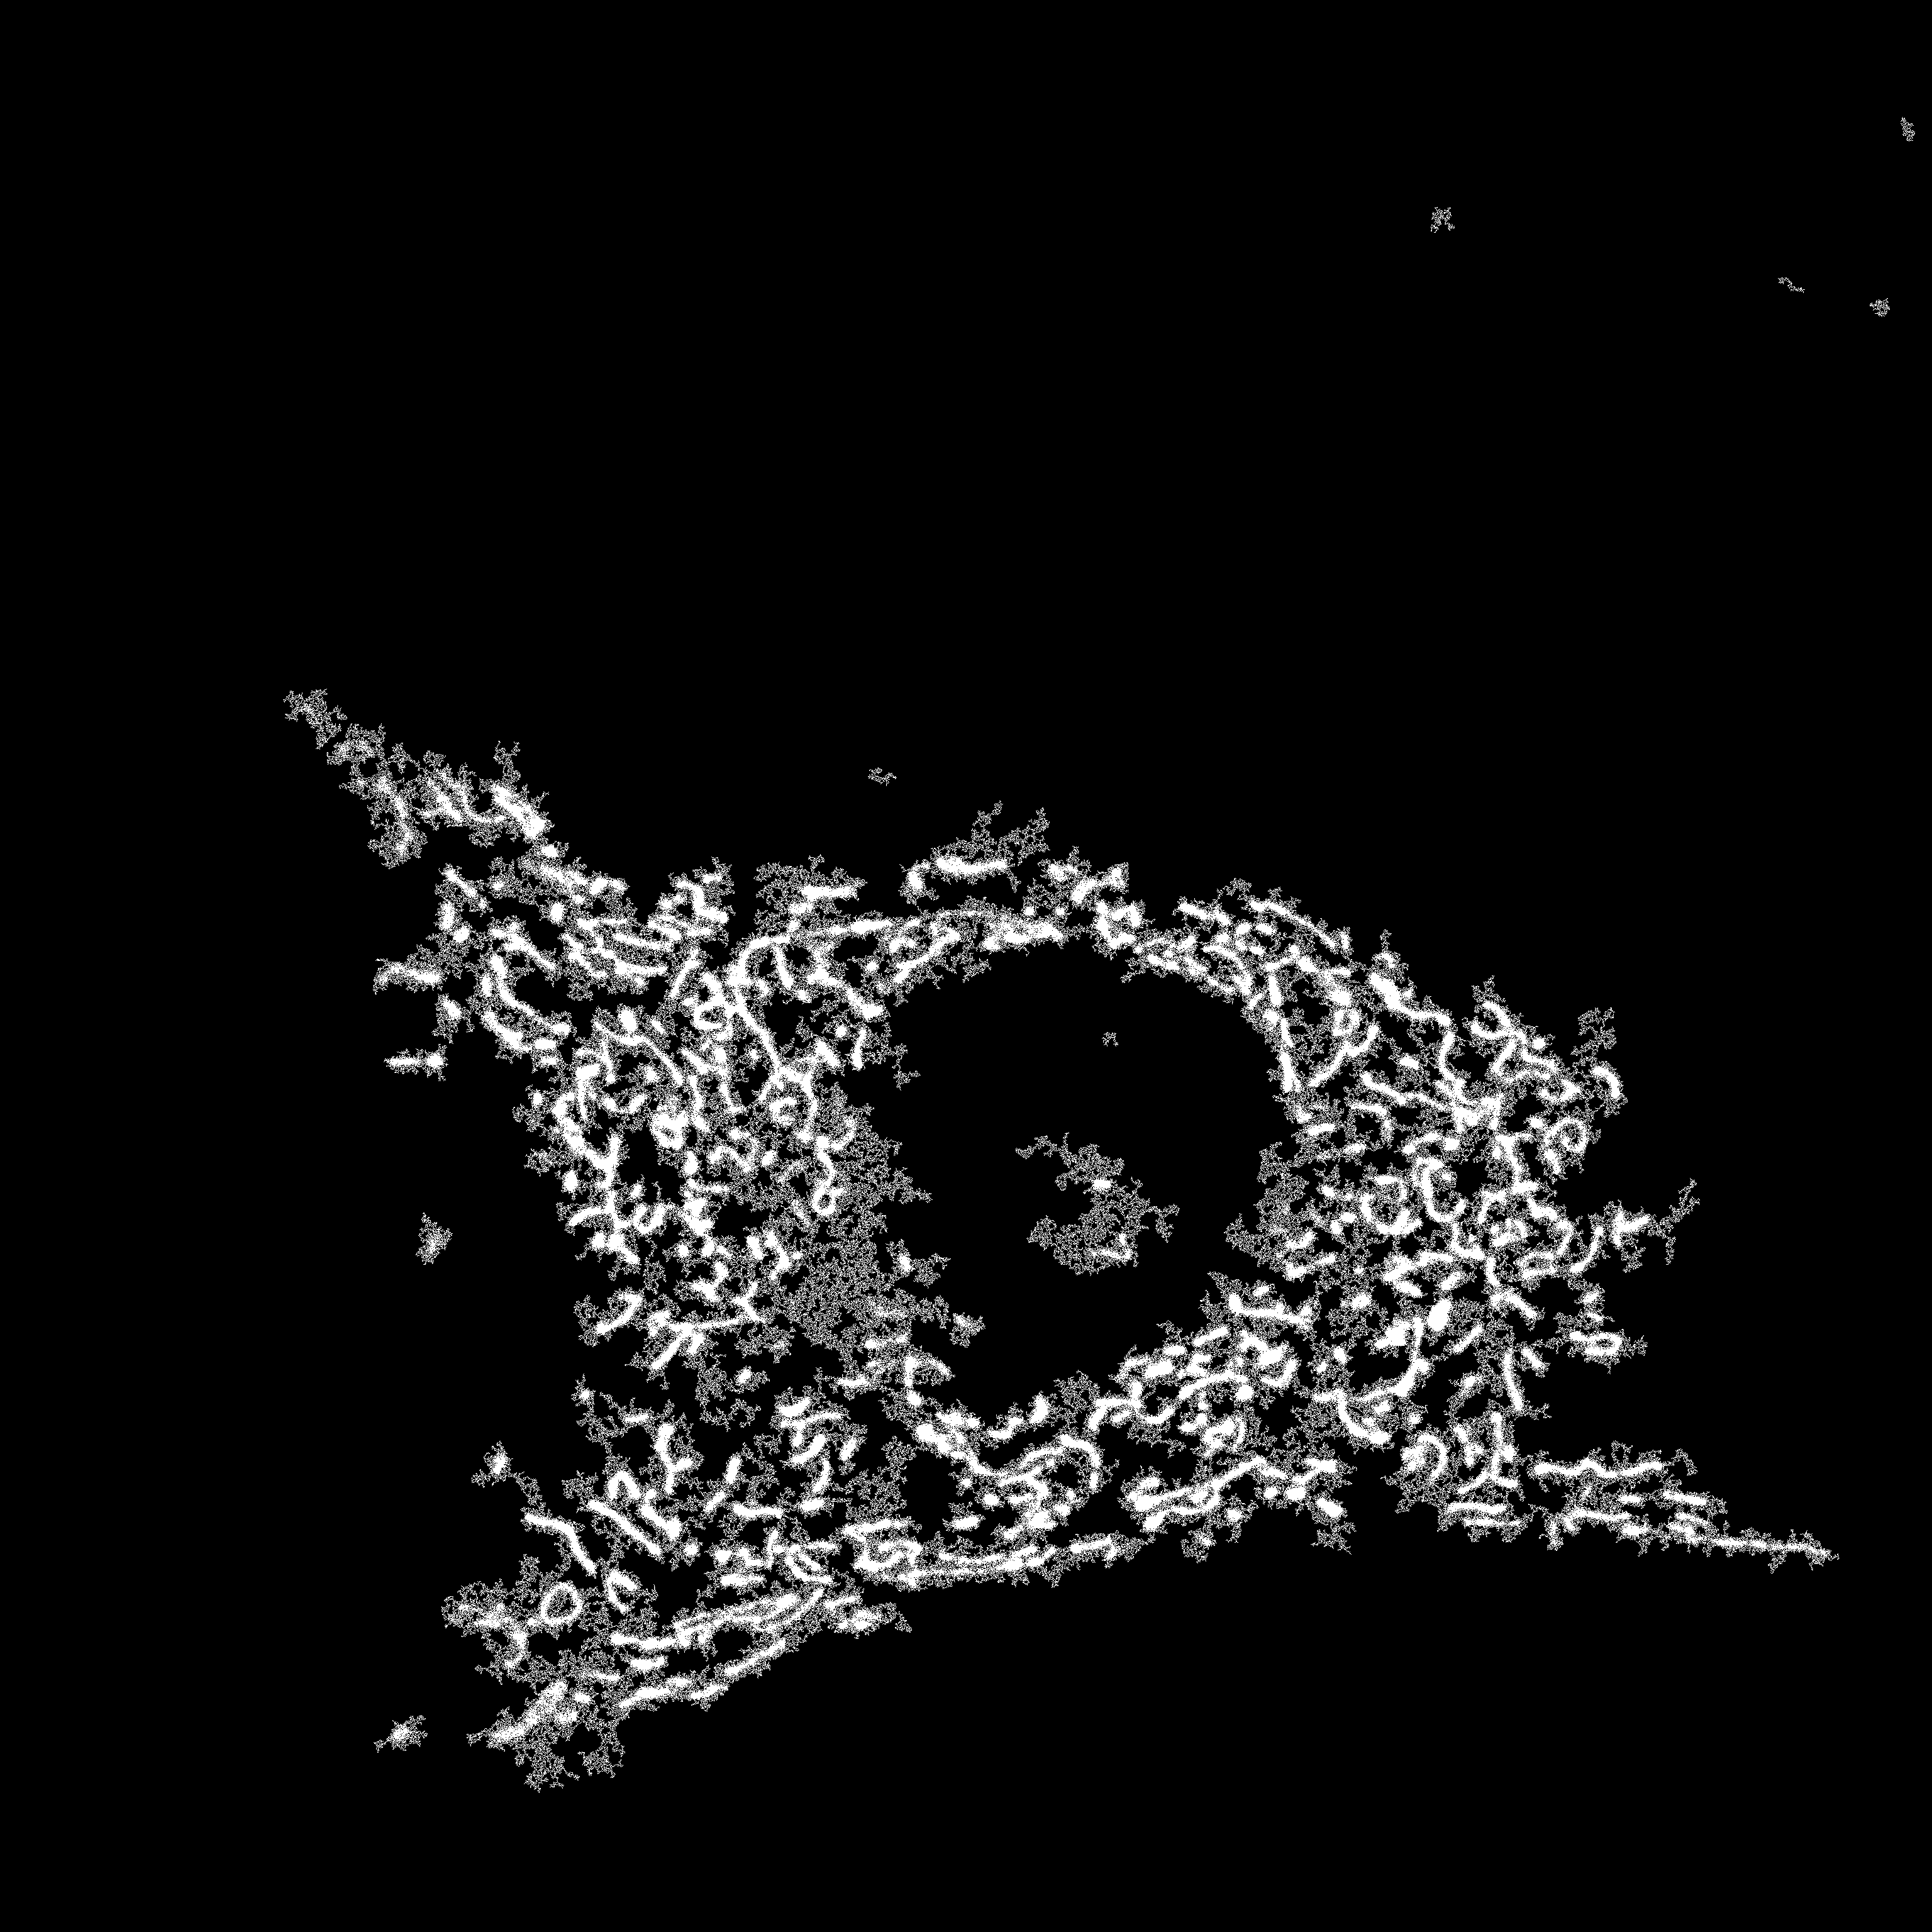
\includegraphics[width=0.49\textwidth]{figs/ch2figs/HystBin_CCCP_1C=1T=0_LowLax.png}}
    \caption[Comparison of the effect of Hysteresis threshold parameters]{Comparison of the effect of Hysteresis threshold parameters with the: \subref{subfig:before_hyst}) original image before thresholding, \subref{subfig:good_hyst}) sufficient low and high thresholds, \subref{subfig:strict_hyst}) overly strict high threshold, and \subref{subfig:lax_hyst}) overly lenient low threshold shown}
    \label{fig:hyst_comparisons}
\end{figure}
%Stuff that can be added to here as to why it is desired. Otsu finds a value to apply a high pass filter with (Hysteresis low threshold) "The key point of this threshold method is to both remove noise and isolate fluorescently stained biological structures of interest that are within focus from potential structures that are out of focus or belong to fluorescence wavelength bleeding through from another fluorescent stain type. Since this undesired fluorescence within the image needs to be separated by removing said structure without removing the fluorescence of a similar intensity in desired structures"
\subsection{Triangle thresholding}
Triangle thresholding is a method by which a triangle's geometric properties are applied to the histogram to determine the threshold. This method was employed in \textit{Automatic Measurement of Sister Chromatid Exchange}~\cite{triangleThresh} and a provided figure, shown in Figure \ref{fig:triangleThresh}, is used to visualise the logic employed. The peak intensity count value of the histogram is used as the height of the triangle and the range of intensity bins from the tail end of the histogram to the bins corresponding to the peak intensity  is used as the triangle width. The tail end will always be in the direction of the histogram that is further from the peak value bin. The tail end is the longer length of the histogram bin range originating from the bin of the peak intensity count and either the upper or lower bounds. The lower bound is generally the zero bin and the upper bound is usually the bin corresponding to the maximum intensity value of the image. This can be seen in the third line of equation \ref{eq:tail_flip} where $N$ is the maximum number of histogram bins; $h(n)$ is the bin count for the corresponding bin $n$; $n_{peak}$ is the bin with the maximum number of bin counts; $h_{peak}$ is the maximum number of counts for a bin in the histogram; and $W$ is the width from the peak bin $n_{peak}$ to the further bound which is either the lower or upper bin range bound. 
\begin{equation}\label{eq:tail_flip}
\begin{split}
    h(n) &= hist(image) \text{ where } n \in N \\
    h(n_{peak}) &= h_{peak} = max(\mathbf{h})\\
    W &= max(N - n_{peak}, n_{peak}) \\
\end{split}
\end{equation}
With the triangle height and width established the hypotenuse of the triangle can be determined. Using the hypotenuse, a perpendicular line is measured from the hypotenuse to the histogram count value at a corresponding bin $n$ where the bin $n$ which provides the maximum perpendicular length is used as the threshold intensity.
\begin{figure}[h]
    \centering
    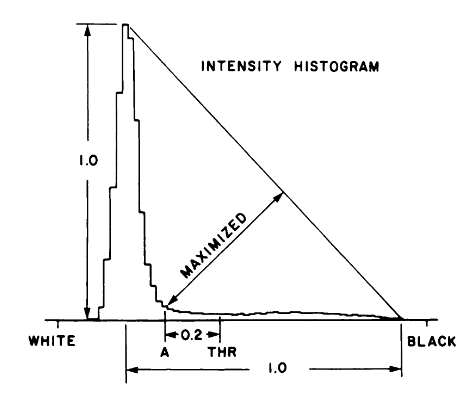
\includegraphics[scale=0.5]{figs/TriangleThresholdRef.PNG}
    \caption[Depiction of normalized histogram with annotated measurements for threshold selection]{Depiction of normalized histogram with annotated measurements for threshold selection\cite[p.742]{triangleThresh}}
    \label{fig:triangleThresh}
\end{figure}
\par This method functions well when the threshold being sought is situated close to the peak within the histogram. When this peak represents noise then the method is more effective when the angle from the peak value to the desired threshold value is steeper. If there are multiple modes in the histogram due to different noise sources or imaging properties then it can be more challenging to select an effective threshold value. This is due to the likelihood of the maximal perpendicular lengths being jointly dependent on the observed bin's closeness to the peak bin and the bin count value where the likelihood increases as the observed bin tends to the peak bin and the bin count value is lower. Figure \ref{fig:triangles} shows a series of hypothetical triangles to illustrate the impact of histogram shape on the threshold value calculations. In Fig. \ref{subfig:triangleA} the perpendicular lengths range from $L1$ to $L3$ with the chosen thresholds following the same order (to say that if $L1$ was ignored then $L2$ would be the next best threshold) where these distances are a limited subset for illustration, all bin count values will have a corresponding length. In Fig. \ref{subfig:triangleB} and \ref{subfig:triangleC} the effect of the histogram shape can be seen where the former depicts either a bimodal or dominant background bimodal histogram while the latter depicts a multimodal histogram. The bimodal histogram still presents the lowest illustrated bin value corresponding to $L1$ as the best threshold since the separation between the two modes allows a large length to that bin. The multimodal histogram shows that the multiple modes, or crests, increase the difficulty in selecting the correct threshold as there is no clear separation and both $L1$ and $L2$ are similar in value (Fig. \ref{subfig:triangleC}). Image contrast can stretch the histogram providing greater resolution to separate these modes and false modes induced by noise in the image (making it appear multimodal) can impair the effectiveness of this threshold. Based on this Triangle thresholding is effective when there are bimodal or dominant background histograms but is sensitive to noise and inappropriate adjustments to the histogram shape. \textcolor{red}{The main references are towards the beginning of this subsection which also informs later explanations but I did not explicitly reference them as part of this is from my inference of the method. Do you think I should cite those same sources again at this later point for credibility?}

\begin{figure}
\centering
\begin{subfigure}[t]{0.3\textwidth}
    \centering
    \resizebox{!}{4.4cm}{
    \input{figs/TriangleFigA.tikz}
    }
    \caption{Depiction of the perpendicular lengths from the triangle hypotenuse to the $x$-axis}
    \label{subfig:triangleA}
\end{subfigure}
\hfill
\begin{subfigure}[t]{0.3\textwidth}
    \centering
    \resizebox{!}{4.4cm}{
    \input{figs/TriangleFigB.tikz}
    }
    \caption{A slope shape that is steep but shows the impact of a crest at higher bin values due to $L2$ and $L3$ being similar.}
    \label{subfig:triangleB}
\end{subfigure}
\hfill
\begin{subfigure}[t]{0.3\textwidth}
    \centering
    \resizebox{!}{4.4cm}{
    \input{figs/TriangleFigC.tikz}
    }
    \caption{A different slope shape with a secondary, smaller peak branching off of the decline from the first peak.}
    \label{subfig:triangleC}
\end{subfigure}
\caption[A depiction of the typical trend in perpendicular distances $L$ relative to the slope shape]{A depiction of the typical trend in perpendicular distances $L$ relative to the slope shape. \subref{subfig:triangleA}) The histogram with no slope visible showing the lower $x$-axis (bin) values result in larger perpendicular distances. The impact of the slope shape is evident in (\subref{subfig:triangleB}) and (\subref{subfig:triangleC}) where the steepness in (\subref{subfig:triangleB}) results in $L1$ being the largest distance while $L2$ and $L3$ are similar despite $L2$ having a lower bin value. \subref{subfig:triangleC}) Shows the impact of a secondary peak branching off of the slope can lead to two similar lengths at different bin values. The bin ($x$-axis) value resulting in the largest perpendicular distance is used as the threshold}
\label{fig:triangles}
\end{figure}

\subsection{Richardson-Lucy deconvolution}\label{subsec:richardson_lucy}
The Richardson-Lucy (RL) deconvolution algorithm is based on the combination of two independently developed algorithms by W. Richardson~\cite{Richardson} and L. Lucy~\cite{LucyL}. For this exploration, the logic behind the algorithm will be described from W. Richardson's paper~\cite{Richardson} as it was more general focusing on image restoration as opposed to L. Lucy's~\cite{LucyL} application in the astronomical sciences field. RL deconvolution is an iterative algorithm that utilizes successive iterations to approximate a solution to minimize image diffraction. The development of this algorithm relied on a set of assumptions such as the distorted image can be represented as $H=W*S$ where $H$ is the distorted image, $W$ is the original image before distortion and $S$ is the PSF representing the diffraction which distorts the image. The second assumption is that $W$, $S$ and $H$ are probability-frequency functions such that if $i$ were some observed outcome of an event and there are $I$ total possible outcomes where $i \in I$ then there will be multiple observations $N$ where each outcome will be observed $n$ times where $n \in N$. As this is a probability-frequency function the probability of each event outcome comes to be measured from the frequency of said outcome relative to the total number of observed outcomes e.g. $P(W=W_i) = \frac{W_i}{\sum^I W_i} = \frac{n_i}{N}$. From this $W = \sum_I W_i$ where each of these function probabilities can be reduced to the observance count per outcome divided by the total number of observations across all possible outcomes. Using a single dimension $i$ is merely for descriptive simplicity and this can be expanded to multiple dimensions such that $W = \sum_{i,j} W_{i,j}$ and both $i$ and $j$ can be employed as the axis of an array or the coordinates of the pixels in an image where the outcome would be the intensity value of the pixel.\par The crux of the method relies on two equations. The first equation is the application of Baye's theorem regarding the conditional probability of an event $W_i$ given an event $H_k$ where $k$ is some observed outcome independent of $i$. The resulting formula (Eq. \ref{eq:RichBayes})~\cite[Eq. 1]{Richardson}:
\begin{equation}\label{eq:RichBayes}
    P(W_i|H_k)=\frac{P(H_k|W_i)P(W_i)}{\sum_j P(H_k|W_j)P(W_j)};\text{ }i=\{1,I\}\text{ }j=\{1,J\},\text{ }k=\{1, K\}
\end{equation}
where $H_k$ is described to be some arbitrary cell $k$ of $H$. This relationship is important as the probability of determining the correct value of $W_i$ depends on the value of $H_k$ as $H$ is the distorted image from $W$ must be restored while $W$ is not known. Since $S$ is the function of the distortion applied to each event $i$ of $W$ resulting in $H$ for some $k$ value(s) thus $P(H_k|W_i)=P(S_{i,k})=\frac{S_{i,k}}{S}$. A second consideration is that since $W_i$ is not known then the best solution is to use an estimated $W_i$ where a better estimate will result in a more accurate $W_i$. To approach this accurate $W_i$ the process is performed iteratively where each $W_i$ determined in a prior iteration is used as an estimate for the current $W_i$ estimation where $r$ is used to refer to the current iteration~\cite[Eq. 4]{Richardson}. Using both of these considerations an equation(Eq. \ref{eq:iterativeBaye})~\cite[Eq. 5]{Richardson} is determined:
\begin{equation}\label{eq:iterativeBaye}
    W_{i,r+1} = W_{i,r}\sum_k \frac{S_{i,k}H_k}{\sum_j S_{j,k}W_{j,r}}
\end{equation}
One final consideration is made due to the finite size of arrays in computers and equation \ref{eq:iterativeBaye} is changed in terms of the event summation bounds. The rewritten equation\cite[Eq. 6]{Richardson} is:
\begin{equation}\label{eq:RichardsonFinite}
    W_{i,r+1} = W_{i,r}\sum_{k=i}^c \frac{S_{k-i+1}H_k}{\sum_{j=a}^b S_{k-j+1}W_{j,r}}
\end{equation}
Where in equation \ref{eq:RichardsonFinite}, $a=(1, k-J+1)_{max}$, $b=(k,I)_{min}$, and $c=i+J-1$.For equation \ref{eq:RichardsonFinite}, W. Richardson describes that the summation over $k$ and the summation with the bounds $a$ and $b$ in the denominator appear to be a corrective measure to adjust the estimated $W_i$ over successive iterations where the denominator can compensate for escalating in value and encouraging the estimated $W_i$ to converge to some value. This compensation in one estimated element $W_{i,r}$ may be further from the final converged $W_{i,R}$ value at some iteration to improve the convergence of some other element $W_{m,r}$ where $m\in I$. The event element $i$ is one dimensional but the element variables can be expanded to account for multiple dimension arrays. A shortcoming of this algorithm is the potential for noise amplification of successive iterations although an algorithm developed from Richardson-Lucy is \textit{Richardson-Lucy with total-variation regularization} which implements a regularization term to compensate for the noise amplification~\cite[p.33]{DeconLab2}. 
\textcolor{red}{In this subsection I initially prefaced that the explanation will be based on W. Richardson's paper and I cite the individual equations I mention from his paper. Despite this do you think I need to cite him more frequently across this section?}

\section{Other techniques implemented within this research}

\subsection{Kneedle algorithm} \label{sec:kneedle}
\textit{Kneedle} is an approach to determine `knees' in a distribution~\cite{kneedle_paper}. Traditionally the knee, or elbow, of a distribution is described as some approximate point by which there is a change in the trend of the distribution. This is similar to the concept of the inflection point of the distribution but there is no standardised definition of a `knee' rather it is the visual estimation of the point performed heuristically by a human viewing the visualisation of the data. Due to this, it can be loosely defined as the point most significant to the change in the trend of the data. A visualised distribution with an estimated region in which a `knee' would be selected is shown in Figure \ref{fig:knees}.\par
\begin{figure}
    \centering
    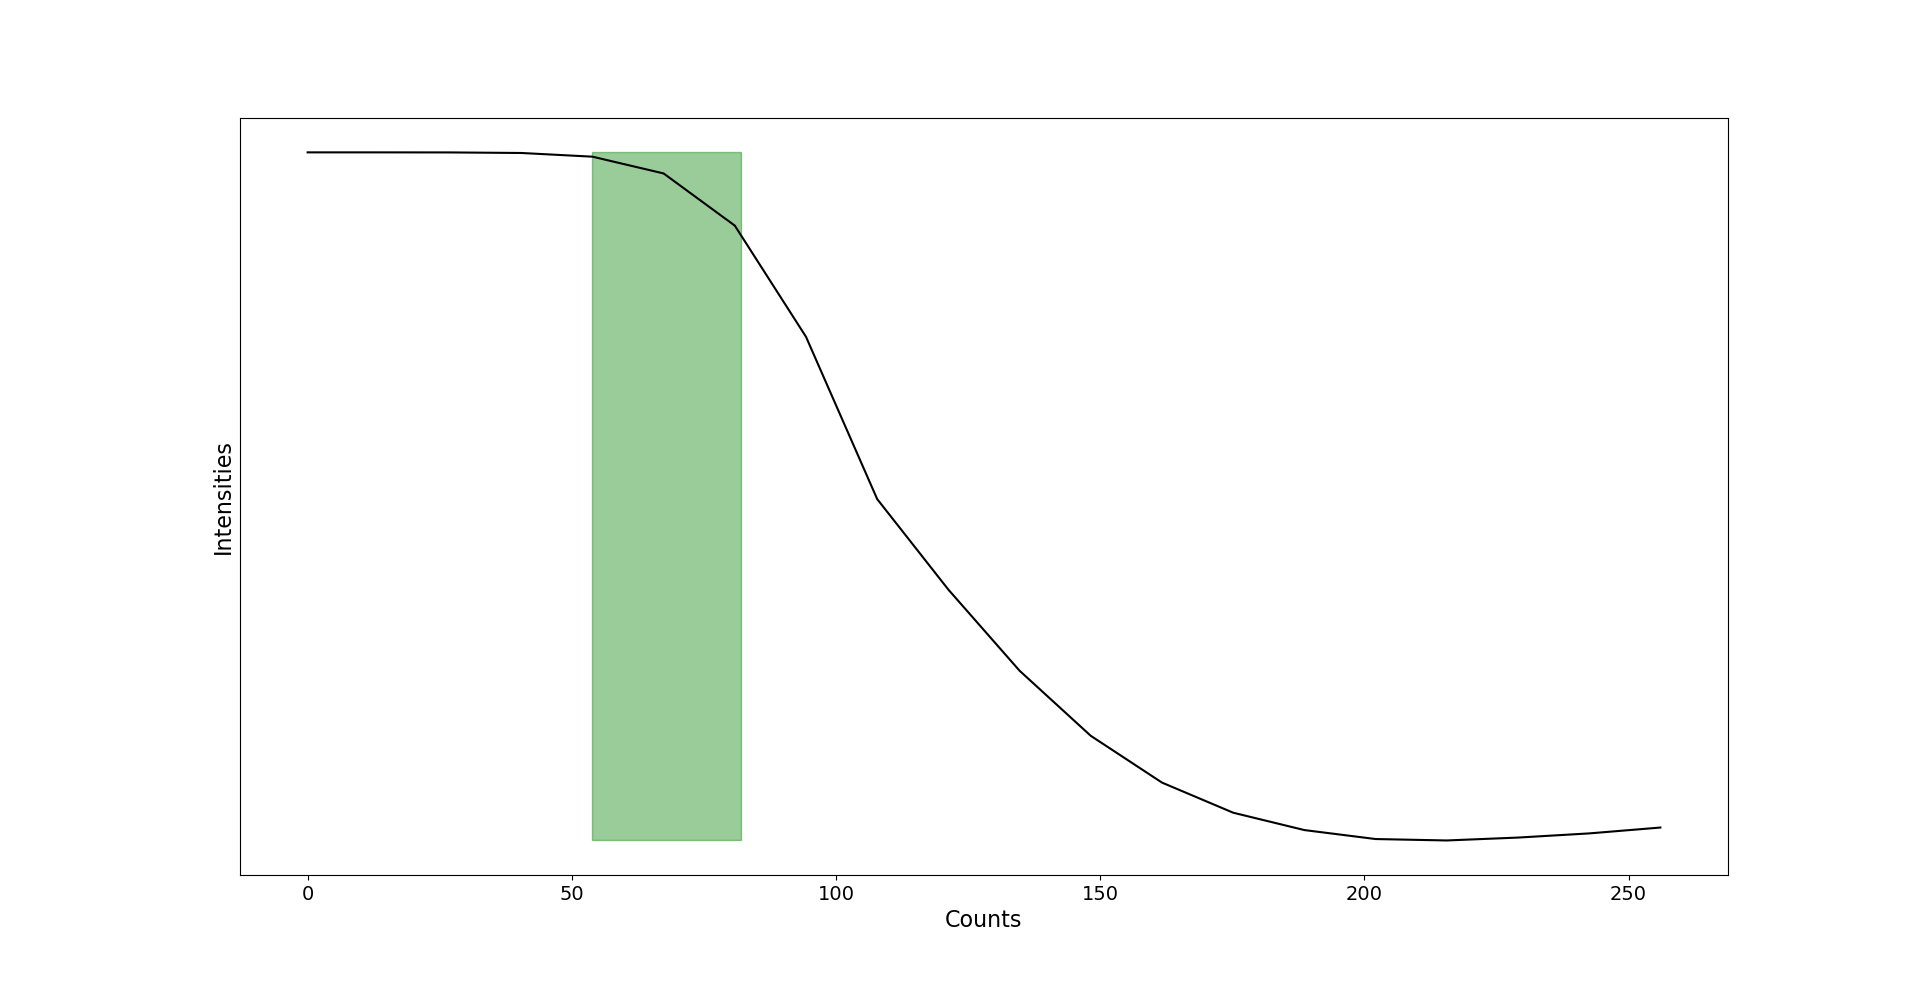
\includegraphics[width=0.7\textwidth]{figs/ch2figs/knees.png}
    \caption[Approximate knees in a graph by heuristic evaluation]{Approximate knees in a graph by heuristic evaluation. The highlighted region designates the likely region within which a knee point would be chosen. A range is displayed as the exact point is dependent on heuristic bias.}
    \label{fig:knees}
\end{figure}
One method of interest that attempts to address this is \textit{Finding a ``Kneedle'' in a Haystack:Detecting Knee Points in System Behavior}~\cite{kneedle_paper} which both presents a mathematical definition of a `knee' and the method by which this `knee' is determined. \paragraph{Knee Definition} Firstly, it was stated prior that the knee of a distribution is visually similar to that of the inflection point yet this point does not capture the point at which trends change but rather a change in the sign of the curvature of the distribution. The chosen definition is based on the curvature of a continuous definition where the point at which maximum curvature is expressed is the closest to what would be the knee point~\cite[p.2]{kneedle_paper}. The equation describing curvature ($K_f(x)$) is shown in Equation \ref{eq:curvature} where $f(x)$ is the distribution for which the curvature is being described.\par
\begin{equation}\label{eq:curvature}
    K_f(x) = \frac{f''(x)}{(1 + f'(x)^2)^{1.5}}
\end{equation}
This curvature equation performs well with continuous functions yet is challenged by discrete distributions. The causes behind these challenges are related to the incompatibility encountered when fitting a continuous function to a finite distribution as a minimum of 3 data points are required to calculate the curvature (centred on the second data point) thus the curvature for the first and final point in the discrete set cannot be determined. Another major challenge is that determination of the maximum curvature within the distribution requires this calculation to be performed across the whole discrete set and it is possible for the point of maximum curvature to exist outside the range of the finite set.\paragraph{Knee method} It is explicitly stated that \textit{``Kneedle''}, the method by which the knees are determined, is predicated on the assumption that the knee is the point expressing the maximum curvature but there can be multiple knee points within a distribution or set. For multiple points to be approximated it is the local maxima of the curvature across the set that describes a knee point. These local maxima of the curvature are determined by \textit{``that are local maxima if the curve is rotated $\theta$ degrees clockwise about ($x_{min},y_{min}$) through the line formed by the points ($x_{min},y_{min}$) and ($x_{max},y_{max}$)''}~\cite[p.3]{kneedle_paper}. Thus far the designed method presumes that the knee point is for an increasing curve that is of negative concavity but this can be performed for curves with a positive concavity (an ``elbow'' as opposed to a knee) by inverting the distribution with examples for each shown in Figure \ref{fig:knee_elbow_example}.
\begin{figure}
    \centering
    \subcaptionbox{Knee example}{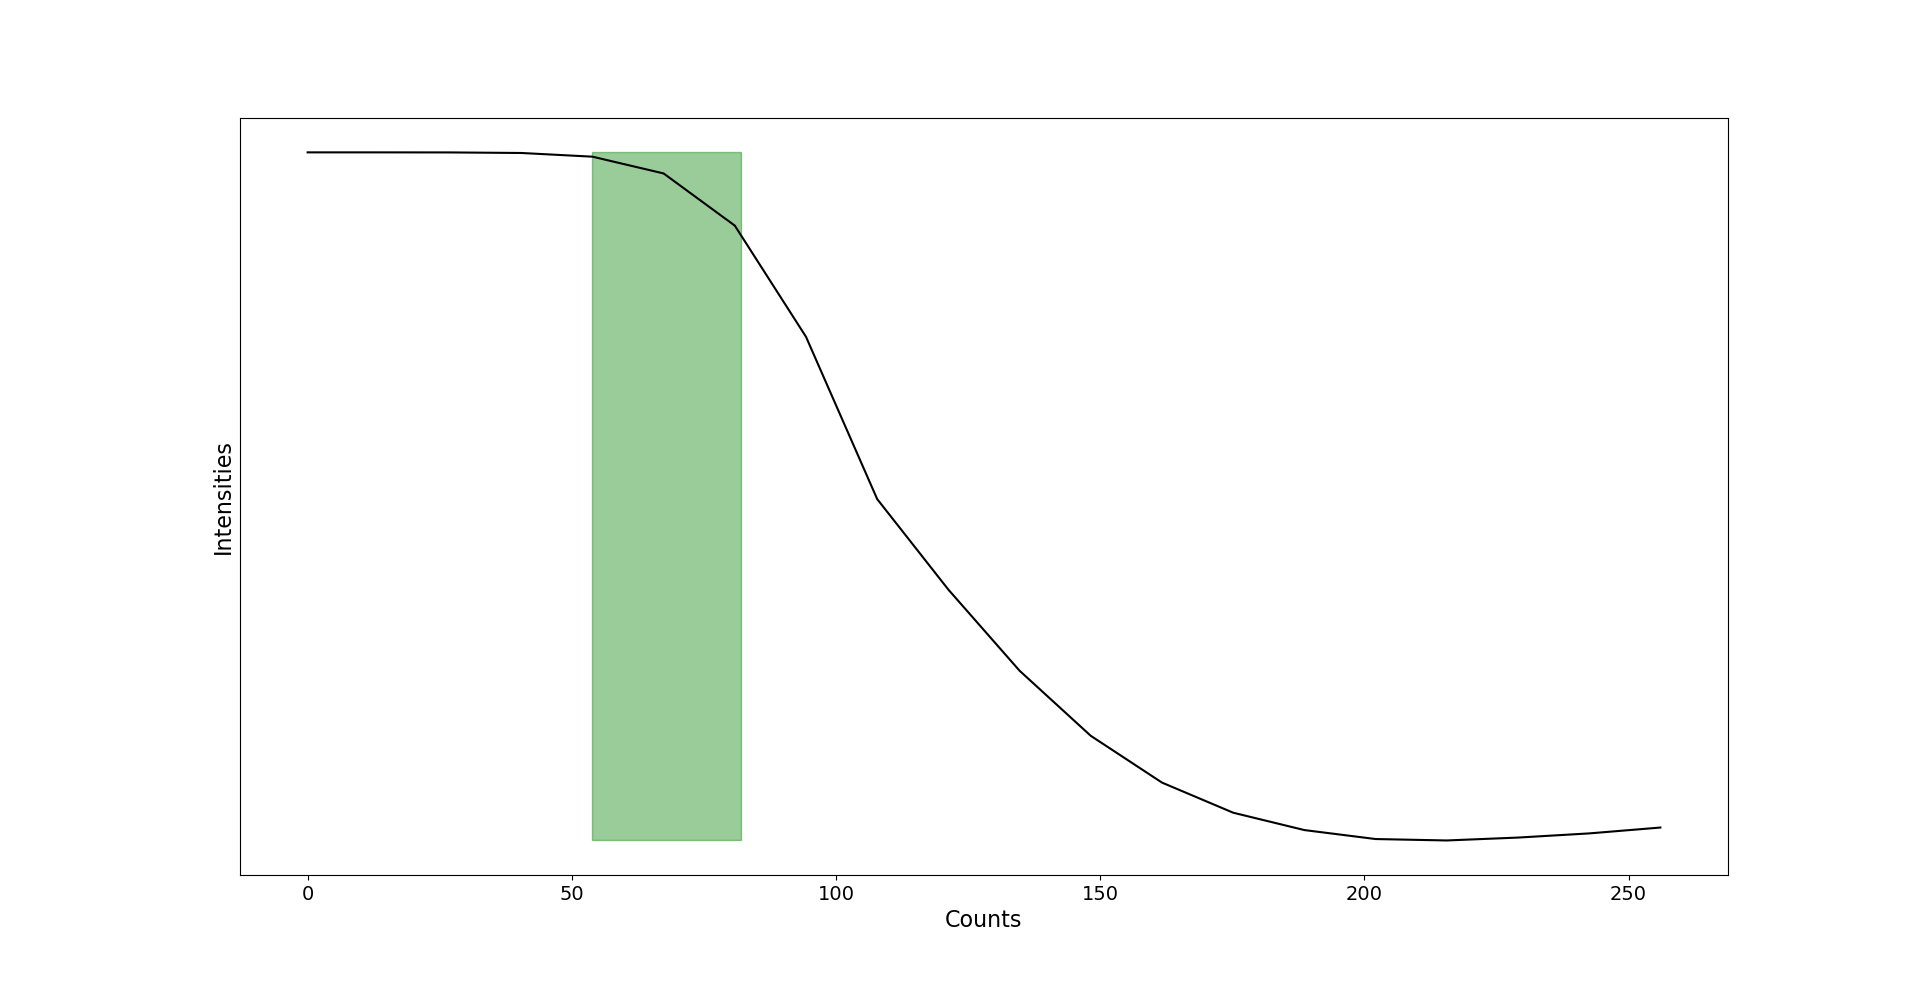
\includegraphics[width=0.49\textwidth]{figs/ch2figs/knees.png}}
    \subcaptionbox{Elbow example}{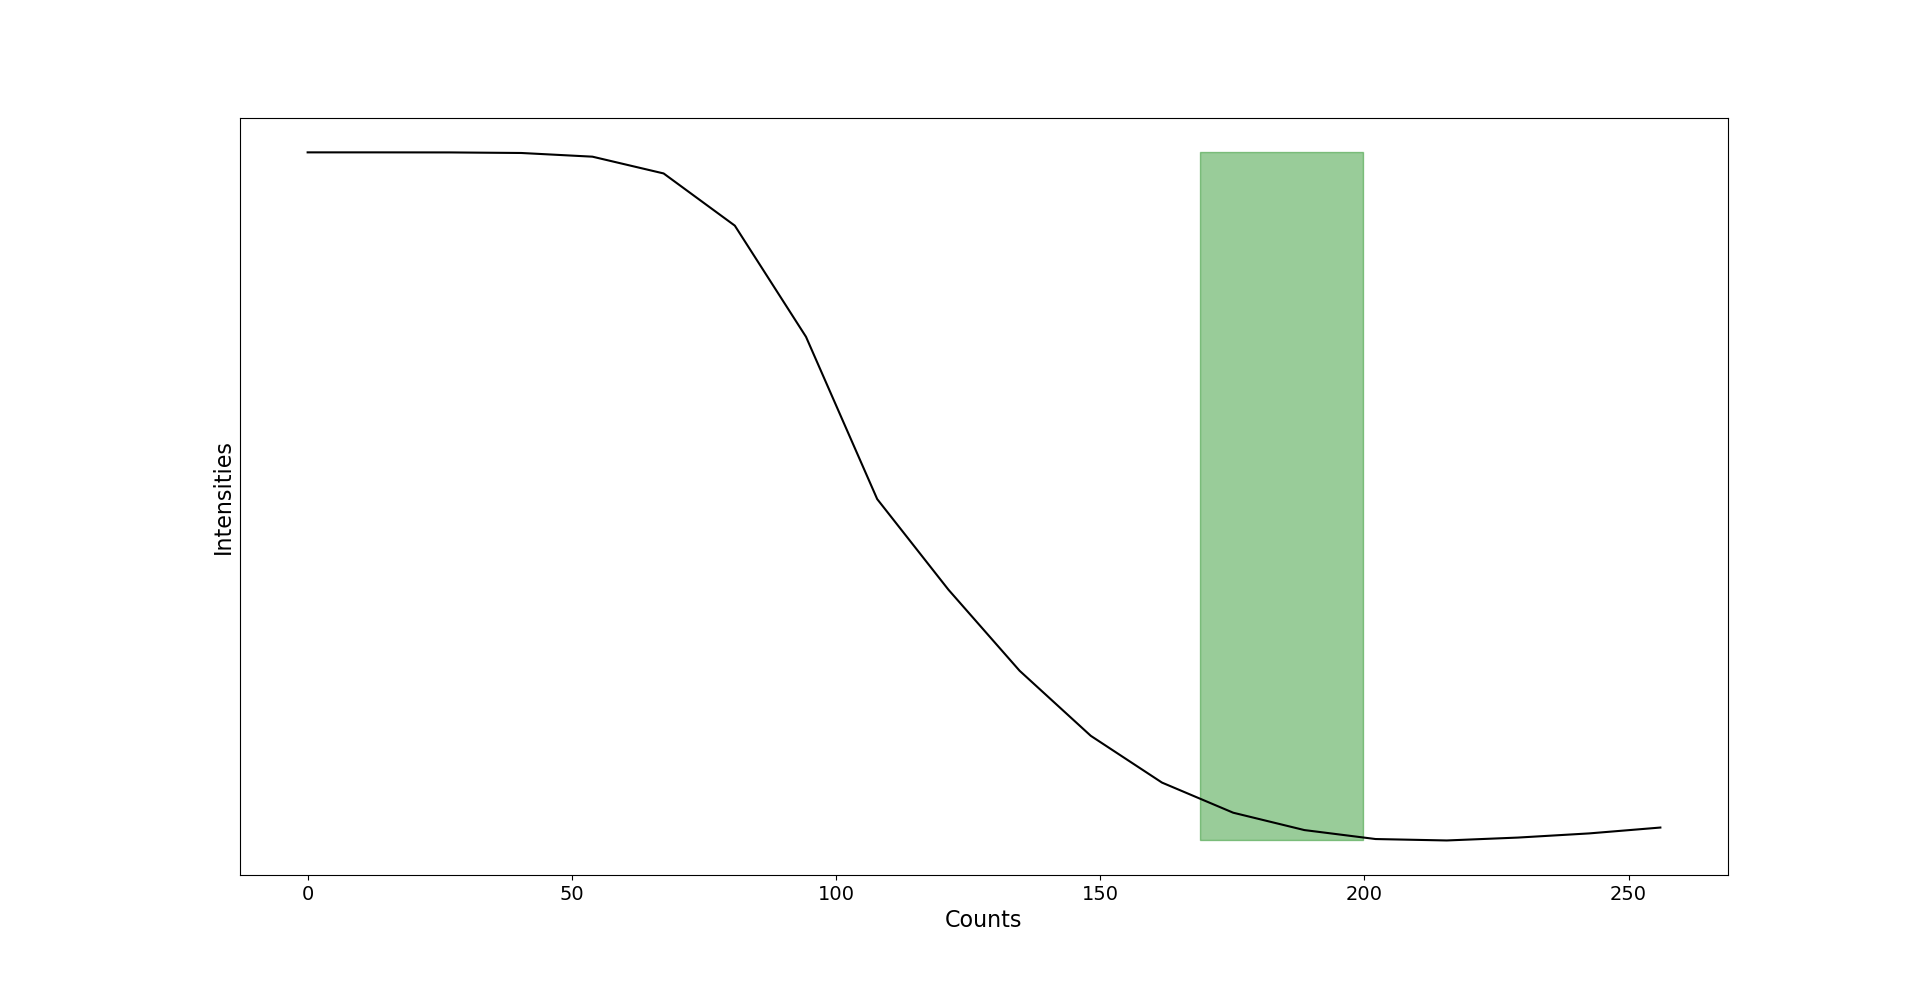
\includegraphics[width=0.49\textwidth]{figs/ch2figs/elbows.png}}
    \caption{Knee and elbow approximation regions are shown for some given distribution}
    \label{fig:knee_elbow_example}
\end{figure}
The method through which the Kneedle algorithm determines the knee points can be separated into six steps given some data set $D$ which is a finite discrete set of paired values $(x_i,y_i)$: 
\begin{enumerate}
    \item Smooth the discrete data set ($D$) to reduce the noise in the data. The retention of the shape of the set must be maximised.
    \item Normalize the finite data set points as the algorithm behaviour is independent of the point magnitudes. Both $x$ and $y$ values are normalized to a unit square while preserving their shape, as shown (Equation \ref{eq:smoothed_knee}):
    \begin{equation}\label{eq:smoothed_knee}
        \begin{split}
            D_{sn} &= \{(x_{sn},y_{sn})\},\text{ where}\\
            x_{sn_i} &= (x_{s_i}-min\{x_s\})/(max\{x_s\}-min\{x_s\})\\
            y_{sn_i} &= (y_{s_i}-min\{y_s\})/(max\{y_s\}-min\{y_s\})
        \end{split}
    \end{equation}
    \item A difference set ($D_d$) represents the differences between the $x-$ and $y-$value pairs which are mapped as ($x_{sn}, y_{sn}-x_{sn}$). This constructs a difference curve where the increases in the $y-$values are relative to the magnitude of the paired $x-$values. The insight provided by this difference curve is the behaviour it describes. When the curve transitions from horizontal to decreasing at a point indicates that said point is a potential knee.
    \item As mentioned prior, it is where the difference curve transitions from flattening to decreasing denoting the presence of a knee. Under the assumption that the points of the set are not decreasing, it is the local maxima of the difference curve that embody positions around which the rate of increase decreases noticeably. Each of these local maxima of the difference set is a candidate knee point.
    \item Each candidate knee occupies a local maxima where a certain deceleration in the smoothed data increase is perceived but the quantity of deceleration over a number of points defines what is declared as knees. At each candidate knee of the difference curve, a threshold value is calculated with a tunable sensitivity parameter ($S$). This threshold ($T_{lmx_i}$) is calculated by calculating the mean of the forward difference, with a spacing of 1, $(x_{sn_{i+1}}-x_{sn_i})$ which is multiplied by the sensitivity value ($S$) which is finally subtracted from the candidate knee value ($y_{lmx_i}$) for some candidate knee ($i$) shown in Equation \ref{eq:knee_threshold}.
    \begin{equation}\label{eq:knee_threshold}
        T_{lmx_i} = y_{lmx_i}-S\cdot \frac{\sum_{i=1}^{n-1}(x_{sn_{i+1}}-x_{sn_i})}{n-1}
    \end{equation}
    \item Each calculated threshold value is unique to each candidate knee (difference curve local maxima) and it is the decrease in the difference curve, after a candidate knee, relative to this threshold that determines whether it is a valid knee. The criteria are that the difference curve values, after a candidate knee, must decrease below the associated knee threshold ($y < T_{lmx_i}$) value prior to either increasing from a local minimum or encountering another candidate knee. If a local minimum of the difference curve is encountered, after which the curve increases, then the next candidate knee is evaluated. The smaller the sensitivity parameter ($S$) the closer the threshold to the candidate knee value (local maxima) and the easier it is to pass the criteria.
\end{enumerate}

\section{Prominent literature used in this research}
Throughout this chapter, various pieces of literature have been used in developing the system itself (detailed in Chapter \ref{ch:methodology}) or to develop an understanding of the biology and image processing that informed future decisions indirectly. For this breakdown, the literature will be separated by those that provided a foundational understanding of the fields involved with this research, those involved with the pre-processing of the image data prior to the thresholding system, and last will be the literature that was involved in the development of the automated thresholding system itself.
\subsection*{Foundational understanding}
\paragraph{Biology} The foundation of this came from a high-level understanding of the biological phenomena that describe the organelles of interest and the mitophagy process which is the process that will be analyzed after complete pre-processing. The largest contributor to understanding mitophagy and the related organelles was \textit{Human Physiology: From Cells to Systems}~\cite{cell_phys_book} which covered information regarding autophagy, the mitochondria and, to a lesser degree, mitophagy. More detailed information relating to autophagosomes, lysosomes and the relationship between the two is detailed in \textit{The discovery of lysosomes and autophagy}~\cite{lyso_auto_relation}. Detailed insight on mitophagy and its relationship with the fission and fusion of mitochondria is covered in \textit{Mitochondrial fission, fusion, and stress}~\cite{MitoFus-2012} and \textit{Mechanisms of mitophagy}~\cite{MitoMechan}. \paragraph{Microscopy} The fundamentals provided by microscopy are to recognise the causes of reduced image quality or errant phenomena observed that originate from the imaging process. A particular impact on this understanding of confocal microscopy is \textit{Fluorescence microscopy}~\cite{Sanderson-2014} but it is the constraints listed as bleed-through, photobleaching and diffraction that are the most valuable as these understanding of these constraints can inform undesired behaviours or details seen in the image during the analysis that might not relate to the actual specimen. Bleed-through was detailed by \textit{Fluorescence microscopy}~\cite{Sanderson-2014} and \textit{A guided tour into subcellular colocalization analysis in light
microscopy}~\cite{Bolte-2006}; photobleaching was informed by \textit{Photobleaching kinetics of fluorescein in
quantitative fluorescence microscopy}~\cite{photobleach_excite} and \textit{Loss of image quality in photobleaching
during microscopic imaging of fluorescent probes bound to chromatin}~\cite{photobleachingPaper}; and diffraction was informed by \textit{Diffraction-unlimited optical microscopy}~\cite{Diffraction_Patterson} and \textit{ Diffraction-unlimited optical microscopy}~\cite{Diffraction_Dedecker}.

\subsection*{Pre-processing understanding}
Since this research is exploring and developing an automated high-throughput thresholding system it is important to understand other pre-processing techniques that are applied to the image prior to the application of the system. Likewise understanding the influence of these techniques regarding the manner in which they improve image quality (noise removal, signal enhancement, etc.) is crucial as each of these methods can impart an undue effect on the image as a byproduct of their process and mitigate these byproducts using subsequent pre-processing techniques, including the automated thresholding. An overview of deconvolution, the generation of the PSF, and a high-level mathematical representation of the diffraction effect and its removal via deconvolution is described by \textit{3D PSF models for fluorescence microscopy in ImageJ}~\cite{psfgen} for the generation of synthetic PSFs, and by both \textit{Blind deconvolution of gaussian blurred images containing additive
white gaussian noise}~\cite{6505824} and \textit{Deconvolutionlab2: An open-source software for deconvolution microscopy}~\cite{DeconLab2} in terms of the mathematical representation. For denoising, a statistical understanding of noise (not artefacts or bleed-through) is provided by \textit{Analyzing fluorescence microscopy images with ImageJ}~\cite{bioimage_book} while the behaviour of standard denoising filters is informed by median and Gaussian filters but also by the Sigma filter~\cite{sigma_filter}. For image enhancement, the primary insight developed was through analysis of two such methods for background subtraction and contrast enhancement described by \textit{Biomedical image processing}~\cite{rolling_ball} and \textit{Contrast Limited Adaptive Histogram Equalization}~\cite{clahe} respectively. The last group of methods were those relating to thresholding which is separated into global and local methods that segment the image into foreground and background thus binarizing it. Thresholding as a whole was described by \textit{Chapter 9 - image segmentation}~\cite{segmentation_book} in the context of image segmentation while further detail regarding global and local methods was informed by \cite{Otsu1979ATS} and \textit{Analyzing fluorescence microscopy images with ImageJ}~\cite{bioimage_book}. These pre-processing methods were all to be applied sequentially within a pipeline and a paper which stimulated the exploration into why these methods are applied sequentially was provided by \textit{A pipeline for multidimensional confocal analysis of
mitochondrial morphology, function, and dynamics in pancreatic $\beta$-cells}~\cite{PipelineDecon-Chaudhry}.

\subsection*{Literature that directly impacted system design}
The research that directly featured in the automated thresholding system being developed or that was compared against for evaluation consists of a number of thresholding techniques and other algorithms. These thresholding techniques are the Otsu threshold~\cite{Otsu1979ATS}) and Triangle threshold~\cite{triangleThresh} as they are both automated threshold methods reliant on image histogram being bimodal or close to. Hysteresis thresholding, proposed by \cite{Hysteresis}, is important as it forms the backbone of the system design while the Kneedle algorithm~\cite{kneedle_paper} is an unconventional approach for low threshold approximation detailed in Chapter \ref{ch:methodology}.  

\section{Chapter conclusions}
%This chapter conveys a body of information providing context behind choices made throughout this project. Some of these choices were determined externally by the mitophagy research application case of this project while others were design decisions made during the development of the high-throughput thresholding system. References to the information covered in this section will be made in Chapter 3 where other research related to cellular microscopy thresholding, subcellular microscopy thresholding and automatic thresholding are explored. Chapter 4 describes two main components with the first relating to the image acquisition and processing prior to the thresholding system application and the second being the design of the thresholding system.  

This chapter conveyed theory and concepts relating to the techniques that will be implemented or are to be explored throughout this work. This theory extended from providing context around the approaches dictated by the mitophagy research use case to those being explored for implementation in the high-throughput thresholding system design. The mitophagy research use case determines the objects to be imaged (Section \ref{sec:mito_detail}), the microscopy technique to be used (Section \ref{sec:fluorMicr}), and the analysis approach (colocalisation) that the images must be of suitable quality for (Section \ref{sec:coloc}).\par The thresholding system being designed is not expected to function in isolation with a number of adjacent approaches applied before or after the system to maximise the restored image quality. For this reason, the context was provided regarding factors of image quality degradation (Section \ref{sec:Noises}), a high-level overview of the sequential application of approaches to improve the image quality (Section \ref{subsec:pipe}), and a high-level overview of these approaches grouping them by the aspect of image quality that is addressed (Section \ref{sec:overview_preproc_methods}). There is also a deeper discussion on the theory surrounding specific approaches of interest to this work (Section \ref{sec:further_methods}).\par This chapter serves to consolidate and organise all of the theoretical backgrounds of phenomena, techniques and approaches that inform design choices and observed behaviours of the high-throughput thresholding system. The proceeding chapters (Chapter \ref{ch:methodology} and Chapter \ref{ch:results}) both reference this chapter in terms of both the specimens and imaging techniques used for image acquisition, and the techniques implemented in the system design to develop a high-throughput thresholding system. 
 